%\documentclass[table]{article}
%\usepackage{beamerarticle}
\documentclass[10pt,xcolor=table,ignorenonframetext,handout,aspectratio=169]{beamer}
%\documentclass[10pt,xcolor=table,ignorenonframetext]{beamer}
\mode<presentation>
{
  \usetheme{default}
  \useoutertheme{split}
% \usefonttheme{serif}
}

\usenavigationsymbolstemplate{}
\usepackage{amssymb}
\usepackage{amsmath}
\usepackage{setspace}
\usepackage{graphicx}
\usepackage{multirow}
\usepackage[english]{babel}
\usepackage[latin1]{inputenc}
\usepackage{bm}
\usepackage{graphicx}
\usepackage{multirow}
\usepackage{tikz}
\usepackage[english]{babel}
\usepackage[latin1]{inputenc}
%\usepackage{ulem}
\usepackage{pifont}
\usepackage{changepage}
%\usepackage{colortbl}
%\usepackage[table]{xcolor}
%\usepackage{xcolor}

\setbeamersize{text margin left=1cm,text margin right=5cm}

\setbeamertemplate{itemize item}[circle]
\setbeamertemplate{frametitle}[default][center]

\newlength{\wideitemsep}
\setlength{\wideitemsep}{\itemsep}
\addtolength{\wideitemsep}{4pt}
\let\olditem\item
\renewcommand{\item}{\setlength{\itemsep}{\wideitemsep}\olditem}

\newcommand{\HRule}{\rule{0.5\textwidth}{0.05mm}}

\usetikzlibrary{arrows,positioning,shapes}
\usetikzlibrary{decorations.pathreplacing}

\definecolor{blueish}{RGB}{97,156,255}
\definecolor{greenish}{RGB}{0,186,56}
\definecolor{reddish}{RGB}{248,118,109}

\definecolor{oiverm}{RGB}{213,94,0}
\definecolor{oiblue}{RGB}{0,114,178}
\definecolor{oigreen}{RGB}{0,158,115}
\definecolor{oipurple}{RGB}{204,121,167}
\definecolor{oiorange}{RGB}{230,159,0}
\definecolor{oisky}{RGB}{86,180,233}
\definecolor{oiyellow}{RGB}{240,228,66}
\definecolor{williams}{RGB}{81,38,152}

\definecolor{hue1}{RGB}{255,255,204}
\definecolor{hue2}{RGB}{161,218,180}
\definecolor{hue3}{RGB}{65,182,196}
\definecolor{hue4}{RGB}{44,127,184}
\definecolor{hue5}{RGB}{37,52,148}

\definecolor{dvg1}{RGB}{213,62,79}
\definecolor{dvg2}{RGB}{244,109,67}
\definecolor{dvg3}{RGB}{253,174,97}
\definecolor{dvg4}{RGB}{254,224,139}
\definecolor{dvg5}{RGB}{230,245,152}
\definecolor{dvg6}{RGB}{171,221,164}
\definecolor{dvg7}{RGB}{102,194,165}
\definecolor{dvg8}{RGB}{50,136,189}

\setbeamercolor{structure}{fg=williams,bg=williams!12}

\title{Difference-in-Differences, Slide \insertframenumber}
\subtitle{}

\author{Economics 379 (Professor Jakiela)}
\date{}



\begin{document}
	
	
	
%%%%%%%%%%%%%%%%%%%%%%%%%%%%%%%%%%%%%%%%%%%%%%%%%%%%%%%%%%%%%%%%%%%%%%%%%%
	% COURSE Title slide
%%%%%%%%%%%%%%%%%%%%%%%%%%%%%%%%%%%%%%%%%%%%%%%%%%%%%%%%%%%%%%%%%%%%%%%%%%
	
\begin{frame}<beamer:0>[plain]
	
	\begin{center}
		\begin{tikzpicture}
		
		\node [opacity=1] (bg)  {\includegraphics[keepaspectratio,height=0.9\paperheight]{photos/Kenya-cistern-Flore-de-Preneuf-2011-LARGE.jpg}};
		
		\node [anchor=east,align=right] at (6,-2.25) {\Large{\textcolor{white}{Williams College ECON 379:}}};		
		\node [anchor=east,align=right] at (6,-3) {\Large{\textcolor{white}{Program Evaluation for International Development}}};

		\node [anchor=east] at (6,-3.8) {\textcolor{yellow}{\tiny{photo:  Flore de Preneuf / World Bank}}};
		
		\end{tikzpicture}
	\end{center}
\end{frame}


%%%%%%%%%%%%%%%%%%%%%%%%%%%%%%%%%%%%%%%%%%%%%%%%%%%%%%%%%%%%%%%%%%%%%%%%%%
% LECTURE Title slide
%%%%%%%%%%%%%%%%%%%%%%%%%%%%%%%%%%%%%%%%%%%%%%%%%%%%%%%%%%%%%%%%%%%%%%%%%%

\begin{frame}[plain]

\begin{adjustwidth}{0cm}{-4cm}

\begin{center}
	\begin{tikzpicture}
	
	\node [opacity=0.25] (bg)  {\includegraphics[keepaspectratio,height=0.9\paperheight]{photos/Senegal-WAAPP-seeds-Daniella-Van-Leggelo-Padilla-LARGE.jpg}};
	
	\node at (0,2.5) {\large{\textcolor{williams}{Williams College ECON 379:}}};		
	\node at (0,1.5) {\large{\textcolor{williams}{Program Evaluation for International Development}}};
	
	\node at (0,-0.5) {\large{\textcolor{williams}{\textbf{Module 4: Difference-in-Differences}}}};
	
	\node at (0,-2) {\large{\textcolor{williams}{Professor:  Pamela Jakiela}}};
	
	\node [anchor=east] at (6,-3.8) {\textcolor{yellow}{\tiny{photo:  Daniella Van Leggelo-Padilla / World Bank}}};
	
	\end{tikzpicture}
\end{center}
\end{adjustwidth}
\end{frame}



%%%%%%%%%%%%%%%%%%%%%%%%%%%%%%%%%%%%%%%%%%%%%%%%%%%%%%%%%%%%%%%%%%%%%%%%%%%

\begin{frame}[plain]

\begin{adjustwidth}{0cm}{-4cm}

\begin{center}
	
\Large{Intuition}
	
\end{center}

\end{adjustwidth}
\end{frame}


%%%%%%%%%%%%%%%%%%%%%%%%%%%%%%%%%%%%%%%%%%%%%%%%%%%%%%%%%%%%%%%%%%%%%%%
%
%\begin{frame}{Do Hospitals Make People Healthier?}
%
%\begin{center}
%	\begin{tikzpicture}
%	
%	% blank canvas
%	\only<handout>{\fill[fill=white,draw=white,ultra thin]
%	(0,0) -- (11,0) -- (11,6) -- (0,6) -- cycle;}
%	\only<beamer>{\fill[fill=white,draw=white,ultra thin]
%	(0,0) -- (14,0) -- (14,6) -- (0,6) -- cycle;}
%	\only<beamer>{\draw[draw=oiblue!60,fill=oiblue!10,opacity=0.5] (11,1) rectangle (14,5);}
%	\draw[step=1.0,gray!20,thin] (0,0) grid (11,6);
%	
%	\pgfmathsetmacro\xshift{0.5cm};
%	\pgfmathsetmacro\yshift{5.5cm};
%	\pgfmathsetmacro\mycolor{"gray"};
%	
%	\node[anchor=north west,align=left,text width = 9.5cm,xshift=\xshift,yshift=\yshift] (text1) at (0,0) {My long two pointed ladder is sticking through a tree toward heaven still and there is a barrel that I didn't fill beside it and there may be two or three apples that I did not pick upon some bow but I am done with apple picking now.  Essence of winter sleep is on the night the sent of apples I am drowsing off I cannot rub the strangeness from my sight I got from looking through a pane of glass I skimmed this morning from the drinking trough and held against a world of hoary grass. It melted and I let it fall and break but I was well upon my way to sleep before it fell and I could tell what form my dreaming was about to take.  Magnified apples appear and disappear stem end and blossom end and every fleck of russet showing clear.};
%	
%	\end{tikzpicture}
%\end{center}
%\end{frame}



%%%%%%%%%%%%%%%%%%%%%%%%%%%%%%%%%%%%%%%%%%%%%%%%%%%%%%%%%%%%%%%%%%%%%

\begin{frame}{False Counterfactuals}

\medskip
\textbf{Before vs.~After Comparisons:}

\medskip
\begin{itemize}
	
	\item
	\textbf{Compares:} same units before/after program
	
	\item
	\textbf{Drawback:} does not control for time trends
	
\end{itemize}

\medskip
\textbf{Participant vs.~Non-Participant Comparisons:}

\medskip
\begin{itemize}
	
	\item
	\textbf{Compares:} participants to those not in the program
	
	\item
	\textbf{Drawback:} potential for selection bias \\
	\emph{Are participants different in absence of treatment?}
	
\end{itemize}

\end{frame}


%%%%%%%%%%%%%%%%%%%%%%%%%%%%%%%%%%%%%%%%%%%%%%%%%%%%%%%%%%%%%%%%%%%%%

\begin{frame}{Two Wrongs Sometimes Make a Right}

\medskip

\textbf{Difference-in-differences} estimation (or ``diff-in-diff'' or ``DD'') combines the two (flawed) false counterfactual approaches

\medskip
\begin{itemize}
	
	\item Observe self-selected treatment group, comparison groups before and after treatment group participates in treatment
	
	\item May overcome problems of both when [1] selection bias is on fixed traits of units and [2] time trends common to both groups

	
\end{itemize}

\pause
\medskip
\medskip

\textbf{The diff-in-diff estimator is:}
\begin{equation*}
DD = \textcolor{black}{\bar{Y}^{treatment}_{post} - \bar{Y}^{treatment}_{pre}} - \left( \textcolor{black}{\bar{Y}^{comparison}_{post} - \bar{Y}^{comparison}_{pre}}  \right)
\end{equation*}

\end{frame}




%%%%%%%%%%%%%%%%%%%%%%%%%%%%%%%%%%%%%%%%%%%%%%%%%%%%%%%%%%%%%%%%%%%%%

\begin{frame}<handout:0>{Two Wrongs Sometimes Make a Right}

\medskip

\textbf{Difference-in-differences} estimation (or ``diff-in-diff'' or ``DD'') combines the two (flawed) false counterfactual approaches

\medskip
\begin{itemize}
	
	\item Observe self-selected treatment group, comparison groups before and after treatment group participates in treatment
	
	\item May overcome problems of both when [1] selection bias is on fixed traits of units and [2] time trends common to both groups
	
	
\end{itemize}

%\pause
\medskip
\medskip

\textbf{The diff-in-diff estimator is:}
\begin{equation*}
DD = \textcolor{red}{\bar{Y}^{treatment}_{post} - \bar{Y}^{treatment}_{pre}} - \left( \textcolor{black}{\bar{Y}^{comparison}_{post} - \bar{Y}^{comparison}_{pre}}  \right)
\end{equation*}

\end{frame}


%%%%%%%%%%%%%%%%%%%%%%%%%%%%%%%%%%%%%%%%%%%%%%%%%%%%%%%%%%%%%%%%%%%%%

\begin{frame}<handout:0>{Two Wrongs Sometimes Make a Right}

\medskip

\textbf{Difference-in-differences} estimation (or ``diff-in-diff'' or ``DD'') combines the two (flawed) false counterfactual approaches

\medskip
\begin{itemize}
	
	\item Observe self-selected treatment group, comparison groups before and after treatment group participates in treatment
	
	\item May overcome problems of both when [1] selection bias is on fixed traits of units and [2] time trends common to both groups
	
	
\end{itemize}

%\pause
\medskip
\medskip

\textbf{The diff-in-diff estimator is:}
\begin{equation*}
DD = \textcolor{black}{\bar{Y}^{treatment}_{post} - \bar{Y}^{treatment}_{pre}} - \left( \textcolor{red}{\bar{Y}^{comparison}_{post} - \bar{Y}^{comparison}_{pre}}  \right)
\end{equation*}

\end{frame}



%%%%%%%%%%%%%%%%%%%%%%%%%%%%%%%%%%%%%%%%%%%%%%%%%%%%%%%%%%%%%%%%%%%%%%%

\begin{frame}{Difference-in-Differences Estimation}

\begin{center}
	\begin{tikzpicture}
	
	% blank canvas
	\only<handout>{\fill[fill=white,draw=white,ultra thin]
	(0,0) -- (11,0) -- (11,6) -- (0,6) -- cycle;}
	\only<beamer>{\fill[fill=white,draw=white,ultra thin]
	(0,0) -- (14,0) -- (14,6) -- (0,6) -- cycle;}
	\only<beamer>{\draw[draw=oiblue!60,fill=oiblue!10,opacity=0.5] (11,1) rectangle (14,5);}
	%\draw[step=1.0,gray!20,thin] (0,0) grid (11,6);
	
	\pgfmathsetmacro\xshift{5cm};
	\pgfmathsetmacro\yshift{4cm};
	
% 2X2 grid with labels
\pgfmathsetmacro\mycolor{"black"};
\draw[\mycolor,thick,xshift=\xshift,yshift=\yshift] (-2,-1) -- (2,-1) -- (2,1) -- (-2,1) -- cycle;
\draw[\mycolor,thick,xshift=\xshift,yshift=\yshift] (-2,0) -- (2,0);
\draw[\mycolor,thick,xshift=\xshift,yshift=\yshift] (0,-1) -- (0,1);
\node[\mycolor,anchor=east,align=right,xshift=\xshift,yshift=\yshift] at (-2,0.5) {pre-program};
\node[\mycolor,anchor=east,align=right,xshift=\xshift,yshift=\yshift] at (-2,-0.5) {post-program};
\node[\mycolor,anchor=south,xshift=\xshift,yshift=\yshift] at (-1,1) {\textcolor{white}{p}treatment\textcolor{white}{p}};
\node[\mycolor,anchor=south,xshift=\xshift,yshift=\yshift] at (1,1) {\textcolor{white}{p}comparison\textcolor{white}{p}};

% cell contents
\node[\mycolor,xshift=\xshift,yshift=\yshift] at (-1,0.5) {$\bar{Y}^{treatment}_{pre}$};
\node[\mycolor,xshift=\xshift,yshift=\yshift] at (1,0.5) {$\bar{Y}^{comparison}_{pre}$};
\node[\mycolor,xshift=\xshift,yshift=\yshift] at (-1,-0.5) {$\bar{Y}^{treatment}_{post}$};
\node[\mycolor,xshift=\xshift,yshift=\yshift] at (1,-0.5) {$\bar{Y}^{comparison}_{post}$};

% text
\node[anchor=west,align=left,xshift=\xshift,yshift=\yshift] at (-4.75,-2) {Diff-in-diff estimation is just a comparison of 4 cell-level means};
%\node[anchor=west,align=left,xshift=\xshift,yshift=\yshift] at (-4.25,-2.75) {\structure{$\Rightarrow$} Only one cell is treated:  \textbf{treatment}$\times$\textbf{post-program}};
	
	\end{tikzpicture}
\end{center}
\end{frame}


%%%%%%%%%%%%%%%%%%%%%%%%%%%%%%%%%%%%%%%%%%%%%%%%%%%%%%%%%%%%%%%%%%%%%%%

\begin{frame}<handout:0>{Difference-in-Differences Estimation}

\begin{center}
	\begin{tikzpicture}
	
	% blank canvas
	\only<handout>{\fill[fill=white,draw=white,ultra thin]
		(0,0) -- (11,0) -- (11,6) -- (0,6) -- cycle;}
	\only<beamer>{\fill[fill=white,draw=white,ultra thin]
		(0,0) -- (14,0) -- (14,6) -- (0,6) -- cycle;}
	\only<beamer>{\draw[draw=oiblue!60,fill=oiblue!10,opacity=0.5] (11,1) rectangle (14,5);}
	%\draw[step=1.0,gray!20,thin] (0,0) grid (11,6);
	
	\pgfmathsetmacro\xshift{5cm};
	\pgfmathsetmacro\yshift{4cm};
	
	% highlight cells
	\pgfmathsetmacro\mycolor{"oipurple!40"};
	\filldraw[\mycolor,xshift=\xshift,yshift=\yshift] (-2,-1) -- (-2,0) -- (0,0) -- (0,-1) -- cycle;
	
	% 2X2 grid with labels
	\pgfmathsetmacro\mycolor{"black"};
	\draw[\mycolor,thick,xshift=\xshift,yshift=\yshift] (-2,-1) -- (2,-1) -- (2,1) -- (-2,1) -- cycle;
	\draw[\mycolor,thick,xshift=\xshift,yshift=\yshift] (-2,0) -- (2,0);
	\draw[\mycolor,thick,xshift=\xshift,yshift=\yshift] (0,-1) -- (0,1);
	\node[\mycolor,anchor=east,align=right,xshift=\xshift,yshift=\yshift] at (-2,0.5) {pre-program};
	\node[red,anchor=east,align=right,xshift=\xshift,yshift=\yshift] at (-2,-0.5) {post-program};
	\node[red,anchor=south,xshift=\xshift,yshift=\yshift] at (-1,1) {\textcolor{white}{p}treatment\textcolor{white}{p}};
	\node[\mycolor,anchor=south,xshift=\xshift,yshift=\yshift] at (1,1) {\textcolor{white}{p}comparison\textcolor{white}{p}};
	
	% cell contents
	\node[\mycolor,xshift=\xshift,yshift=\yshift] at (-1,0.5) {$\bar{Y}^{treatment}_{pre}$};
	\node[\mycolor,xshift=\xshift,yshift=\yshift] at (1,0.5) {$\bar{Y}^{comparison}_{pre}$};
	\node[\mycolor,xshift=\xshift,yshift=\yshift] at (-1,-0.5) {$\bar{Y}^{treatment}_{post}$};
	\node[\mycolor,xshift=\xshift,yshift=\yshift] at (1,-0.5) {$\bar{Y}^{comparison}_{post}$};
	
	% text
	\node[anchor=west,align=left,xshift=\xshift,yshift=\yshift] at (-4.75,-2) {Diff-in-diff estimation is just a comparison of 4 cell-level means};
	\node[anchor=west,align=left,xshift=\xshift,yshift=\yshift] at (-4.25,-2.75) {\structure{$\Rightarrow$} Only one cell is treated:  \textbf{treatment}$\times$\textbf{post-program}};
	
	\end{tikzpicture}
\end{center}
\end{frame}



%%%%%%%%%%%%%%%%%%%%%%%%%%%%%%%%%%%%%%%%%%%%%%%%%%%%%%%%%%%%%%%%%%%%%%%

\begin{frame}<handout:0>{Difference-in-Differences Estimation}

\begin{center}
	\begin{tikzpicture}
	
	% blank canvas
	\only<handout>{\fill[fill=white,draw=white,ultra thin]
		(0,0) -- (11,0) -- (11,6) -- (0,6) -- cycle;}
	\only<beamer>{\fill[fill=white,draw=white,ultra thin]
		(0,0) -- (14,0) -- (14,6) -- (0,6) -- cycle;}
	\only<beamer>{\draw[draw=oiblue!60,fill=oiblue!10,opacity=0.5] (11,1) rectangle (14,5);}
	%\draw[step=1.0,gray!20,thin] (0,0) grid (11,6);
	
	\pgfmathsetmacro\xshift{5cm};
	\pgfmathsetmacro\yshift{4cm};
	
	% highlight cells
	\pgfmathsetmacro\mycolor{"oipurple!40"};
	\filldraw[\mycolor,xshift=\xshift,yshift=\yshift] (-2,-1) -- (-2,0) -- (0,0) -- (0,-1) -- cycle;
	\pgfmathsetmacro\mycolor{"oigreen!32"};
	\filldraw[\mycolor,xshift=\xshift,yshift=\yshift] (0,-1) -- (0,0) -- (2,0) -- (2,-1) -- cycle;
	
	% 2X2 grid with labels
	\pgfmathsetmacro\mycolor{"black"};
	\draw[\mycolor,thick,xshift=\xshift,yshift=\yshift] (-2,-1) -- (2,-1) -- (2,1) -- (-2,1) -- cycle;
	\draw[\mycolor,thick,xshift=\xshift,yshift=\yshift] (-2,0) -- (2,0);
	\draw[\mycolor,thick,xshift=\xshift,yshift=\yshift] (0,-1) -- (0,1);
	\node[\mycolor,anchor=east,align=right,xshift=\xshift,yshift=\yshift] at (-2,0.5) {pre-program};
	\node[red,anchor=east,align=right,xshift=\xshift,yshift=\yshift] at (-2,-0.5) {post-program};
	\node[\mycolor,anchor=south,xshift=\xshift,yshift=\yshift] at (-1,1) {\textcolor{white}{p}treatment\textcolor{white}{p}};
	\node[\mycolor,anchor=south,xshift=\xshift,yshift=\yshift] at (1,1) {\textcolor{white}{p}comparison\textcolor{white}{p}};
	
	% cell contents
	\node[\mycolor,xshift=\xshift,yshift=\yshift] at (-1,0.5) {$\bar{Y}^{treatment}_{pre}$};
	\node[\mycolor,xshift=\xshift,yshift=\yshift] at (1,0.5) {$\bar{Y}^{comparison}_{pre}$};
	\node[\mycolor,xshift=\xshift,yshift=\yshift] at (-1,-0.5) {$\bar{Y}^{treatment}_{post}$};
	\node[\mycolor,xshift=\xshift,yshift=\yshift] at (1,-0.5) {$\bar{Y}^{comparison}_{post}$};
	
	% text
	\node[anchor=west,align=left,xshift=\xshift,yshift=\yshift] at (-4.75,-2) {Diff-in-diff estimation is just a comparison of 4 cell-level means};
	\node[anchor=west,align=left,xshift=\xshift,yshift=\yshift] at (-4.25,-2.75) {\structure{$\Rightarrow$} Only one cell is treated:  \textbf{treatment}$\times$\textbf{post-program}};
	
	\end{tikzpicture}
\end{center}
\end{frame}



%%%%%%%%%%%%%%%%%%%%%%%%%%%%%%%%%%%%%%%%%%%%%%%%%%%%%%%%%%%%%%%%%%%%%%%

\begin{frame}<handout:0>{Difference-in-Differences Estimation}

\begin{center}
	\begin{tikzpicture}
	
	% blank canvas
	\only<handout>{\fill[fill=white,draw=white,ultra thin]
		(0,0) -- (11,0) -- (11,6) -- (0,6) -- cycle;}
	\only<beamer>{\fill[fill=white,draw=white,ultra thin]
		(0,0) -- (14,0) -- (14,6) -- (0,6) -- cycle;}
	\only<beamer>{\draw[draw=oiblue!60,fill=oiblue!10,opacity=0.5] (11,1) rectangle (14,5);}
	%\draw[step=1.0,gray!20,thin] (0,0) grid (11,6);
	
	\pgfmathsetmacro\xshift{5cm};
	\pgfmathsetmacro\yshift{4cm};
	
	% highlight cells
	\pgfmathsetmacro\mycolor{"oipurple!40"};
	\filldraw[\mycolor,xshift=\xshift,yshift=\yshift] (-2,-1) -- (-2,0) -- (0,0) -- (0,-1) -- cycle;
	\pgfmathsetmacro\mycolor{"oigreen!32"};
	\filldraw[\mycolor,xshift=\xshift,yshift=\yshift] (0,-1) -- (0,0) -- (2,0) -- (2,-1) -- cycle;
	
	% 2X2 grid with labels
	\pgfmathsetmacro\mycolor{"black"};
	\draw[\mycolor,thick,xshift=\xshift,yshift=\yshift] (-2,-1) -- (2,-1) -- (2,1) -- (-2,1) -- cycle;
	\draw[\mycolor,thick,xshift=\xshift,yshift=\yshift] (-2,0) -- (2,0);
	\draw[\mycolor,thick,xshift=\xshift,yshift=\yshift] (0,-1) -- (0,1);
	\node[\mycolor,anchor=east,align=right,xshift=\xshift,yshift=\yshift] at (-2,0.5) {pre-program};
	\node[red,anchor=east,align=right,xshift=\xshift,yshift=\yshift] at (-2,-0.5) {post-program};
	\node[\mycolor,anchor=south,xshift=\xshift,yshift=\yshift] at (-1,1) {\textcolor{white}{p}treatment\textcolor{white}{p}};
	\node[\mycolor,anchor=south,xshift=\xshift,yshift=\yshift] at (1,1) {\textcolor{white}{p}comparison\textcolor{white}{p}};
	
	% highlight
	\node[red,anchor=west,align=left,xshift=\xshift,yshift=\yshift] at (2,-0.5) {$\Leftarrow$ selection bias};
	
	% cell contents
	\node[\mycolor,xshift=\xshift,yshift=\yshift] at (-1,0.5) {$\bar{Y}^{treatment}_{pre}$};
	\node[\mycolor,xshift=\xshift,yshift=\yshift] at (1,0.5) {$\bar{Y}^{comparison}_{pre}$};
	\node[\mycolor,xshift=\xshift,yshift=\yshift] at (-1,-0.5) {$\bar{Y}^{treatment}_{post}$};
	\node[\mycolor,xshift=\xshift,yshift=\yshift] at (1,-0.5) {$\bar{Y}^{comparison}_{post}$};
	
	% text
	\node[anchor=west,align=left,xshift=\xshift,yshift=\yshift] at (-4.75,-2) {Diff-in-diff estimation is just a comparison of 4 cell-level means};
	\node[anchor=west,align=left,xshift=\xshift,yshift=\yshift] at (-4.25,-2.75) {\structure{$\Rightarrow$} Only one cell is treated:  \textbf{treatment}$\times$\textbf{post-program}};
	
	\end{tikzpicture}
\end{center}
\end{frame}




%%%%%%%%%%%%%%%%%%%%%%%%%%%%%%%%%%%%%%%%%%%%%%%%%%%%%%%%%%%%%%%%%%%%%%%

\begin{frame}<handout:0>{Difference-in-Differences Estimation}

\begin{center}
	\begin{tikzpicture}
	
	% blank canvas
	\only<handout>{\fill[fill=white,draw=white,ultra thin]
		(0,0) -- (11,0) -- (11,6) -- (0,6) -- cycle;}
	\only<beamer>{\fill[fill=white,draw=white,ultra thin]
		(0,0) -- (14,0) -- (14,6) -- (0,6) -- cycle;}
	\only<beamer>{\draw[draw=oiblue!60,fill=oiblue!10,opacity=0.5] (11,1) rectangle (14,5);}
	%\draw[step=1.0,gray!20,thin] (0,0) grid (11,6);
	
	\pgfmathsetmacro\xshift{5cm};
	\pgfmathsetmacro\yshift{4cm};
	
	% highlight cells
	\pgfmathsetmacro\mycolor{"oipurple!40"};
	\filldraw[\mycolor,xshift=\xshift,yshift=\yshift] (-2,-1) -- (-2,0) -- (0,0) -- (0,-1) -- cycle;
	\pgfmathsetmacro\mycolor{"oiyellow!40"};
	\filldraw[\mycolor,xshift=\xshift,yshift=\yshift] (-2,1) -- (-2,0) -- (0,0) -- (0,1) -- cycle;
	
	% 2X2 grid with labels
	\pgfmathsetmacro\mycolor{"black"};
	\draw[\mycolor,thick,xshift=\xshift,yshift=\yshift] (-2,-1) -- (2,-1) -- (2,1) -- (-2,1) -- cycle;
	\draw[\mycolor,thick,xshift=\xshift,yshift=\yshift] (-2,0) -- (2,0);
	\draw[\mycolor,thick,xshift=\xshift,yshift=\yshift] (0,-1) -- (0,1);
	\node[\mycolor,anchor=east,align=right,xshift=\xshift,yshift=\yshift] at (-2,0.5) {pre-program};
	\node[\mycolor,anchor=east,align=right,xshift=\xshift,yshift=\yshift] at (-2,-0.5) {post-program};
	\node[red,anchor=south,xshift=\xshift,yshift=\yshift] at (-1,1) {\textcolor{white}{p}treatment\textcolor{white}{p}};
	\node[\mycolor,anchor=south,xshift=\xshift,yshift=\yshift] at (1,1) {\textcolor{white}{p}comparison\textcolor{white}{p}};
	
	% cell contents
	\node[\mycolor,xshift=\xshift,yshift=\yshift] at (-1,0.5) {$\bar{Y}^{treatment}_{pre}$};
	\node[\mycolor,xshift=\xshift,yshift=\yshift] at (1,0.5) {$\bar{Y}^{comparison}_{pre}$};
	\node[\mycolor,xshift=\xshift,yshift=\yshift] at (-1,-0.5) {$\bar{Y}^{treatment}_{post}$};
	\node[\mycolor,xshift=\xshift,yshift=\yshift] at (1,-0.5) {$\bar{Y}^{comparison}_{post}$};
	
	% highlight
	\node[red,anchor=north,xshift=\xshift,yshift=\yshift] (lbl1) at (-1,-0.9) {$\Uparrow$};
	\node[red,anchor=north] (lbl2) at ([yshift=0.2cm]lbl1.south) {time trend};
	
	% text
	\node[anchor=west,align=left,xshift=\xshift,yshift=\yshift] at (-4.75,-2) {Diff-in-diff estimation is just a comparison of 4 cell-level means};
	\node[anchor=west,align=left,xshift=\xshift,yshift=\yshift] at (-4.25,-2.75) {\structure{$\Rightarrow$} Only one cell is treated:  \textbf{treatment}$\times$\textbf{post-program}};
	
	\end{tikzpicture}
\end{center}
\end{frame}



%%%%%%%%%%%%%%%%%%%%%%%%%%%%%%%%%%%%%%%%%%%%%%%%%%%%%%%%%%%%%%%%%%%%%%%

\begin{frame}<handout:0>{Difference-in-Differences Estimation}

\begin{center}
	\begin{tikzpicture}
	
	% blank canvas
	\only<handout>{\fill[fill=white,draw=white,ultra thin]
		(0,0) -- (11,0) -- (11,6) -- (0,6) -- cycle;}
	\only<beamer>{\fill[fill=white,draw=white,ultra thin]
		(0,0) -- (14,0) -- (14,6) -- (0,6) -- cycle;}
	\only<beamer>{\draw[draw=oiblue!60,fill=oiblue!10,opacity=0.5] (11,1) rectangle (14,5);}
	%\draw[step=1.0,gray!20,thin] (0,0) grid (11,6);
	
	\pgfmathsetmacro\xshift{5cm};
	\pgfmathsetmacro\yshift{4cm};
	
	% highlight cells
	\pgfmathsetmacro\mycolor{"oipurple!40"};
	\filldraw[\mycolor,xshift=\xshift,yshift=\yshift] (-2,-1) -- (-2,0) -- (0,0) -- (0,-1) -- cycle;
	\pgfmathsetmacro\mycolor{"oiyellow!40"};
	\filldraw[\mycolor,xshift=\xshift,yshift=\yshift] (-2,1) -- (-2,0) -- (0,0) -- (0,1) -- cycle;
	
	% 2X2 grid with labels
	\pgfmathsetmacro\mycolor{"black"};
	\draw[\mycolor,thick,xshift=\xshift,yshift=\yshift] (-2,-1) -- (2,-1) -- (2,1) -- (-2,1) -- cycle;
	\draw[\mycolor,thick,xshift=\xshift,yshift=\yshift] (-2,0) -- (2,0);
	\draw[\mycolor,thick,xshift=\xshift,yshift=\yshift] (0,-1) -- (0,1);
	\node[\mycolor,anchor=east,align=right,xshift=\xshift,yshift=\yshift] at (-2,0.5) {pre-program};
	\node[\mycolor,anchor=east,align=right,xshift=\xshift,yshift=\yshift] at (-2,-0.5) {post-program};
	\node[red,anchor=south,xshift=\xshift,yshift=\yshift] at (-1,1) {\textcolor{white}{p}treatment\textcolor{white}{p}};
	\node[\mycolor,anchor=south,xshift=\xshift,yshift=\yshift] at (1,1) {\textcolor{white}{p}comparison\textcolor{white}{p}};
	
	% cell contents
	\node[\mycolor,xshift=\xshift,yshift=\yshift] at (-1,0.5) {$\bar{Y}^{treatment}_{pre}$};
	\node[\mycolor,xshift=\xshift,yshift=\yshift] at (1,0.5) {$\bar{Y}^{comparison}_{pre}$};
	\node[\mycolor,xshift=\xshift,yshift=\yshift] at (-1,-0.5) {$\bar{Y}^{treatment}_{post}$};
	\node[\mycolor,xshift=\xshift,yshift=\yshift] at (1,-0.5) {$\bar{Y}^{comparison}_{post}$};
	
	% text
	\node[anchor=west,align=left,xshift=\xshift,yshift=\yshift] at (-4.75,-2) {Diff-in-diff estimation is just a comparison of 4 cell-level means};
	\node[anchor=west,align=left,xshift=\xshift,yshift=\yshift] at (-4.25,-2.75) {\structure{$\Rightarrow$} Only one cell is treated:  \textbf{treatment}$\times$\textbf{post-program}};
	
	\end{tikzpicture}
\end{center}
\end{frame}



%%%%%%%%%%%%%%%%%%%%%%%%%%%%%%%%%%%%%%%%%%%%%%%%%%%%%%%%%%%%%%%%%%%%%%%%%%%

\begin{frame}[plain]

\begin{adjustwidth}{0cm}{-4cm}
	
	\begin{center}
		
		\Large{Difference-in-Differences:  A History}
		
	\end{center}
	
\end{adjustwidth}
\end{frame}


%%%%%%%%%%%%%%%%%%%%%%%%%%%%%%%%%%%%%%%%%%%%%%%%%%%%%%%%%%%%%%%%%%%%%%%

\begin{frame}<handout:0>{Ignaz Semmelweis, Diff-in-Diff Pioneer}

\begin{center}
	\begin{tikzpicture}
	
	% blank canvas
	\only<handout>{\fill[fill=white,draw=white,ultra thin]
		(0,0) -- (11,0) -- (11,6) -- (0,6) -- cycle;}
	\only<beamer>{\fill[fill=white,draw=white,ultra thin]
		(0,0) -- (14,0) -- (14,6) -- (0,6) -- cycle;}
	\only<beamer>{\draw[draw=oiblue!60,fill=oiblue!10,opacity=0.5] (11,1) rectangle (14,5);}
	%\draw[step=1.0,gray!20,thin] (0,0) grid (11,6);
	
	\node [anchor=south east] (semmelweis) at (4.5,1)  {\includegraphics[keepaspectratio,height=4.8cm]{photos/semmelweis-public-domain.jpg}};
	\node [gray,anchor=north] at ([yshift=0.125cm]semmelweis.south)  {\tiny{source: public domain}};
	\node [anchor=south west] (viennahosp) at ([yshift=-0.05cm]5,1)  {\includegraphics[keepaspectratio,width=4.8cm]{photos/vienna-hospital-public-domain.jpg}};
	\node [gray,anchor=north] at ([yshift=0.125cm]viennahosp.south)  {\tiny{source: public domain}};
	
	\node [anchor=north west, text width = 5cm] (text) at ([xshift=0.5cm]semmelweis.north east)  {\textcolor{red}{Ignaz Semmelweis} was a \\ Hungarian doctor and scientist \\
		at \textcolor{red!50}{Vienna's General Hospital}};
	\draw[red,->,thick] ([yshift=-0.25cm]text.north west) -- ([yshift=-0.25cm]semmelweis.north east);
	\draw[red!50,->,thick] ([yshift=0.125cm]viennahosp.north) -- ([yshift=-0.125cm]viennahosp.north);
	
	\end{tikzpicture}
\end{center}
\end{frame}


%%%%%%%%%%%%%%%%%%%%%%%%%%%%%%%%%%%%%%%%%%%%%%%%%%%%%%%%%%%%%%%%%%%%%

\begin{frame}{Ignaz Semmelweis, Diff-in-Diff Pioneer}

\medskip
In the 1840s, observers of Vienna's maternity wards noted that death rates from postpartum infections were higher in one wing

\medskip
\begin{itemize}
	
	\item Division 1 patients attended by doctors and trainee doctors
	
	\item Division 2 patients attended by midwives and trainee midwives
	
\end{itemize}

\pause
\medskip
\textbf{Ignaz Semmelweis} noted that the difference emerged in 1841, when hospital moved to ``anatomical'' training involving cadavers

\medskip
\begin{itemize}
	
	\item Doctors received new training, but midwives didn't
	
	\item Did transference of ``cadaveric particles'' explain death rate?
	
\end{itemize}

\pause
\medskip
\textbf{Semmelweis proposed hand-washing with chlorine}

\medskip
\begin{itemize}
	
	\item Policy implemented in May of 1847
	
\end{itemize}


\end{frame}


%%%%%%%%%%%%%%%%%%%%%%%%%%%%%%%%%%%%%%%%%%%%%%%%%%%%%%%%%%%%%%%%%%%%%

\begin{frame}<handout:0>{Ignaz Semmelweis, Diff-in-Diff Pioneer}

\medskip
\begin{center}
\begin{footnotesize}
\begingroup
\setlength{\tabcolsep}{6pt} % Default value: 6pt
\renewcommand{\arraystretch}{1.2} % Default value: 1
\begin{tabular}{cccccccc}
	\hline
	& \multicolumn{3}{c}{\textbf{Physicians' Wing}} & & \multicolumn{3}{c}{\textbf{Midwives' Wing}} \\ \cline{2-4} \cline{6-8}	
	& & \multicolumn{2}{c}{Deaths} & & & \multicolumn{2}{c}{Deaths} \\ \cline{3-4} \cline{7-8}	
	Year 	& Births	& No.	& \%	& & Births	& No.	& \% \\ \hline
	1841	& 3036		& 237	& 7.7		& & 2442	& 86	& 3.5 \\
	1842	& 3287		& 518	& 15.8		& & 2659	& 202	& 7.5 \\
	1843	& 3060		& 274	& 8.9		& & 2739	& 169	& 6.2 \\
	1844	& 3157		& 260	& 8.2		& & 2956	& 68 	& 2.3 \\
	1845	& 3492		& 241	& 6.8		& & 3241	& 66 	& 2.03	\\
	1846	& 4010		& 459	& 11.4		& & 3754	& 105	& 2.7 \\
	\rowcolor{oiyellow!32}\multicolumn{8}{c}{\emph{Intervention introduced in May of 1847}} \\ 
	1847	& \textcolor{black}{3,975}		&  \textcolor{white}{176}	& \textcolor{white}{4.4}			& & \textcolor{black}{3306}	& \textcolor{white}{32} 	& \textcolor{white}{0.9} \\
	1848 & \textcolor{black}{3356} & \textcolor{white}{45} & \textcolor{white}{1.27} & & \textcolor{black}{3219} & \textcolor{white}{43} & \textcolor{white}{1.33} \\ 
	1849 &	\textcolor{black}{3,858} &	\textcolor{white}{103} &	\textcolor{white}{2.7} 	  & &	\textcolor{black}{3,371} & \textcolor{white}{87} 	& \textcolor{white}{2.6} \\ \hline
\end{tabular}
\endgroup
\end{footnotesize}
\end{center}

\end{frame}



%%%%%%%%%%%%%%%%%%%%%%%%%%%%%%%%%%%%%%%%%%%%%%%%%%%%%%%%%%%%%%%%%%%%%

\begin{frame}{Ignaz Semmelweis, Diff-in-Diff Pioneer}

\medskip
\begin{center}
	\begin{footnotesize}
		\begingroup
		\setlength{\tabcolsep}{6pt} % Default value: 6pt
		\renewcommand{\arraystretch}{1.2} % Default value: 1
		\begin{tabular}{cccccccc}
			\hline
			& \multicolumn{3}{c}{\textbf{Physicians' Wing}} & & \multicolumn{3}{c}{\textbf{Midwives' Wing}} \\ \cline{2-4} \cline{6-8}	
			& & \multicolumn{2}{c}{Deaths} & & & \multicolumn{2}{c}{Deaths} \\ \cline{3-4} \cline{7-8}	
			Year 	& Births	& No.	& \%	& & Births	& No.	& \% \\ \hline
			1841	& 3036		& 237	& 7.7		& & 2442	& 86	& 3.5 \\
			1842	& 3287		& 518	& 15.8		& & 2659	& 202	& 7.5 \\
			1843	& 3060		& 274	& 8.9		& & 2739	& 169	& 6.2 \\
			1844	& 3157		& 260	& 8.2		& & 2956	& 68 	& 2.3 \\
			1845	& 3492		& 241	& 6.8		& & 3241	& 66 	& 2.03	\\
			1846	& 4010		& 459	& 11.4		& & 3754	& 105	& 2.7 \\
			\rowcolor{oiyellow!32}\multicolumn{8}{c}{\emph{Intervention introduced in May of 1847}} \\ 
			1847	& \textcolor{black}{3,975}		&  \textcolor{black}{176}	& \textcolor{red}{4.4}			& & \textcolor{black}{3306}	& \textcolor{black}{32} 	& \textcolor{red}{0.9} \\
			1848 & \textcolor{black}{3356} & \textcolor{black}{45} & \textcolor{red}{1.27} & & \textcolor{black}{3219} & \textcolor{black}{43} & \textcolor{red}{1.33} \\ 
			1849 &	\textcolor{black}{3,858} &	\textcolor{black}{103} &	\textcolor{red}{2.7} 	  & &	\textcolor{black}{3,371} & \textcolor{black}{87} 	& \textcolor{red}{2.6} \\ \hline
		\end{tabular}
		\endgroup
	\end{footnotesize}
\end{center}

\end{frame}


%%%%%%%%%%%%%%%%%%%%%%%%%%%%%%%%%%%%%%%%%%%%%%%%%%%%%%%%%%%%%%%%%%%%%

\begin{frame}{Ignaz Semmelweis:  Epilogue}

\medskip
Ignaz Semmelweis was fired (for political reasons) in 1849

\medskip
\begin{itemize}
	
	\item Doctors in Vienna continued washing their hands
	
	\item Semmelweis' theory of ``cadaveric particles'' not widely accepted by European medical community at the time
	
\end{itemize}

\medskip
\medskip
In the 1860s, Louis Pasteur's research on the germ theory of disease provided a scientific explanation for effect of chlorine hand washing 

\end{frame}




%%%%%%%%%%%%%%%%%%%%%%%%%%%%%%%%%%%%%%%%%%%%%%%%%%%%%%%%%%%%%%%%%%%%%%%

\begin{frame}<handout:0>{John Snow (Another Diff-in-Diff Pioneer)}

\begin{center}
	\begin{tikzpicture}
	
	% blank canvas
	\only<handout>{\fill[fill=white,draw=white,ultra thin]
		(0,0) -- (11,0) -- (11,6) -- (0,6) -- cycle;}
	\only<beamer>{\fill[fill=white,draw=white,ultra thin]
		(0,0) -- (14,0) -- (14,6) -- (0,6) -- cycle;}
	\only<beamer>{\draw[draw=oiblue!60,fill=oiblue!10,opacity=0.5] (11,1) rectangle (14,5);}
	%\draw[step=1.0,gray!20,thin] (0,0) grid (11,6);
	
	%	\pgfmathsetmacro\xshift{0.5cm};
	%	\pgfmathsetmacro\yshift{5.5cm};
	%	\pgfmathsetmacro\mycolor{"gray"};
	
	\node [anchor=north east] (jonsnow) at (5,6)  {\includegraphics[keepaspectratio,height=5.6cm]{photos/john-snow-the-man.jpg}};
	\node [anchor=north west] (jonsnow) at (5,6)  {\includegraphics[keepaspectratio,height=5.6cm]{photos/john-snow-the-pub.jpg}};
	%	\node [gray,anchor=north] at ([yshift=0.25cm]pronykF1.south)  {\tiny{source:  Pronyk et al.~(2012)}};
	
	
	\end{tikzpicture}
\end{center}
\end{frame}




%%%%%%%%%%%%%%%%%%%%%%%%%%%%%%%%%%%%%%%%%%%%%%%%%%%%%%%%%%%%%%%%%%%%%

\begin{frame}{John Snow's Grand Experiment}

\medskip
\textbf{1849:}  London's worst cholera epidemic claims 14,137 lives

\medskip
\begin{itemize}
	
	\item Two companies supplied water to much of south London:  Lambeth Waterworks and Southwark and Vauxhall Water Co.
	
	\medskip
	\begin{itemize}
		
		\item Both got their water from the Thames, which was dirty
		
	\end{itemize}
	
	\pause
	\item
	John Snow believed cholera was spread by contaminated water; \\
	most believed cholera transmitted through ``miasma'' in the air
	
\end{itemize}

\pause
\medskip
\textbf{1852:}  Lambeth Waterworks moved their intake upriver

\medskip
\begin{itemize}
	
	\item Everyone knew the Thames was dirty below central London
	
\end{itemize}

\pause
\medskip
\textbf{1853:}  London has another cholera outbreak

\medskip
\begin{itemize}
	
	\item Are Lambeth Waterworks customers less likely to get sick?
	
\end{itemize}

\end{frame}


%%%%%%%%%%%%%%%%%%%%%%%%%%%%%%%%%%%%%%%%%%%%%%%%%%%%%%%%%%%%%%%%%%%%%

\begin{frame}{John Snow's Grand Experiment}

\medskip
\begin{center}
	\includegraphics[width=0.8\textwidth]{img/snow-map-complete.jpg} \\
	\vspace{-0.2cm}
	{\textcolor{gray}{\tiny Source:  John Snow Archive and Research Companion}}
\end{center}

\end{frame}


%%%%%%%%%%%%%%%%%%%%%%%%%%%%%%%%%%%%%%%%%%%%%%%%%%%%%%%%%%%%%%%%%%%%%

\begin{frame}{John Snow's Grand Experiment}

\medskip
\textbf{John Snow's Grand Experiment:}

\medskip
\begin{itemize}
	
	\item Mortality data showed very few cholera deaths in areas of London that were \textbf{only} supplied by Lambeth Waterworks
	
	\item Snow hired John Whiting to visit the homes of the deceased to determine which company (if any) supplied their drinking water
	
	\item Using Whiting's data, Snow calculated the death rate:
	
	\medskip
	\begin{itemize}
		
		\item Southwark and Vauxhall:  71 cholera deaths/10,000 homes
		
		\item Lambeth:  5 cholera deaths/10,000 homes
		
	\end{itemize}
	
	\pause
	\item \textbf{Southwark and Vauxhall responsible for 286 of 334 deaths}
	
	\medskip
	\begin{itemize}
		
		\item Southwark and Vauxhall moved their intake upriver in 1855
		
	\end{itemize}
	
\end{itemize}

\end{frame}



%%%%%%%%%%%%%%%%%%%%%%%%%%%%%%%%%%%%%%%%%%%%%%%%%%%%%%%%%%%%%%%%%%%%%

\begin{frame}{John Snow:  Epilogue}

\begin{center}
	\begin{tikzpicture}
	
	% blank canvas
	\only<handout>{\fill[fill=white,draw=white,ultra thin]
		(0,0) -- (11,0) -- (11,6) -- (0,6) -- cycle;}
	\only<beamer>{\fill[fill=white,draw=white,ultra thin]
		(0,0) -- (14,0) -- (14,6) -- (0,6) -- cycle;}
	\only<beamer>{\draw[draw=oiblue!60,fill=oiblue!10,opacity=0.5] (11,1) rectangle (14,5);}
	%\draw[step=1.0,gray!20,thin] (0,0) grid (11,6);
	
	%	\pgfmathsetmacro\xshift{0.5cm};
	%	\pgfmathsetmacro\yshift{5.5cm};
	%	\pgfmathsetmacro\mycolor{"gray"};
	
	\node [anchor=north] (broadst) at (5,6)  {\includegraphics[keepaspectratio,width=7.2cm]{img/broad-street-map.jpg}};
	\node [gray,anchor=north] at ([yshift=0.125cm]broadst.south)  {\tiny{source:  wikimedia commons}};

	\node [red,anchor=west,align=left] (lbl1) at (8.75,5)  {water pump};	
	\draw[red,thick,->] (lbl1.west) -- (5.5,4.1);
	
	\node [anchor=north] (text1) at (5,1.5)  {Broad Street cholera outbreak killed 616 people in 1854};
	\node [anchor=north] at (text1.south)  {$\Rightarrow$ Snow convinced many pump was source };
	
	\end{tikzpicture}
\end{center}
\end{frame}


%%%%%%%%%%%%%%%%%%%%%%%%%%%%%%%%%%%%%%%%%%%%%%%%%%%%%%%%%%%%%%%%%%%%%

\begin{frame}{Diff-in-Diff Estimation by Economists}

\medskip
\begin{center}
	\fbox{\includegraphics[width=0.72\textwidth]{img/ON-title.png}} \\
	\textcolor{gray}{\tiny{Source: Obenauer and Nienburg (1915)}}
\end{center}



\end{frame}


%%%%%%%%%%%%%%%%%%%%%%%%%%%%%%%%%%%%%%%%%%%%%%%%%%%%%%%%%%%%%%%%%%%%%

\begin{frame}{Diff-in-Diff Estimation by Economists}

\medskip
\medskip
In 1913, Oregon increased minimum wage for experienced women \\
to \$9.25 per week, with a maximum of 50 hours of work/week

\medskip
\begin{itemize}
	
	\item Minimum wage for inexperienced women (and girls) also increased, but new minimum (\$6/week) not binding constraint
	
	\item Obenauer and Nienburg obtain HR records of 40 firms 
	
	\item Compared employment of experienced women before/after new law to employment of girls, inexperienced women, men
	
\end{itemize}

\end{frame}


%%%%%%%%%%%%%%%%%%%%%%%%%%%%%%%%%%%%%%%%%%%%%%%%%%%%%%%%%%%%%%%%%%%%%

\begin{frame}{Diff-in-Diff Estimation by Economists}

\medskip
\begin{center}
	\fbox{\includegraphics[width=0.72\textwidth]{img/ON-T1.png}} \\
	\textcolor{gray}{\tiny{Source: Obenauer and Nienburg (1915)}}
\end{center}

\end{frame}


%%%%%%%%%%%%%%%%%%%%%%%%%%%%%%%%%%%%%%%%%%%%%%%%%%%%%%%%%%%%%%%%%%%%%

\begin{frame}<handout:0>{Diff-in-Diff Estimation by Economists}

\medskip
\begin{center}
	\begin{center}
		\begin{footnotesize}
			\begingroup
			\setlength{\tabcolsep}{2pt} % Default value: 6pt
			\renewcommand{\arraystretch}{1.6} % Default value: 1
			\begin{tabular}{lccccccc}
				\hline
				& & & \multicolumn{2}{c}{\textbf{Girls (16--18)}} & & \multicolumn{2}{c}{\textbf{Women (19+)}} \\ \cline{4-5} \cline{7-8}	
				& Men & & No. & G/M & & No. & W/M \\ \hline
				1913 (before)	& \textcolor{red}{940} & & 138 & \textcolor{black}{0.146} & & \textcolor{red}{1,543}	& \textcolor{black}{1.641} \\
				1914 (after) 	& \textcolor{red}{868} & & 160 & \textcolor{black}{0.184} & & \textcolor{red}{1,327} & \textcolor{black}{1.529} \\
				Change						& \textcolor{red}{$-72$}	& & 22  & \textcolor{black}{0.038} & & \textcolor{red}{$-216$} & \textcolor{black}{$-0.113$} \\ \hline 
				%Percent change				& $-7.7$ &	& 15.9 	& 23.6 & & $-14$ & $-6.3$ \\ \hline
				 & & & \multicolumn{1}{p{1cm}}{$\ $} & \multicolumn{1}{p{1cm}}{$\ $} & & \multicolumn{1}{p{1cm}}{$\ $} & \multicolumn{1}{p{1cm}}{$\ $} \\ [-2.2em]
				\multicolumn{8}{p{7.2cm}}{\tiny{Data collected for March and April of each year.  G/M indicates the ratio of girls (aged 16 to 18) employed to men employed. W/M indicates the ratio of women (aged 19 and above) employed to men employed. }} \\
			\end{tabular}
			\endgroup
		\end{footnotesize}
	\end{center}
	%\fbox{\includegraphics[width=0.84\textwidth]{img/Kennan-T1.png}} \\
	
	\smallskip
	
	\textcolor{gray}{\tiny{Source:  Kennan (1995)}}
\end{center}

\end{frame}


%%%%%%%%%%%%%%%%%%%%%%%%%%%%%%%%%%%%%%%%%%%%%%%%%%%%%%%%%%%%%%%%%%%%%

\begin{frame}<handout:0>{Diff-in-Diff Estimation by Economists}

\medskip
\begin{center}
	\begin{center}
		\begin{footnotesize}
			\begingroup
			\setlength{\tabcolsep}{2pt} % Default value: 6pt
			\renewcommand{\arraystretch}{1.6} % Default value: 1
			\begin{tabular}{lccccccc}
				\hline
				& & & \multicolumn{2}{c}{\textbf{Girls (16--18)}} & & \multicolumn{2}{c}{\textbf{Women (19+)}} \\ \cline{4-5} \cline{7-8}	
				& Men & & No. & G/M & & No. & W/M \\ \hline
				1913 (before)	& \textcolor{black}{940} & & 138 & \textcolor{black}{0.146} & & \textcolor{black}{1,543}	& \textcolor{red}{1.641} \\
				1914 (after) 	& \textcolor{black}{868} & & 160 & \textcolor{black}{0.184} & & \textcolor{black}{1,327} & \textcolor{red}{1.529} \\
				Change						& \textcolor{black}{$-72$}	& & 22  & \textcolor{black}{0.038} & & \textcolor{black}{$-216$} & \textcolor{red}{$-0.113$} \\ \hline 
				%Percent change				& $-7.7$ &	& 15.9 	& 23.6 & & $-14$ & $-6.3$ \\ \hline
				& & & \multicolumn{1}{p{1cm}}{$\ $} & \multicolumn{1}{p{1cm}}{$\ $} & & \multicolumn{1}{p{1cm}}{$\ $} & \multicolumn{1}{p{1cm}}{$\ $} \\ [-2.2em]
				\multicolumn{8}{p{7.2cm}}{\tiny{Data collected for March and April of each year.  G/M indicates the ratio of girls (aged 16 to 18) employed to men employed. W/M indicates the ratio of women (aged 19 and above) employed to men employed. }} \\
			\end{tabular}
			\endgroup
		\end{footnotesize}
	\end{center}
	%\fbox{\includegraphics[width=0.84\textwidth]{img/Kennan-T1.png}} \\
	
	\smallskip
	
	\textcolor{gray}{\tiny{Source:  Kennan (1995)}}
\end{center}

\end{frame}


%%%%%%%%%%%%%%%%%%%%%%%%%%%%%%%%%%%%%%%%%%%%%%%%%%%%%%%%%%%%%%%%%%%%%

\begin{frame}{Diff-in-Diff Estimation by Economists}

\medskip
\begin{center}
	\begin{center}
		\begin{footnotesize}
			\begingroup
			\setlength{\tabcolsep}{2pt} % Default value: 6pt
			\renewcommand{\arraystretch}{1.6} % Default value: 1
			\begin{tabular}{lccccccc}
				\hline
				& & & \multicolumn{2}{c}{\textbf{Girls (16--18)}} & & \multicolumn{2}{c}{\textbf{Women (19+)}} \\ \cline{4-5} \cline{7-8}	
				& Men & & No. & G/M & & No. & W/M \\ \hline
				1913 (before)	& \textcolor{black}{940} & & 138 & \textcolor{red}{0.146} & & \textcolor{black}{1,543}	& \textcolor{red}{1.641} \\
				1914 (after) 	& \textcolor{black}{868} & & 160 & \textcolor{red}{0.184} & & \textcolor{black}{1,327} & \textcolor{red}{1.529} \\
				Change						& \textcolor{black}{$-72$}	& & 22  & \textcolor{red}{0.038} & & \textcolor{black}{$-216$} & \textcolor{red}{$-0.113$} \\ \hline 
				%Percent change				& $-7.7$ &	& 15.9 	& 23.6 & & $-14$ & $-6.3$ \\ \hline
				& & & \multicolumn{1}{p{1cm}}{$\ $} & \multicolumn{1}{p{1cm}}{$\ $} & & \multicolumn{1}{p{1cm}}{$\ $} & \multicolumn{1}{p{1cm}}{$\ $} \\ [-2.2em]
				\multicolumn{8}{p{7.2cm}}{\tiny{Data collected for March and April of each year.  G/M indicates the ratio of girls (aged 16 to 18) employed to men employed. W/M indicates the ratio of women (aged 19 and above) employed to men employed. }} \\
			\end{tabular}
			\endgroup
		\end{footnotesize}
	\end{center}
	%\fbox{\includegraphics[width=0.84\textwidth]{img/Kennan-T1.png}} \\
	
	\smallskip
	
	\textcolor{gray}{\tiny{Source:  Kennan (1995)}}
\end{center}

\end{frame}


%%%%%%%%%%%%%%%%%%%%%%%%%%%%%%%%%%%%%%%%%%%%%%%%%%%%%%%%%%%%%%%%%%%%%%%%%%%

\begin{frame}[plain]

\begin{adjustwidth}{0cm}{-4cm}
	
	\begin{center}
		
		\Large{Identifying Assumptions}
		
	\end{center}
	
\end{adjustwidth}
\end{frame}


%%%%%%%%%%%%%%%%%%%%%%%%%%%%%%%%%%%%%%%%%%%%%%%%%%%%%%%%%%%%%%%%%%%%%

\begin{frame}{Common Trends}

\medskip

Identifying assumption underlying diff-in-diff:  treatment, comparison outcomes evolving on same trajectory (in the absence of treatment)

\medskip
\begin{itemize}
	
	\item
	Assumption about treatment group counterfactual 
	
	\item 
	Referred to as \textbf{common trends} assumption
	
\end{itemize}

\pause
\medskip
\medskip

There are two (implicit) parts to this assumption:

\medskip
\begin{itemize}
	
	\item
	Selection bias relates to fixed characteristics of individuals
	
	\medskip
	\begin{itemize}
		
		\item
		Magnitude of the selection bias term isn't changing over time
		
	\end{itemize}
	
	\item
	Time trend/shocks same for treatment and control groups
	
\end{itemize}

\pause
\medskip
\medskip
Both necessary conditions for causal inference using diff-in-diff

\end{frame}


%%%%%%%%%%%%%%%%%%%%%%%%%%%%%%%%%%%%%%%%%%%%%%%%%%%%%%%%%%%%%%%%%%%%%

\begin{frame}{An Example of a Data-Generating Process}

\begin{center}
	\begin{tikzpicture}
	
	% blank canvas
	\only<handout>{\fill[fill=white,draw=white,ultra thin]
		(0,0) -- (11,0) -- (11,6) -- (0,6) -- cycle;}
	\only<beamer>{\fill[fill=white,draw=white,ultra thin]
		(0,0) -- (14,0) -- (14,6) -- (0,6) -- cycle;}
	\only<beamer>{\draw[draw=oiblue!60,fill=oiblue!10,opacity=0.5] (11,1) rectangle (14,5);}
	%\draw[step=1.0,gray!20,thin] (0,0) grid (11,6);
	
	\pgfmathsetmacro\xshift{0.25cm};
	\pgfmathsetmacro\yshift{5.5cm};
	%	\pgfmathsetmacro\mycolor{"gray"};
	
	\node [anchor=north west,align=left,xshift=\xshift,yshift=\yshift] (text1) at (0,0)  {In absence of program, unit $i$'s expected outcome at time $\tau$ is:};
	\node [anchor=north west,align=left] (eq1) at ([xshift=0.5cm]text1.south west)  {$E [ Y_{0i} \vert D_i = 0, \textcolor{black}{t = \tau} ] = \textcolor{black}{\gamma_i} + \textcolor{black}{\lambda_{\tau}}$};
	
	\end{tikzpicture}
\end{center}
\end{frame}



%%%%%%%%%%%%%%%%%%%%%%%%%%%%%%%%%%%%%%%%%%%%%%%%%%%%%%%%%%%%%%%%%%%%%

\begin{frame}<handout:0>{An Example of a Data-Generating Process}

\begin{center}
	\begin{tikzpicture}
	
	% blank canvas
	\only<handout>{\fill[fill=white,draw=white,ultra thin]
		(0,0) -- (11,0) -- (11,6) -- (0,6) -- cycle;}
	\only<beamer>{\fill[fill=white,draw=white,ultra thin]
		(0,0) -- (14,0) -- (14,6) -- (0,6) -- cycle;}
	\only<beamer>{\draw[draw=oiblue!60,fill=oiblue!10,opacity=0.5] (11,1) rectangle (14,5);}
	%\draw[step=1.0,gray!20,thin] (0,0) grid (11,6);
	
		\pgfmathsetmacro\xshift{0.25cm};
		\pgfmathsetmacro\yshift{5.5cm};
	%	\pgfmathsetmacro\mycolor{"gray"};
	
	\node [anchor=north west,align=left,xshift=\xshift,yshift=\yshift] (text1) at (0,0)  {In absence of program, unit $i$'s expected outcome at time $\tau$ is:};
	\node [anchor=north west,align=left] (eq1) at ([xshift=0.5cm]text1.south west)  {$E [ Y_{0i} \vert D_i = 0, \textcolor{black}{t = \tau} ] = \textcolor{red}{\gamma_i} + \textcolor{black}{\lambda_{\tau}}$};
	
	\node[red,anchor=north] (lbl1) at ([xshift=1.3cm,yshift=-1.2cm]eq1.south) {individual-specific component};
	\draw[red,->] (lbl1.north) -- ([yshift=1.2cm]lbl1.north);
	
	%\node[red,anchor=north] (lbl2) at ([xshift=2.05cm,yshift=-1.2cm]eq1.south) {period\textcolor{red}{-specific shock}};
	%\draw[red,->] (lbl2.north) -- ([yshift=1.2cm]lbl2.north);
	
	\end{tikzpicture}
\end{center}
\end{frame}



%%%%%%%%%%%%%%%%%%%%%%%%%%%%%%%%%%%%%%%%%%%%%%%%%%%%%%%%%%%%%%%%%%%%%

\begin{frame}<handout:0>{An Example of a Data-Generating Process}

\begin{center}
	\begin{tikzpicture}
	
	% blank canvas
	\only<handout>{\fill[fill=white,draw=white,ultra thin]
		(0,0) -- (11,0) -- (11,6) -- (0,6) -- cycle;}
	\only<beamer>{\fill[fill=white,draw=white,ultra thin]
		(0,0) -- (14,0) -- (14,6) -- (0,6) -- cycle;}
	\only<beamer>{\draw[draw=oiblue!60,fill=oiblue!10,opacity=0.5] (11,1) rectangle (14,5);}
	%\draw[step=1.0,gray!20,thin] (0,0) grid (11,6);
	
	\pgfmathsetmacro\xshift{0.25cm};
	\pgfmathsetmacro\yshift{5.5cm};
	%	\pgfmathsetmacro\mycolor{"gray"};
	
	\node [anchor=north west,align=left,xshift=\xshift,yshift=\yshift] (text1) at (0,0)  {In absence of program, unit $i$'s expected outcome at time $\tau$ is:};
	\node [anchor=north west,align=left] (eq1) at ([xshift=0.5cm]text1.south west)  {$E [ Y_{0i} \vert D_i = 0, \textcolor{black}{t = \tau} ] = \textcolor{black}{\gamma_i} + \textcolor{red}{\lambda_{\tau}}$};
	
	%\node[red,anchor=north] (lbl1) at ([xshift=1.3cm,yshift=-1.2cm]eq1.south) {individual-specific mean};
	%\draw[red,->] (lbl1.north) -- ([yshift=1.2cm]lbl1.north);
	
	\node[red,anchor=north] (lbl2) at ([xshift=2.05cm,yshift=-1.2cm]eq1.south) {period\textcolor{red}{-specific shock}};
	\draw[red,->] (lbl2.north) -- ([yshift=1.2cm]lbl2.north);
	
	\end{tikzpicture}
\end{center}
\end{frame}



%%%%%%%%%%%%%%%%%%%%%%%%%%%%%%%%%%%%%%%%%%%%%%%%%%%%%%%%%%%%%%%%%%%%%

\begin{frame}<handout:0>{An Example of a Data-Generating Process}

\begin{center}
	\begin{tikzpicture}
	
	% blank canvas
	\only<handout>{\fill[fill=white,draw=white,ultra thin]
		(0,0) -- (11,0) -- (11,6) -- (0,6) -- cycle;}
	\only<beamer>{\fill[fill=white,draw=white,ultra thin]
		(0,0) -- (14,0) -- (14,6) -- (0,6) -- cycle;}
	\only<beamer>{\draw[draw=oiblue!60,fill=oiblue!10,opacity=0.5] (11,1) rectangle (14,5);}
	%\draw[step=1.0,gray!20,thin] (0,0) grid (11,6);
	
	\pgfmathsetmacro\xshift{0.25cm};
	\pgfmathsetmacro\yshift{5.5cm};
	%	\pgfmathsetmacro\mycolor{"gray"};
	
	\node [anchor=north west,align=left,xshift=\xshift,yshift=\yshift] (text1) at (0,0)  {In absence of program, unit $i$'s expected outcome at time $\tau$ is:};
	\node [anchor=north west,align=left] (eq1) at ([xshift=0.5cm]text1.south west)  {$E [ Y_{0i} \vert D_i = 0, \textcolor{red}{t = \tau} ] = \textcolor{black}{\gamma_i} + \textcolor{black}{\lambda_{\tau}}$};
	
	%\node[red,anchor=north] (lbl1) at ([xshift=1.3cm,yshift=-1.2cm]eq1.south) {individual-specific mean};
	%\draw[red,->] (lbl1.north) -- ([yshift=1.2cm]lbl1.north);
	
	\node[red,anchor=north] (lbl2) at ([xshift=2.05cm,yshift=-1.2cm]eq1.south) {period\textcolor{white}{-specific shock}};
	%\draw[red,->] (lbl2.north) -- ([yshift=1.2cm]lbl2.north);
	\draw[red,->] ([xshift=0.5cm]lbl2.north west) -- ([xshift=0.25cm]eq1.south);
	
	\end{tikzpicture}
\end{center}
\end{frame}



%%%%%%%%%%%%%%%%%%%%%%%%%%%%%%%%%%%%%%%%%%%%%%%%%%%%%%%%%%%%%%%%%%%%%

\begin{frame}{An Example of a Data-Generating Process}

\begin{center}
	\begin{tikzpicture}
	
	% blank canvas
	\only<handout>{\fill[fill=white,draw=white,ultra thin]
		(0,0) -- (11,0) -- (11,6) -- (0,6) -- cycle;}
	\only<beamer>{\fill[fill=white,draw=white,ultra thin]
		(0,0) -- (14,0) -- (14,6) -- (0,6) -- cycle;}
	\only<beamer>{\draw[draw=oiblue!60,fill=oiblue!10,opacity=0.5] (11,1) rectangle (14,5);}
	%\draw[step=1.0,gray!20,thin] (0,0) grid (11,6);
	
	\pgfmathsetmacro\xshift{0.25cm};
	\pgfmathsetmacro\yshift{5.5cm};
	%	\pgfmathsetmacro\mycolor{"gray"};
	
	\node [anchor=north west,align=left,xshift=\xshift,yshift=\yshift] (text1) at (0,0)  {In absence of program, unit $i$'s expected outcome at time $\tau$ is:};
	\node [anchor=north west,align=left] (eq1) at ([xshift=0.5cm]text1.south west)  {$E [ Y_{0i} \vert D_i = 0, \textcolor{black}{t = \tau} ] = \textcolor{black}{\gamma_i} + \textcolor{black}{\lambda_{\tau}}$};
	
	\node [anchor=north west,align=left] (text2) at ([xshift=-0.5cm,yshift=-0.5cm]eq1.south west)  {Outcomes in the comparison group:};
	\node [anchor=north west,align=left] (eq2) at ([xshift=0.5cm]text2.south west)  {$\textcolor{black}{E [ \bar{Y}^{comparison}_{pre} ]} = E [ Y_{0i} \vert D_i = 0, t=1 ] = \textcolor{black}{E [ \gamma_i \vert D_i = 0 ]} + \textcolor{black}{\lambda_1}$};	
	\node [anchor=north west,align=left] (eq3) at ([xshift=0cm]eq2.south west)  {$\textcolor{black}{E [ \bar{Y}^{comparison}_{post} ]} = E [ Y_{0i} \vert D_i = 0, t=2 ] = \textcolor{black}{E [ \gamma_i \vert D_i = 0 ]} + \textcolor{black}{\lambda_2}$};	
	
	\end{tikzpicture}
\end{center}
\end{frame}



%%%%%%%%%%%%%%%%%%%%%%%%%%%%%%%%%%%%%%%%%%%%%%%%%%%%%%%%%%%%%%%%%%%%%

\begin{frame}<handout:0>{An Example of a Data-Generating Process}

\begin{center}
	\begin{tikzpicture}
	
	% blank canvas
	\only<handout>{\fill[fill=white,draw=white,ultra thin]
		(0,0) -- (11,0) -- (11,6) -- (0,6) -- cycle;}
	\only<beamer>{\fill[fill=white,draw=white,ultra thin]
		(0,0) -- (14,0) -- (14,6) -- (0,6) -- cycle;}
	\only<beamer>{\draw[draw=oiblue!60,fill=oiblue!10,opacity=0.5] (11,1) rectangle (14,5);}
	%\draw[step=1.0,gray!20,thin] (0,0) grid (11,6);
	
	\pgfmathsetmacro\xshift{0.25cm};
	\pgfmathsetmacro\yshift{5.5cm};
	%	\pgfmathsetmacro\mycolor{"gray"};
	
	\node [anchor=north west,align=left,xshift=\xshift,yshift=\yshift] (text1) at (0,0)  {In absence of program, unit $i$'s expected outcome at time $\tau$ is:};
	\node [anchor=north west,align=left] (eq1) at ([xshift=0.5cm]text1.south west)  {$E [ Y_{0i} \vert D_i = 0, \textcolor{black}{t = \tau} ] = \textcolor{black}{\gamma_i} + \textcolor{black}{\lambda_{\tau}}$};
	
	\node [anchor=north west,align=left] (text2) at ([xshift=-0.5cm,yshift=-0.5cm]eq1.south west)  {Outcomes in the comparison group:};
	\node [anchor=north west,align=left] (eq2) at ([xshift=0.5cm]text2.south west)  {$\textcolor{black}{E [ \bar{Y}^{comparison}_{pre} ]} = E [ Y_{0i} \vert D_i = 0, t=1 ] = \textcolor{red}{E [ \gamma_i \vert D_i = 0 ]} + \textcolor{black}{\lambda_1}$};	
	\node [anchor=north west,align=left] (eq3) at ([xshift=0cm]eq2.south west)  {$\textcolor{black}{E [ \bar{Y}^{comparison}_{post} ]} = E [ Y_{0i} \vert D_i = 0, t=2 ] = \textcolor{red}{E [ \gamma_i \vert D_i = 0 ]} + \textcolor{black}{\lambda_2}$};	
	
	\node[red,anchor=north] (lbl1) at ([xshift=2.5cm,yshift=-0.8cm]eq3.south) {who chooses $D_i=0$?};
	\draw[red,->] (lbl1.north) -- ([yshift=0.8cm]lbl1.north);
	
	\end{tikzpicture}
\end{center}
\end{frame}


%%%%%%%%%%%%%%%%%%%%%%%%%%%%%%%%%%%%%%%%%%%%%%%%%%%%%%%%%%%%%%%%%%%%%

\begin{frame}<handout:0>{An Example of a Data-Generating Process}

\begin{center}
	\begin{tikzpicture}
	
	% blank canvas
	\only<handout>{\fill[fill=white,draw=white,ultra thin]
		(0,0) -- (11,0) -- (11,6) -- (0,6) -- cycle;}
	\only<beamer>{\fill[fill=white,draw=white,ultra thin]
		(0,0) -- (14,0) -- (14,6) -- (0,6) -- cycle;}
	\only<beamer>{\draw[draw=oiblue!60,fill=oiblue!10,opacity=0.5] (11,1) rectangle (14,5);}
	%\draw[step=1.0,gray!20,thin] (0,0) grid (11,6);
	
	\pgfmathsetmacro\xshift{0.25cm};
	\pgfmathsetmacro\yshift{5.5cm};
	%	\pgfmathsetmacro\mycolor{"gray"};
	
	\node [anchor=north west,align=left,xshift=\xshift,yshift=\yshift] (text1) at (0,0)  {In absence of program, unit $i$'s expected outcome at time $\tau$ is:};
	\node [anchor=north west,align=left] (eq1) at ([xshift=0.5cm]text1.south west)  {$E [ Y_{0i} \vert D_i = 0, \textcolor{black}{t = \tau} ] = \textcolor{black}{\gamma_i} + \textcolor{black}{\lambda_{\tau}}$};
	
	\node [anchor=north west,align=left] (text2) at ([xshift=-0.5cm,yshift=-0.5cm]eq1.south west)  {Outcomes in the comparison group:};
	\node [anchor=north west,align=left] (eq2) at ([xshift=0.5cm]text2.south west)  {$\textcolor{red}{E [ \bar{Y}^{comparison}_{pre} ]} = E [ Y_{0i} \vert D_i = 0, t=1 ] = \textcolor{black}{E [ \gamma_i \vert D_i = 0 ]} + \textcolor{red}{\lambda_1}$};	
	\node [anchor=north west,align=left] (eq3) at ([xshift=0cm]eq2.south west)  {$\textcolor{black}{E [ \bar{Y}^{comparison}_{post} ]} = E [ Y_{0i} \vert D_i = 0, t=2 ] = \textcolor{black}{E [ \gamma_i \vert D_i = 0 ]} + \textcolor{black}{\lambda_2}$};	
	
	%\node[red,anchor=north] (lbl1) at ([xshift=2.5cm,yshift=-0.8cm]eq3.south) {who chooses $D_i=0$?};
	%\draw[red,->] (lbl1.north) -- ([yshift=0.8cm]lbl1.north);
	
	\end{tikzpicture}
\end{center}
\end{frame}



%%%%%%%%%%%%%%%%%%%%%%%%%%%%%%%%%%%%%%%%%%%%%%%%%%%%%%%%%%%%%%%%%%%%%

\begin{frame}<handout:0>{An Example of a Data-Generating Process}

\begin{center}
	\begin{tikzpicture}
	
	% blank canvas
	\only<handout>{\fill[fill=white,draw=white,ultra thin]
		(0,0) -- (11,0) -- (11,6) -- (0,6) -- cycle;}
	\only<beamer>{\fill[fill=white,draw=white,ultra thin]
		(0,0) -- (14,0) -- (14,6) -- (0,6) -- cycle;}
	\only<beamer>{\draw[draw=oiblue!60,fill=oiblue!10,opacity=0.5] (11,1) rectangle (14,5);}
	%\draw[step=1.0,gray!20,thin] (0,0) grid (11,6);
	
	\pgfmathsetmacro\xshift{0.25cm};
	\pgfmathsetmacro\yshift{5.5cm};
	%	\pgfmathsetmacro\mycolor{"gray"};
	
	\node [anchor=north west,align=left,xshift=\xshift,yshift=\yshift] (text1) at (0,0)  {In absence of program, unit $i$'s expected outcome at time $\tau$ is:};
	\node [anchor=north west,align=left] (eq1) at ([xshift=0.5cm]text1.south west)  {$E [ Y_{0i} \vert D_i = 0, \textcolor{black}{t = \tau} ] = \textcolor{black}{\gamma_i} + \textcolor{black}{\lambda_{\tau}}$};
	
	\node [anchor=north west,align=left] (text2) at ([xshift=-0.5cm,yshift=-0.5cm]eq1.south west)  {Outcomes in the comparison group:};
	\node [anchor=north west,align=left] (eq2) at ([xshift=0.5cm]text2.south west)  {$\textcolor{black}{E [ \bar{Y}^{comparison}_{pre} ]} = E [ Y_{0i} \vert D_i = 0, t=1 ] = \textcolor{black}{E [ \gamma_i \vert D_i = 0 ]} + \textcolor{black}{\lambda_1}$};	
	\node [anchor=north west,align=left] (eq3) at ([xshift=0cm]eq2.south west)  {$\textcolor{red}{E [ \bar{Y}^{comparison}_{post} ]} = E [ Y_{0i} \vert D_i = 0, t=2 ] = \textcolor{black}{E [ \gamma_i \vert D_i = 0 ]} + \textcolor{red}{\lambda_2}$};	
	
	%\node[red,anchor=north] (lbl1) at ([xshift=2.5cm,yshift=-0.8cm]eq3.south) {who chooses $D_i=0$?};
	%\draw[red,->] (lbl1.north) -- ([yshift=0.8cm]lbl1.north);
	
	\end{tikzpicture}
\end{center}
\end{frame}





%%%%%%%%%%%%%%%%%%%%%%%%%%%%%%%%%%%%%%%%%%%%%%%%%%%%%%%%%%%%%%%%%%%%%

\begin{frame}{An Example of a Data-Generating Process}

\medskip
The comparison group allows us to estimate the \textbf{time trend}:

\medskip

\begin{small}
	\begingroup
	\addtolength{\jot}{1em}
	\begin{align*}
	E [ \bar{Y}^{comparison}_{post} ] &- E [ \bar{Y}^{comparison}_{pre} ] \\
	&= E [ \gamma_i \vert D_i = 0 ] + \lambda_2 - \left( E [ \gamma_i \vert D_i = 0 ] + \lambda_1 \right) \\
	&= \lambda_2 - \lambda_1
	\end{align*}
	\endgroup
\end{small}

\end{frame}



%%%%%%%%%%%%%%%%%%%%%%%%%%%%%%%%%%%%%%%%%%%%%%%%%%%%%%%%%%%%%%%%%%%%%

\begin{frame}{An Example of a Data-Generating Process}



\medskip
Let \textcolor{red}{$\delta$} denote the true impact of the program:
\begin{small}
	\begin{equation*}
	\textcolor{red}{\delta = E [ Y_{1i} \vert D_i = 1, t = \tau  ] - E [ Y_{0i} \vert D_i = 1, t = \tau  ] }
	\end{equation*}
\end{small}

\vspace{-0.5cm}

which does not depend on time period or $i$'s characteristics

\pause
\medskip
\medskip
Outcomes in the treatment group:
\begin{small}
	\begingroup
	\addtolength{\jot}{1em}
	\begin{align*}
	E [ \bar{Y}^{treatment}_{pre} ] &= E [ Y_{0i} \vert D_i = 1, t=1 ] = E [ \gamma_i \vert D_i = 1 ] + \lambda_1 \\
	E [ \bar{Y}^{treatment}_{post} ] &= E [ Y_{1i} \vert D_i = 1, t=2 ] = E [ \gamma_i \vert D_i = 1 ] + \delta + \lambda_2
	\end{align*}
	\endgroup
\end{small}

\pause
%\medskip
Differences in outcomes pre-treatment vs.~post~treatment cannot be attributed to program; treatment effect is conflated with time trend


\end{frame}




%%%%%%%%%%%%%%%%%%%%%%%%%%%%%%%%%%%%%%%%%%%%%%%%%%%%%%%%%%%%%%%%%%%%%

\begin{frame}{An Example of a Data-Generating Process}


\medskip
If we were to calculate a pre vs.~post estimator, we'd have:
\begin{small}
	\begingroup
	\addtolength{\jot}{1em}
	\begin{align*}
	E [ \bar{Y}^{treatment}_{post} ] &- E [ \bar{Y}^{treatment}_{pre} ] \\
	&= E [ \gamma_i \vert D_i = 1 ] + \delta + \lambda_2 - \left( E [ \gamma_i \vert D_i = 1 ] + \lambda_1 \right) \\
	&= \textcolor{red}{\delta} +  \underbrace{\lambda_2 - \lambda_1}_{\textsf{time trend}}
	\end{align*}
	\endgroup
\end{small}

\pause
\medskip
If we calculated a treatment vs.~comparison estimator, we'd have:
\begin{small}
	\begingroup
	\addtolength{\jot}{1em}
	\begin{align*}
	E [ \bar{Y}^{treatment}_{post} ] &- E [ \bar{Y}^{comparison}_{post} ] \\
	&= E [ \gamma_i \vert D_i = 1 ] + \delta + \lambda_2 - \left( E [ \gamma_i \vert D_i = 0 ] + \lambda_2 \right) \\
	&= \textcolor{red}{\delta} +  \underbrace{E [ \gamma_i \vert D_i = 1 ] - E [ \gamma_i \vert D_i = 0 ]}_{\textsf{selection bias}}
	\end{align*}
	\endgroup
\end{small}


\end{frame}



%%%%%%%%%%%%%%%%%%%%%%%%%%%%%%%%%%%%%%%%%%%%%%%%%%%%%%%%%%%%%%%%%%%%%

\begin{frame}{An Example of a Data-Generating Process}


\medskip
Substituting in the terms from our model:
\begin{small}
	\begingroup
	\addtolength{\jot}{1em}
	\begin{align*}
	DD &= \textcolor{black}{\bar{Y}^{treatment}_{post}} - \textcolor{black}{\bar{Y}^{treatment}_{pre}}
	 - \left( \textcolor{black}{\bar{Y}^{comparison}_{post}} - \textcolor{black}{\bar{Y}^{comparison}_{pre}} \right) \\
	&= \textcolor{black}{E [ Y_{1i} \vert D_i = 1, t = 2 ]}  - \textcolor{black}{E [ Y_{0i} \vert D_i = 1, t = 1 ]} \\
	& \ \ \ \ \ \ \ \ - \Big( \textcolor{black}{E [ Y_{0i} \vert D_i = 0, t = 2 ]} - \textcolor{black}{E [ Y_{0i} \vert D_i = 0, t = 1 ]} \Big) \\
	&= \textcolor{black}{E [ \gamma_i \vert D_i = 1 ]} + \textcolor{black}{\delta} + \textcolor{black}{\lambda_2} 
	- \left( \textcolor{black}{E [ \gamma_i \vert D_i = 1 ]} + \textcolor{black}{\lambda_1} \right) \\
	& \ \ \ \ \ \ \ \ - \bigg[ \textcolor{black}{E [ \gamma_i \vert D_i = 0 ]} + \textcolor{black}{\lambda_2} - \Big( \textcolor{black}{E [ \gamma_i \vert D_i = 0 ]} + \textcolor{black}{\lambda_1} \Big) \bigg] \\
	&= \delta
	\end{align*}
	\endgroup
\end{small}

\end{frame}



%%%%%%%%%%%%%%%%%%%%%%%%%%%%%%%%%%%%%%%%%%%%%%%%%%%%%%%%%%%%%%%%%%%%%

\begin{frame}{When Does Diff-in-Diff Work?}

\medskip
Diff-in-diff recovers true impact of program on participants \\
(as long as common trends assumption isn't violated)

\pause
\medskip
\begin{itemize}
	
\item Magnitude of selection bias cannot change over time
	
\medskip
\begin{itemize}
	
	\item In model:  $E [ \gamma_i \vert D_i = 1 ] - E [ \gamma_i \vert D_i = 0 ] $ is constant
	
\end{itemize}

\pause
\item Time trends, shocks not correlated with treatment

\medskip
\begin{itemize}
	
	\item In model:  $\lambda_2 - \lambda_1 $ same for treatment, comparison
	
\end{itemize}
	
\end{itemize}

\pause
\medskip
\medskip
Does not rely on assumption of homogeneous treatment effects

\medskip
\begin{itemize}
	
	\item When treatment effects are heterogeneous, DD estimation yields \textbf{average treatment effect on the treated} (ATT)
	
\end{itemize}

\end{frame}


%%%%%%%%%%%%%%%%%%%%%%%%%%%%%%%%%%%%%%%%%%%%%%%%%%%%%%%%%%%%%%%%%%%%%%%

\begin{frame}{When Does Diff-in-Diff Work?  An Example}

\begin{center}
	\begin{tikzpicture}
	
	% blank canvas
	\only<handout>{\fill[fill=white,draw=white,ultra thin]
		(0,0) -- (11,0) -- (11,6) -- (0,6) -- cycle;}
	\only<beamer>{\fill[fill=white,draw=white,ultra thin]
		(0,0) -- (14,0) -- (14,6) -- (0,6) -- cycle;}
	\only<beamer>{\draw[draw=oiblue!60,fill=oiblue!10,opacity=0.5] (11,1) rectangle (14,5);}
	%\draw[step=1.0,gray!20,thin] (0,0) grid (11,6);
	
	\pgfmathsetmacro\xshift{5cm};
	\pgfmathsetmacro\yshift{4cm};
	
	% highlight cells
%	\pgfmathsetmacro\mycolor{"oipurple!40"};
%	\filldraw[\mycolor,xshift=\xshift,yshift=\yshift] (-2,-1) -- (-2,0) -- (0,0) -- (0,-1) -- cycle;
%	\pgfmathsetmacro\mycolor{"oiyellow!40"};
%	\filldraw[\mycolor,xshift=\xshift,yshift=\yshift] (-2,1) -- (-2,0) -- (0,0) -- (0,1) -- cycle;
	
	% 2X2 grid with labels
	\pgfmathsetmacro\mycolor{"black"};
	\draw[\mycolor,thick,xshift=\xshift,yshift=\yshift] (-2,-1) -- (2,-1) -- (2,1) -- (-2,1) -- cycle;
	\draw[\mycolor,thick,xshift=\xshift,yshift=\yshift] (-2,0) -- (2,0);
	\draw[\mycolor,thick,xshift=\xshift,yshift=\yshift] (0,-1) -- (0,1);
	\node[\mycolor,anchor=east,align=right,xshift=\xshift,yshift=\yshift] at (-2,0.5) {pre-program};
	\node[\mycolor,anchor=east,align=right,xshift=\xshift,yshift=\yshift] at (-2,-0.5) {post-program};
	\node[\mycolor,anchor=south,xshift=\xshift,yshift=\yshift] at (-1,1) {\textcolor{white}{p}treatment\textcolor{white}{p}};
	\node[\mycolor,anchor=south,xshift=\xshift,yshift=\yshift] at (1,1) {\textcolor{white}{p}comparison\textcolor{white}{p}};
	
	% cell contents
	%\node[\mycolor,xshift=\xshift,yshift=\yshift] at (-1,0.5) {$\bar{Y}^{treatment}_{pre}$};
	%\node[\mycolor,xshift=\xshift,yshift=\yshift] at (1,0.5) {$\bar{Y}^{comparison}_{pre}$};
	%\node[\mycolor,align=center,xshift=\xshift,yshift=\yshift,text width=2cm] at (-1,-0.5) {\scriptsize{8$^{th}$ graders}};
	%\node[\mycolor,xshift=\xshift,yshift=\yshift] at (1,-0.5) {$\bar{Y}^{comparison}_{post}$};
	
	% highlight
%	\node[red,anchor=north,xshift=\xshift,yshift=\yshift] (lbl1) at (-1,-0.9) {$\Uparrow$};
%	\node[red,anchor=north] (lbl2) at ([yshift=0.2cm]lbl1.south) {time trend};
	
	% text
	\node[anchor=north west,align=left,xshift=\xshift,yshift=\yshift,text width=9.5cm] (lbl1) at (-4.75,-1.5) {\textbf{Example:}};
	\node[anchor=north west,align=left,text width=9.5cm] (lbl2) at (lbl1.south west) {Government introduces program for 8$^{th}$ graders in public schools};
	%\node[anchor=west,align=left,xshift=\xshift,yshift=\yshift] at (-4.25,-2.75) {\structure{$\Rightarrow$} Only one cell is treated:  \textbf{treatment}$\times$\textbf{post-program}};
	
	\end{tikzpicture}
\end{center}
\end{frame}



%%%%%%%%%%%%%%%%%%%%%%%%%%%%%%%%%%%%%%%%%%%%%%%%%%%%%%%%%%%%%%%%%%%%%%%

\begin{frame}<handout:0>{When Does Diff-in-Diff Work?  An Example}

\begin{center}
	\begin{tikzpicture}
	
	% blank canvas
	\only<handout>{\fill[fill=white,draw=white,ultra thin]
		(0,0) -- (11,0) -- (11,6) -- (0,6) -- cycle;}
	\only<beamer>{\fill[fill=white,draw=white,ultra thin]
		(0,0) -- (14,0) -- (14,6) -- (0,6) -- cycle;}
	\only<beamer>{\draw[draw=oiblue!60,fill=oiblue!10,opacity=0.5] (11,1) rectangle (14,5);}
	%\draw[step=1.0,gray!20,thin] (0,0) grid (11,6);
	
	\pgfmathsetmacro\xshift{5cm};
	\pgfmathsetmacro\yshift{4cm};
	
	% highlight cells
	%	\pgfmathsetmacro\mycolor{"oipurple!40"};
	%	\filldraw[\mycolor,xshift=\xshift,yshift=\yshift] (-2,-1) -- (-2,0) -- (0,0) -- (0,-1) -- cycle;
	%	\pgfmathsetmacro\mycolor{"oiyellow!40"};
	%	\filldraw[\mycolor,xshift=\xshift,yshift=\yshift] (-2,1) -- (-2,0) -- (0,0) -- (0,1) -- cycle;
	
	% 2X2 grid with labels
	\pgfmathsetmacro\mycolor{"black"};
	\draw[\mycolor,thick,xshift=\xshift,yshift=\yshift] (-2,-1) -- (2,-1) -- (2,1) -- (-2,1) -- cycle;
	\draw[\mycolor,thick,xshift=\xshift,yshift=\yshift] (-2,0) -- (2,0);
	\draw[\mycolor,thick,xshift=\xshift,yshift=\yshift] (0,-1) -- (0,1);
	\node[\mycolor,anchor=east,align=right,xshift=\xshift,yshift=\yshift] at (-2,0.5) {pre-program};
	\node[\mycolor,anchor=east,align=right,xshift=\xshift,yshift=\yshift] at (-2,-0.5) {post-program};
	\node[red,anchor=south,xshift=\xshift,yshift=\yshift] at (-1,1) {\textcolor{white}{p}public\textcolor{white}{p}};
	\node[\mycolor,anchor=south,xshift=\xshift,yshift=\yshift] at (1,1) {\textcolor{white}{p}comparison\textcolor{white}{p}};
	
	% cell contents
	%\node[\mycolor,xshift=\xshift,yshift=\yshift] at (-1,0.5) {$\bar{Y}^{treatment}_{pre}$};
	%\node[\mycolor,xshift=\xshift,yshift=\yshift] at (1,0.5) {$\bar{Y}^{comparison}_{pre}$};
	\node[red,align=center,xshift=\xshift,yshift=\yshift,text width=2cm] at (-1,-0.5) {\scriptsize{8$^{th}$ graders}};
	%\node[\mycolor,xshift=\xshift,yshift=\yshift] at (1,-0.5) {$\bar{Y}^{comparison}_{post}$};
	
	% highlight
	%	\node[red,anchor=north,xshift=\xshift,yshift=\yshift] (lbl1) at (-1,-0.9) {$\Uparrow$};
	%	\node[red,anchor=north] (lbl2) at ([yshift=0.2cm]lbl1.south) {time trend};
	
	% text
	\node[anchor=north west,align=left,xshift=\xshift,yshift=\yshift,text width=9.5cm] (lbl1) at (-4.75,-1.5) {\textbf{Example:}};
	\node[anchor=north west,align=left,text width=9.5cm] (lbl2) at (lbl1.south west) {Government introduces program for 8$^{th}$ graders in public schools};
	%\node[anchor=west,align=left,xshift=\xshift,yshift=\yshift] at (-4.25,-2.75) {\structure{$\Rightarrow$} Only one cell is treated:  \textbf{treatment}$\times$\textbf{post-program}};
	
	\end{tikzpicture}
\end{center}
\end{frame}



%%%%%%%%%%%%%%%%%%%%%%%%%%%%%%%%%%%%%%%%%%%%%%%%%%%%%%%%%%%%%%%%%%%%%%%

\begin{frame}<handout:0>{When Does Diff-in-Diff Work?  An Example}

\begin{center}
	\begin{tikzpicture}
	
	% blank canvas
	\only<handout>{\fill[fill=white,draw=white,ultra thin]
		(0,0) -- (11,0) -- (11,6) -- (0,6) -- cycle;}
	\only<beamer>{\fill[fill=white,draw=white,ultra thin]
		(0,0) -- (14,0) -- (14,6) -- (0,6) -- cycle;}
	\only<beamer>{\draw[draw=oiblue!60,fill=oiblue!10,opacity=0.5] (11,1) rectangle (14,5);}
	%\draw[step=1.0,gray!20,thin] (0,0) grid (11,6);
	
	\pgfmathsetmacro\xshift{5cm};
	\pgfmathsetmacro\yshift{4cm};
	
	% highlight cells
	%	\pgfmathsetmacro\mycolor{"oipurple!40"};
	%	\filldraw[\mycolor,xshift=\xshift,yshift=\yshift] (-2,-1) -- (-2,0) -- (0,0) -- (0,-1) -- cycle;
	%	\pgfmathsetmacro\mycolor{"oiyellow!40"};
	%	\filldraw[\mycolor,xshift=\xshift,yshift=\yshift] (-2,1) -- (-2,0) -- (0,0) -- (0,1) -- cycle;
	
	% 2X2 grid with labels
	\pgfmathsetmacro\mycolor{"black"};
	\draw[\mycolor,thick,xshift=\xshift,yshift=\yshift] (-2,-1) -- (2,-1) -- (2,1) -- (-2,1) -- cycle;
	\draw[\mycolor,thick,xshift=\xshift,yshift=\yshift] (-2,0) -- (2,0);
	\draw[\mycolor,thick,xshift=\xshift,yshift=\yshift] (0,-1) -- (0,1);
	\node[\mycolor,anchor=east,align=right,xshift=\xshift,yshift=\yshift] at (-2,0.5) {pre-program};
	\node[\mycolor,anchor=east,align=right,xshift=\xshift,yshift=\yshift] at (-2,-0.5) {post-program};
	\node[red,anchor=south,xshift=\xshift,yshift=\yshift] at (-1,1) {\textcolor{white}{p}public\textcolor{white}{p}};
	\node[gray,anchor=south,xshift=\xshift,yshift=\yshift] at (1,1) {\textcolor{white}{p}private\textcolor{white}{p}};
	
	% cell contents
	%\node[\mycolor,xshift=\xshift,yshift=\yshift] at (-1,0.5) {$\bar{Y}^{treatment}_{pre}$};
	%\node[\mycolor,xshift=\xshift,yshift=\yshift] at (1,0.5) {$\bar{Y}^{comparison}_{pre}$};
	\node[red,align=center,xshift=\xshift,yshift=\yshift,text width=2cm] at (-1,-0.5) {\scriptsize{8$^{th}$ graders}};
	\node[gray,align=center,xshift=\xshift,yshift=\yshift,text width=2cm] at (1,-0.5) {\scriptsize{8$^{th}$ graders}};
	
	% highlight
	%	\node[red,anchor=north,xshift=\xshift,yshift=\yshift] (lbl1) at (-1,-0.9) {$\Uparrow$};
	%	\node[red,anchor=north] (lbl2) at ([yshift=0.2cm]lbl1.south) {time trend};
	
	% text
	\node[anchor=north west,align=left,xshift=\xshift,yshift=\yshift,text width=9.5cm] (lbl1) at (-4.75,-1.5) {\textbf{Example:}};
	\node[anchor=north west,align=left,text width=9.5cm] (lbl2) at (lbl1.south west) {Government introduces program for 8$^{th}$ graders in public schools};
	%\node[anchor=west,align=left,xshift=\xshift,yshift=\yshift] at (-4.25,-2.75) {\structure{$\Rightarrow$} Only one cell is treated:  \textbf{treatment}$\times$\textbf{post-program}};
	
	\end{tikzpicture}
\end{center}
\end{frame}



%%%%%%%%%%%%%%%%%%%%%%%%%%%%%%%%%%%%%%%%%%%%%%%%%%%%%%%%%%%%%%%%%%%%%%%

\begin{frame}<handout:0>{When Does Diff-in-Diff Work?  An Example}

\begin{center}
	\begin{tikzpicture}
	
	% blank canvas
	\only<handout>{\fill[fill=white,draw=white,ultra thin]
		(0,0) -- (11,0) -- (11,6) -- (0,6) -- cycle;}
	\only<beamer>{\fill[fill=white,draw=white,ultra thin]
		(0,0) -- (14,0) -- (14,6) -- (0,6) -- cycle;}
	\only<beamer>{\draw[draw=oiblue!60,fill=oiblue!10,opacity=0.5] (11,1) rectangle (14,5);}
	%\draw[step=1.0,gray!20,thin] (0,0) grid (11,6);
	
	\pgfmathsetmacro\xshift{5cm};
	\pgfmathsetmacro\yshift{4cm};
	
	% highlight cells
	%	\pgfmathsetmacro\mycolor{"oipurple!40"};
	%	\filldraw[\mycolor,xshift=\xshift,yshift=\yshift] (-2,-1) -- (-2,0) -- (0,0) -- (0,-1) -- cycle;
	%	\pgfmathsetmacro\mycolor{"oiyellow!40"};
	%	\filldraw[\mycolor,xshift=\xshift,yshift=\yshift] (-2,1) -- (-2,0) -- (0,0) -- (0,1) -- cycle;
	
	% 2X2 grid with labels
	\pgfmathsetmacro\mycolor{"black"};
	\draw[\mycolor,thick,xshift=\xshift,yshift=\yshift] (-2,-1) -- (2,-1) -- (2,1) -- (-2,1) -- cycle;
	\draw[\mycolor,thick,xshift=\xshift,yshift=\yshift] (-2,0) -- (2,0);
	\draw[\mycolor,thick,xshift=\xshift,yshift=\yshift] (0,-1) -- (0,1);
	\node[\mycolor,anchor=east,align=right,xshift=\xshift,yshift=\yshift] at (-2,0.5) {pre-program};
	\node[\mycolor,anchor=east,align=right,xshift=\xshift,yshift=\yshift] at (-2,-0.5) {post-program};
	\node[red,anchor=south,xshift=\xshift,yshift=\yshift] at (-1,1) {\textcolor{white}{p}public\textcolor{white}{p}};
	\node[gray,anchor=south,xshift=\xshift,yshift=\yshift] at (1,1) {\textcolor{white}{p}private\textcolor{white}{p}};
	
	% cell contents
	\node[red,align=center,xshift=\xshift,yshift=\yshift,text width=2cm] at (-1,0.5) {\scriptsize{same kids in \\
			7$^{th}$ grade \\}};
	\node[gray,align=center,xshift=\xshift,yshift=\yshift,text width=2cm] at (1,0.5) {\scriptsize{same kids in \\
			7$^{th}$ grade \\ }};
	\node[red,align=center,xshift=\xshift,yshift=\yshift,text width=2cm] at (-1,-0.5) {\scriptsize{8$^{th}$ graders}};
	\node[gray,align=center,xshift=\xshift,yshift=\yshift,text width=2cm] at (1,-0.5) {\scriptsize{8$^{th}$ graders}};
	
	% highlight
	%	\node[red,anchor=north,xshift=\xshift,yshift=\yshift] (lbl1) at (-1,-0.9) {$\Uparrow$};
	%	\node[red,anchor=north] (lbl2) at ([yshift=0.2cm]lbl1.south) {time trend};
	
	% text
	\node[anchor=north west,align=left,xshift=\xshift,yshift=\yshift,text width=9.5cm] (lbl1) at (-4.75,-1.5) {\textbf{Example:}};
	\node[anchor=north west,align=left,text width=9.5cm] (lbl2) at (lbl1.south west) {Government introduces program for 8$^{th}$ graders in public schools};
	%\node[anchor=west,align=left,xshift=\xshift,yshift=\yshift] at (-4.25,-2.75) {\structure{$\Rightarrow$} Only one cell is treated:  \textbf{treatment}$\times$\textbf{post-program}};
	
	\end{tikzpicture}
\end{center}
\end{frame}



%%%%%%%%%%%%%%%%%%%%%%%%%%%%%%%%%%%%%%%%%%%%%%%%%%%%%%%%%%%%%%%%%%%%%%%

\begin{frame}<handout:0>{When Does Diff-in-Diff Work?  An Example}

\begin{center}
	\begin{tikzpicture}
	
	% blank canvas
	\only<handout>{\fill[fill=white,draw=white,ultra thin]
		(0,0) -- (11,0) -- (11,6) -- (0,6) -- cycle;}
	\only<beamer>{\fill[fill=white,draw=white,ultra thin]
		(0,0) -- (14,0) -- (14,6) -- (0,6) -- cycle;}
	\only<beamer>{\draw[draw=oiblue!60,fill=oiblue!10,opacity=0.5] (11,1) rectangle (14,5);}
	%\draw[step=1.0,gray!20,thin] (0,0) grid (11,6);
	
	\pgfmathsetmacro\xshift{5cm};
	\pgfmathsetmacro\yshift{4cm};
	
	% highlight cells
	%	\pgfmathsetmacro\mycolor{"oipurple!40"};
	%	\filldraw[\mycolor,xshift=\xshift,yshift=\yshift] (-2,-1) -- (-2,0) -- (0,0) -- (0,-1) -- cycle;
	%	\pgfmathsetmacro\mycolor{"oiyellow!40"};
	%	\filldraw[\mycolor,xshift=\xshift,yshift=\yshift] (-2,1) -- (-2,0) -- (0,0) -- (0,1) -- cycle;
	
	% 2X2 grid with labels
	\pgfmathsetmacro\mycolor{"black"};
	\draw[\mycolor,thick,xshift=\xshift,yshift=\yshift] (-2,-1) -- (2,-1) -- (2,1) -- (-2,1) -- cycle;
	\draw[\mycolor,thick,xshift=\xshift,yshift=\yshift] (-2,0) -- (2,0);
	\draw[\mycolor,thick,xshift=\xshift,yshift=\yshift] (0,-1) -- (0,1);
	\node[\mycolor,anchor=east,align=right,xshift=\xshift,yshift=\yshift] at (-2,0.5) {pre-program};
	\node[\mycolor,anchor=east,align=right,xshift=\xshift,yshift=\yshift] at (-2,-0.5) {post-program};
	\node[red,anchor=south,xshift=\xshift,yshift=\yshift] at (-1,1) {\textcolor{white}{p}public\textcolor{white}{p}};
	\node[gray,anchor=south,xshift=\xshift,yshift=\yshift] at (1,1) {\textcolor{white}{p}private\textcolor{white}{p}};
	
	% cell contents
	\node[red,align=center,xshift=\xshift,yshift=\yshift,text width=2cm] at (-1,0.5) {\scriptsize{8$^{th}$ graders \\
		from last year \\}};
	\node[gray,align=center,xshift=\xshift,yshift=\yshift,text width=2cm] at (1,0.5) {\scriptsize{$8^{th}$ graders \\ 
		from last year \\}};
	\node[red,align=center,xshift=\xshift,yshift=\yshift,text width=2cm] at (-1,-0.5) {\scriptsize{8$^{th}$ graders}};
	\node[gray,align=center,xshift=\xshift,yshift=\yshift,text width=2cm] at (1,-0.5) {\scriptsize{8$^{th}$ graders}};
	
	% highlight
	%	\node[red,anchor=north,xshift=\xshift,yshift=\yshift] (lbl1) at (-1,-0.9) {$\Uparrow$};
	%	\node[red,anchor=north] (lbl2) at ([yshift=0.2cm]lbl1.south) {time trend};
	
	% text
	\node[anchor=north west,align=left,xshift=\xshift,yshift=\yshift,text width=9.5cm] (lbl1) at (-4.75,-1.5) {\textbf{Example:}};
	\node[anchor=north west,align=left,text width=9.5cm] (lbl2) at (lbl1.south west) {Government introduces program for 8$^{th}$ graders in public schools};
	%\node[anchor=west,align=left,xshift=\xshift,yshift=\yshift] at (-4.25,-2.75) {\structure{$\Rightarrow$} Only one cell is treated:  \textbf{treatment}$\times$\textbf{post-program}};
	
	\end{tikzpicture}
\end{center}
\end{frame}


%%%%%%%%%%%%%%%%%%%%%%%%%%%%%%%%%%%%%%%%%%%%%%%%%%%%%%%%%%%%%%%%%%%%%%%

\begin{frame}<handout:0>{When Does Diff-in-Diff Work?  An Example}

\begin{center}
	\begin{tikzpicture}
	
	% blank canvas
	\only<handout>{\fill[fill=white,draw=white,ultra thin]
		(0,0) -- (11,0) -- (11,6) -- (0,6) -- cycle;}
	\only<beamer>{\fill[fill=white,draw=white,ultra thin]
		(0,0) -- (14,0) -- (14,6) -- (0,6) -- cycle;}
	\only<beamer>{\draw[draw=oiblue!60,fill=oiblue!10,opacity=0.5] (11,1) rectangle (14,5);}
	%\draw[step=1.0,gray!20,thin] (0,0) grid (11,6);
	
	\pgfmathsetmacro\xshift{5cm};
	\pgfmathsetmacro\yshift{4cm};
	
	% highlight cells
	%	\pgfmathsetmacro\mycolor{"oipurple!40"};
	%	\filldraw[\mycolor,xshift=\xshift,yshift=\yshift] (-2,-1) -- (-2,0) -- (0,0) -- (0,-1) -- cycle;
	%	\pgfmathsetmacro\mycolor{"oiyellow!40"};
	%	\filldraw[\mycolor,xshift=\xshift,yshift=\yshift] (-2,1) -- (-2,0) -- (0,0) -- (0,1) -- cycle;
	
	% 2X2 grid with labels
	\pgfmathsetmacro\mycolor{"black"};
	\draw[\mycolor,thick,xshift=\xshift,yshift=\yshift] (-2,-1) -- (2,-1) -- (2,1) -- (-2,1) -- cycle;
	\draw[\mycolor,thick,xshift=\xshift,yshift=\yshift] (-2,0) -- (2,0);
	\draw[\mycolor,thick,xshift=\xshift,yshift=\yshift] (0,-1) -- (0,1);
	\node[\mycolor,anchor=east,align=right,xshift=\xshift,yshift=\yshift] at (-2,0.5) {pre-program};
	\node[\mycolor,anchor=east,align=right,xshift=\xshift,yshift=\yshift] at (-2,-0.5) {post-program};
	\node[red,anchor=south,xshift=\xshift,yshift=\yshift] at (-1,1) {\textcolor{white}{p}public\textcolor{white}{p}};
	\node[gray,anchor=south,xshift=\xshift,yshift=\yshift] at (1,1) {\textcolor{white}{p}private\textcolor{white}{p}};
	
	% cell contents
	\node[red,align=center,xshift=\xshift,yshift=\yshift,text width=2cm] at (-1,0.5) {\scriptsize{8$^{th}$ graders \\
			from last year \\}};
	\node[gray,align=center,xshift=\xshift,yshift=\yshift,text width=2cm] at (1,0.5) {\scriptsize{$8^{th}$ graders \\ 
			from last year \\}};
	\node[red,align=center,xshift=\xshift,yshift=\yshift,text width=2cm] at (-1,-0.5) {\scriptsize{8$^{th}$ graders}};
	\node[gray,align=center,xshift=\xshift,yshift=\yshift,text width=2cm] at (1,-0.5) {\scriptsize{8$^{th}$ graders}};
	
	% highlight
	%	\node[red,anchor=north,xshift=\xshift,yshift=\yshift] (lbl1) at (-1,-0.9) {$\Uparrow$};
	%	\node[red,anchor=north] (lbl2) at ([yshift=0.2cm]lbl1.south) {time trend};
	
	% text
	\node[anchor=north west,align=left,xshift=\xshift,yshift=\yshift,text width=9.5cm] (lbl1) at (-4.75,-1.5) {\textbf{Example:}};
	\node[anchor=north west,align=left,text width=9.5cm] (lbl2) at (lbl1.south west) {Government introduces program for 8$^{th}$ graders in public schools};
	\node[anchor=north west,align=left,text width=9.0cm] (lbl3) at ([xshift=0.5cm]lbl2.south west) {\structure{$\Rightarrow$} Did students switch to public school because of program?};
	
	\end{tikzpicture}
\end{center}
\end{frame}


%%%%%%%%%%%%%%%%%%%%%%%%%%%%%%%%%%%%%%%%%%%%%%%%%%%%%%%%%%%%%%%%%%%%%%%

\begin{frame}<handout:0>{When Does Diff-in-Diff Work?  An Example}

\begin{center}
	\begin{tikzpicture}
	
	% blank canvas
	\only<handout>{\fill[fill=white,draw=white,ultra thin]
		(0,0) -- (11,0) -- (11,6) -- (0,6) -- cycle;}
	\only<beamer>{\fill[fill=white,draw=white,ultra thin]
		(0,0) -- (14,0) -- (14,6) -- (0,6) -- cycle;}
	\only<beamer>{\draw[draw=oiblue!60,fill=oiblue!10,opacity=0.5] (11,1) rectangle (14,5);}
	%\draw[step=1.0,gray!20,thin] (0,0) grid (11,6);
	
	\pgfmathsetmacro\xshift{5cm};
	\pgfmathsetmacro\yshift{4cm};
	
	% highlight cells
	%	\pgfmathsetmacro\mycolor{"oipurple!40"};
	%	\filldraw[\mycolor,xshift=\xshift,yshift=\yshift] (-2,-1) -- (-2,0) -- (0,0) -- (0,-1) -- cycle;
	%	\pgfmathsetmacro\mycolor{"oiyellow!40"};
	%	\filldraw[\mycolor,xshift=\xshift,yshift=\yshift] (-2,1) -- (-2,0) -- (0,0) -- (0,1) -- cycle;
	
	% 2X2 grid with labels
	\pgfmathsetmacro\mycolor{"black"};
	\draw[\mycolor,thick,xshift=\xshift,yshift=\yshift] (-2,-1) -- (2,-1) -- (2,1) -- (-2,1) -- cycle;
	\draw[\mycolor,thick,xshift=\xshift,yshift=\yshift] (-2,0) -- (2,0);
	\draw[\mycolor,thick,xshift=\xshift,yshift=\yshift] (0,-1) -- (0,1);
	\node[\mycolor,anchor=east,align=right,xshift=\xshift,yshift=\yshift] at (-2,0.5) {pre-program};
	\node[\mycolor,anchor=east,align=right,xshift=\xshift,yshift=\yshift] at (-2,-0.5) {post-program};
	\node[red,anchor=south,xshift=\xshift,yshift=\yshift] at (-1,1) {\textcolor{white}{p}public\textcolor{white}{p}};
	\node[gray,anchor=south,xshift=\xshift,yshift=\yshift] at (1,1) {\textcolor{white}{p}public\textcolor{white}{p}};
	
	% cell contents
	\node[red,align=center,xshift=\xshift,yshift=\yshift,text width=2cm] at (-1,0.5) {\scriptsize{same kids in \\
			7$^{th}$ grade \\ }};
	\node[gray,align=center,xshift=\xshift,yshift=\yshift,text width=2cm] at (1,0.5) {\scriptsize{same kids in \\
			6$^{th}$ grade \\ }};
	\node[red,align=center,xshift=\xshift,yshift=\yshift,text width=2cm] at (-1,-0.5) {\scriptsize{8$^{th}$ graders}};
	\node[gray,align=center,xshift=\xshift,yshift=\yshift,text width=2cm] at (1,-0.5) {\scriptsize{7$^{th}$ graders}};
	
	% highlight
	%	\node[red,anchor=north,xshift=\xshift,yshift=\yshift] (lbl1) at (-1,-0.9) {$\Uparrow$};
	%	\node[red,anchor=north] (lbl2) at ([yshift=0.2cm]lbl1.south) {time trend};
	
	% text
	\node[anchor=north west,align=left,xshift=\xshift,yshift=\yshift,text width=9.5cm] (lbl1) at (-4.75,-1.5) {\textbf{Example:}};
	\node[anchor=north west,align=left,text width=9.5cm] (lbl2) at (lbl1.south west) {Government introduces program for 8$^{th}$ graders in public schools};
	%\node[anchor=north west,align=left,text width=9.0cm] (lbl3) at ([xshift=0.5cm]lbl2.south west) {\structure{$\Rightarrow$} Did students switch to public school because of program?};
	
	\end{tikzpicture}
\end{center}
\end{frame}



%%%%%%%%%%%%%%%%%%%%%%%%%%%%%%%%%%%%%%%%%%%%%%%%%%%%%%%%%%%%%%%%%%%%%%%

\begin{frame}<handout:0>{When Does Diff-in-Diff Work?  An Example}

\begin{center}
	\begin{tikzpicture}
	
	% blank canvas
	\only<handout>{\fill[fill=white,draw=white,ultra thin]
		(0,0) -- (11,0) -- (11,6) -- (0,6) -- cycle;}
	\only<beamer>{\fill[fill=white,draw=white,ultra thin]
		(0,0) -- (14,0) -- (14,6) -- (0,6) -- cycle;}
	\only<beamer>{\draw[draw=oiblue!60,fill=oiblue!10,opacity=0.5] (11,1) rectangle (14,5);}
	%\draw[step=1.0,gray!20,thin] (0,0) grid (11,6);
	
	\pgfmathsetmacro\xshift{5cm};
	\pgfmathsetmacro\yshift{4cm};
	
	% highlight cells
	%	\pgfmathsetmacro\mycolor{"oipurple!40"};
	%	\filldraw[\mycolor,xshift=\xshift,yshift=\yshift] (-2,-1) -- (-2,0) -- (0,0) -- (0,-1) -- cycle;
	%	\pgfmathsetmacro\mycolor{"oiyellow!40"};
	%	\filldraw[\mycolor,xshift=\xshift,yshift=\yshift] (-2,1) -- (-2,0) -- (0,0) -- (0,1) -- cycle;
	
	% 2X2 grid with labels
	\pgfmathsetmacro\mycolor{"black"};
	\draw[\mycolor,thick,xshift=\xshift,yshift=\yshift] (-2,-1) -- (2,-1) -- (2,1) -- (-2,1) -- cycle;
	\draw[\mycolor,thick,xshift=\xshift,yshift=\yshift] (-2,0) -- (2,0);
	\draw[\mycolor,thick,xshift=\xshift,yshift=\yshift] (0,-1) -- (0,1);
	\node[\mycolor,anchor=east,align=right,xshift=\xshift,yshift=\yshift] at (-2,0.5) {pre-program};
	\node[\mycolor,anchor=east,align=right,xshift=\xshift,yshift=\yshift] at (-2,-0.5) {post-program};
	\node[red,anchor=south,xshift=\xshift,yshift=\yshift] at (-1,1) {\textcolor{white}{p}public\textcolor{white}{p}};
	\node[gray,anchor=south,xshift=\xshift,yshift=\yshift] at (1,1) {\textcolor{white}{p}public\textcolor{white}{p}};
	
	% cell contents
	\node[red,align=center,xshift=\xshift,yshift=\yshift,text width=2cm] at (-1,0.5) {\scriptsize{same kids in \\
			7$^{th}$ grade \\ }};
	\node[gray,align=center,xshift=\xshift,yshift=\yshift,text width=2cm] at (1,0.5) {\scriptsize{same kids in \\
			6$^{th}$ grade \\ }};
	\node[red,align=center,xshift=\xshift,yshift=\yshift,text width=2cm] at (-1,-0.5) {\scriptsize{8$^{th}$ graders}};
	\node[gray,align=center,xshift=\xshift,yshift=\yshift,text width=2cm] at (1,-0.5) {\scriptsize{7$^{th}$ graders}};
	
	% highlight
	%	\node[red,anchor=north,xshift=\xshift,yshift=\yshift] (lbl1) at (-1,-0.9) {$\Uparrow$};
	%	\node[red,anchor=north] (lbl2) at ([yshift=0.2cm]lbl1.south) {time trend};
	
	% text
	\node[anchor=north west,align=left,xshift=\xshift,yshift=\yshift,text width=9.5cm] (lbl1) at (-4.75,-1.5) {\textbf{Example:}};
	\node[anchor=north west,align=left,text width=9.5cm] (lbl2) at (lbl1.south west) {Government introduces program for 8$^{th}$ graders in public schools};
	\node[anchor=north west,align=left,text width=9.0cm] (lbl3) at ([xshift=0.5cm]lbl2.south west) {\structure{$\Rightarrow$} What if 8$^{th}$ graders always receive extra support?};
	
	\end{tikzpicture}
\end{center}
\end{frame}



%%%%%%%%%%%%%%%%%%%%%%%%%%%%%%%%%%%%%%%%%%%%%%%%%%%%%%%%%%%%%%%%%%%%%


\begin{frame}[plain]

\begin{adjustwidth}{0cm}{-4cm}
	
	\begin{center}
		
		\Large{Diff-in-Diff in the Wild}
		
	\end{center}
	
\end{adjustwidth}
\end{frame}




%%%%%%%%%%%%%%%%%%%%%%%%%%%%%%%%%%%%%%%%%%%%%%%%%%%%%%%%%%%%%%%%%%%%%

\begin{frame}{Minimum Wages and Employment}

\begin{center}
\fbox{\includegraphics[width=0.6\textwidth]{img/CardKrueger-abs1.png}} \\
\textcolor{gray}{\tiny{source:  Card and Krueger (\emph{AER}, 1994)}}
\end{center}

\end{frame}



%%%%%%%%%%%%%%%%%%%%%%%%%%%%%%%%%%%%%%%%%%%%%%%%%%%%%%%%%%%%%%%%%%%%%

\begin{frame}<handout:0>{Minimum Wages and Employment}

\begin{center}
	\fbox{\includegraphics[width=0.6\textwidth]{img/CardKrueger-abs2.png}}\\
	\textcolor{gray}{\tiny{source:  Card and Krueger (\emph{AER}, 1994)}}
\end{center}

\end{frame}


%%%%%%%%%%%%%%%%%%%%%%%%%%%%%%%%%%%%%%%%%%%%%%%%%%%%%%%%%%%%%%%%%%%%%

\begin{frame}<handout:0>{Minimum Wages and Employment}

\begin{center}
	\fbox{\includegraphics[width=0.6\textwidth]{img/CardKrueger-abs3.png}}\\
	\textcolor{gray}{\tiny{source:  Card and Krueger (\emph{AER}, 1994)}}
\end{center}

\end{frame}


%%%%%%%%%%%%%%%%%%%%%%%%%%%%%%%%%%%%%%%%%%%%%%%%%%%%%%%%%%%%%%%%%%%%%

\begin{frame}<handout:0>{Minimum Wages and Employment:  the Policy Change}

\begin{center}
	\fbox{\includegraphics[width=0.32\textwidth]{img/CardKrueger-lawchange.pdf}}\\
	\textcolor{gray}{\tiny{source:  Card and Krueger (\emph{AER}, 1994)}}
\end{center}

\pause
\medskip
\structure{$\Rightarrow$} Treatment:  increase in minimum wage (in NJ)

\pause
\medskip
\structure{$\Rightarrow$} Treatment group:  stores paying below minimum wage (in NJ)


\end{frame}



%%%%%%%%%%%%%%%%%%%%%%%%%%%%%%%%%%%%%%%%%%%%%%%%%%%%%%%%%%%%%%%%%%%%%

\begin{frame}<handout:0>{Minimum Wages and Employment:  Data Collection}

\begin{center}
	\fbox{\includegraphics[width=0.56\textwidth]{img/CardKrueger-summstats.pdf}}\\
	\textcolor{gray}{\tiny{source:  Card and Krueger (\emph{AER}, 1994)}}
\end{center}

David Card and Alan Krueger decided to survey fast food restaurants in NJ and (neighboring) PA before/after law change


\end{frame}



%%%%%%%%%%%%%%%%%%%%%%%%%%%%%%%%%%%%%%%%%%%%%%%%%%%%%%%%%%%%%%%%%%%%%%

\begin{frame}<handout:0>{Minimum Wages and Employment:  Impacts on Wages}

\begin{center}
	\begin{tikzpicture}
	
	% blank canvas
	\only<handout>{\fill[fill=white,draw=white,ultra thin]
		(0,0) -- (11,0) -- (11,6) -- (0,6) -- cycle;}
	\only<beamer>{\fill[fill=white,draw=white,ultra thin]
		(0,0) -- (14,0) -- (14,6) -- (0,6) -- cycle;}
	\only<beamer>{\draw[draw=oiblue!60,fill=oiblue!10,opacity=0.5] (11,1) rectangle (14,5);}
	%\draw[step=1.0,gray!20,thin] (0,0) grid (11,6);
	
	\node [anchor=north] (hist) at (2,5.75)  {\includegraphics[keepaspectratio,height=5.2cm]{img/CardKrueger-wagehistogram.pdf}};
	\node [gray,anchor=north] at ([yshift=0.125cm]hist.south) {\tiny{source:  Card and Krueger (\emph{AER}, 1994)}};
	\fill[fill=white,draw=white,ultra thin] (0.5,0.875) -- (3.5,0.875) -- (3.5,3.25) -- (0.5,3.25) -- cycle;

	\pgfmathsetmacro\xshift{3.625cm};
	\pgfmathsetmacro\yshift{5cm};	
	\node [anchor=north west, align = left, xshift=\xshift,yshift=\yshift] (lbl1) at (0,0)  {Distribution of wages rates similar in NJ, PA};
	\draw [gray,thick,->] (lbl1.west) -- (3,4.5);


	
\end{tikzpicture}
\end{center}

%\begin{center}
%	\fbox{\includegraphics[height=0.8\textheight]{img/CardKrueger-wagehistogram.pdf}}\\
%	\textcolor{gray}{\tiny{source:  Card and Krueger (\emph{AER}, 1994)}}
%\end{center}


\end{frame}





%%%%%%%%%%%%%%%%%%%%%%%%%%%%%%%%%%%%%%%%%%%%%%%%%%%%%%%%%%%%%%%%%%%%%%

\begin{frame}{Minimum Wages and Employment:  Impacts on Wages}

\begin{center}
	\begin{tikzpicture}
	
	% blank canvas
	\only<handout>{\fill[fill=white,draw=white,ultra thin]
		(0,0) -- (11,0) -- (11,6) -- (0,6) -- cycle;}
	\only<beamer>{\fill[fill=white,draw=white,ultra thin]
		(0,0) -- (14,0) -- (14,6) -- (0,6) -- cycle;}
	\only<beamer>{\draw[draw=oiblue!60,fill=oiblue!10,opacity=0.5] (11,1) rectangle (14,5);}
	%\draw[step=1.0,gray!20,thin] (0,0) grid (11,6);
	
	\node [anchor=north] (hist) at (2,5.75)  {\includegraphics[keepaspectratio,height=5.2cm]{img/CardKrueger-wagehistogram.pdf}};
	\node [gray,anchor=north] at ([yshift=0.125cm]hist.south) {\tiny{source:  Card and Krueger (\emph{AER}, 1994)}};
	%\fill[fill=white,draw=white,ultra thin] (0.5,0.875) -- (3.5,0.875) -- (3.5,3.25) -- (0.5,3.25) -- cycle;
	
	\pgfmathsetmacro\xshift{3.625cm};
	\pgfmathsetmacro\yshift{5cm};	
	\node [anchor=north west, align = left, xshift=\xshift,yshift=\yshift] (lbl1) at (0,0)  {Distribution of wages rates similar in NJ, PA};
	\draw [gray,thick,->] (lbl1.west) -- (3,4.5);
	
	\node [red,anchor=north west, align = left,text width=6.5cm, xshift=\xshift,yshift=\yshift] (lbl2) at (0,-2.25)  {Minimum wage law shifts wage distribution in  NJ: 90 percent at new legal minumum};
	\draw [red,thick,->] (lbl2.west) -- (2.5,2);
	
	
	
	\end{tikzpicture}
\end{center}


\end{frame}




%%%%%%%%%%%%%%%%%%%%%%%%%%%%%%%%%%%%%%%%%%%%%%%%%%%%%%%%%%%%%%%%%%%%%%

\begin{frame}<handout:0>{Minimum Wages and Employment:  Impacts on Wages}

\begin{center}
	\begin{tikzpicture}
	
	% blank canvas
	\only<handout>{\fill[fill=white,draw=white,ultra thin]
		(0,0) -- (11,0) -- (11,6) -- (0,6) -- cycle;}
	\only<beamer>{\fill[fill=white,draw=white,ultra thin]
		(0,0) -- (14,0) -- (14,6) -- (0,6) -- cycle;}
	\only<beamer>{\draw[draw=oiblue!60,fill=oiblue!10,opacity=0.5] (11,1) rectangle (14,5);}
	%\draw[step=1.0,gray!20,thin] (0,0) grid (11,6);
	
	\node [anchor=north] (hist) at (2,5.75)  {\includegraphics[keepaspectratio,height=5.2cm]{img/CardKrueger-wagehistogram.pdf}};
	\node [gray,anchor=north] at ([yshift=0.125cm]hist.south) {\tiny{source:  Card and Krueger (\emph{AER}, 1994)}};
	%\fill[fill=white,draw=white,ultra thin] (0.5,0.875) -- (3.5,0.875) -- (3.5,3.25) -- (0.5,3.25) -- cycle;
	
	\pgfmathsetmacro\xshift{3.625cm};
	\pgfmathsetmacro\yshift{5cm};	
	\node [anchor=north west, align = left, xshift=\xshift,yshift=\yshift] (lbl1) at (0,0)  {Distribution of wages rates similar in NJ, PA};
	\draw [gray,thick,->] (lbl1.west) -- (3,4.5);
	
	\node [red,anchor=north west, align = left,text width=6.5cm, xshift=\xshift,yshift=\yshift] (lbl2) at (0,-2.25)  {Minimum wage law shifts wage distribution in  NJ: 90 percent at new legal minumum};
	\draw [red,thick,->] (lbl2.west) -- (2.5,2);
	
	\node [gray,anchor=north west, align = left,text width=6.5cm, xshift=\xshift,yshift=\yshift] (lbl2) at (0,-3.25)  {(note change in y-axis scale -- boo!)};	
	
	\end{tikzpicture}
\end{center}


\end{frame}



%%%%%%%%%%%%%%%%%%%%%%%%%%%%%%%%%%%%%%%%%%%%%%%%%%%%%%%%%%%%%%%%%%%%%%%

\begin{frame}<handout:0>{Minimum Wages and Employment:  Impacts on Employment}

\begin{center}
	\begin{tikzpicture}
	
	% blank canvas
	\only<handout>{\fill[fill=white,draw=white,ultra thin]
		(0,0) -- (11,0) -- (11,6) -- (0,6) -- cycle;}
	\only<beamer>{\fill[fill=white,draw=white,ultra thin]
		(0,0) -- (14,0) -- (14,6) -- (0,6) -- cycle;}
	\only<beamer>{\draw[draw=oiblue!60,fill=oiblue!10,opacity=0.5] (11,1) rectangle (14,5);}
	%\draw[step=1.0,gray!20,thin] (0,0) grid (11,6);
	
	% image of results table
	\node [anchor=north] (results) at (2.75,6)  {\fbox{\includegraphics[keepaspectratio,width=4.8cm]{img/CardKrueger-DDtable.pdf}}};
	\node [gray,anchor=north] at ([yshift=0.125cm]results.south) {\tiny{source:  Card and Krueger (\emph{AER}, 1994)}};	
	
	% description
	\node [anchor=north west] (outcome) at ([yshift=-0.25cm]results.north east)  {Outcome:  employment (store-level)};
	
	\end{tikzpicture}
\end{center}
\end{frame}


%%%%%%%%%%%%%%%%%%%%%%%%%%%%%%%%%%%%%%%%%%%%%%%%%%%%%%%%%%%%%%%%%%%%%%%

\begin{frame}<handout:0>{Minimum Wages and Employment:  Impacts on Employment}

\begin{center}
	\begin{tikzpicture}
	
	% blank canvas
	\only<handout>{\fill[fill=white,draw=white,ultra thin]
		(0,0) -- (11,0) -- (11,6) -- (0,6) -- cycle;}
	\only<beamer>{\fill[fill=white,draw=white,ultra thin]
		(0,0) -- (14,0) -- (14,6) -- (0,6) -- cycle;}
	\only<beamer>{\draw[draw=oiblue!60,fill=oiblue!10,opacity=0.5] (11,1) rectangle (14,5);}
	%\draw[step=1.0,gray!20,thin] (0,0) grid (11,6);
	
	% image of results table
	\node [anchor=north] (results) at (2.75,6)  {\fbox{\includegraphics[keepaspectratio,width=4.8cm]{img/CardKrueger-DDtable.pdf}}};
	\node [gray,anchor=north] at ([yshift=0.125cm]results.south) {\tiny{source:  Card and Krueger (\emph{AER}, 1994)}};	
	
	% description
	\node [anchor=north west] (outcome) at ([yshift=-0.25cm]results.north east)  {Outcome:  employment (store-level)};	
	\node [anchor=north west] (treatment) at (outcome.south west)  {Treatment group:  New Jersey};
	
	% label treatment group
	\draw [red,thick] (3.5,3.3) -- (3.5,5.4) -- (4.08,5.4) -- (4.08,3.3) -- cycle;	
	\draw [ red,thick,->] (treatment.west) -- (4.1,4.35);
	
	
	\end{tikzpicture}
\end{center}
\end{frame}




%%%%%%%%%%%%%%%%%%%%%%%%%%%%%%%%%%%%%%%%%%%%%%%%%%%%%%%%%%%%%%%%%%%%%%%

\begin{frame}<handout:0>{Minimum Wages and Employment:  Impacts on Employment}

\begin{center}
	\begin{tikzpicture}
	
	% blank canvas
	\only<handout>{\fill[fill=white,draw=white,ultra thin]
		(0,0) -- (11,0) -- (11,6) -- (0,6) -- cycle;}
	\only<beamer>{\fill[fill=white,draw=white,ultra thin]
		(0,0) -- (14,0) -- (14,6) -- (0,6) -- cycle;}
	\only<beamer>{\draw[draw=oiblue!60,fill=oiblue!10,opacity=0.5] (11,1) rectangle (14,5);}
	%\draw[step=1.0,gray!20,thin] (0,0) grid (11,6);
	
	% image of results table
	\node [anchor=north] (results) at (2.75,6)  {\fbox{\includegraphics[keepaspectratio,width=4.8cm]{img/CardKrueger-DDtable.pdf}}};
	\node [gray,anchor=north] at ([yshift=0.125cm]results.south) {\tiny{source:  Card and Krueger (\emph{AER}, 1994)}};	
	
	% description
	\node [anchor=north west] (outcome) at ([yshift=-0.25cm]results.north east)  {Outcome:  employment (store-level)};	
	\node [anchor=north west] (treatment) at (outcome.south west)  {Treatment group:  New Jersey};
	\node [anchor=north west] (comment) at ([xshift=0.25cm]treatment.south west)  {\structure{$\Rightarrow$} Only one cell is treated};
	
	% label treatment group
	\draw [red!32,thick] (3.5,3.3) -- (3.5,5.4) -- (4.08,5.4) -- (4.08,3.3) -- cycle;	
	\draw [red!32,thick] (0.45,3.8) -- (0.45,4.3) -- (5.1,4.3) -- (5.1,3.8) -- cycle;
	\draw [red!32,ultra thick] (3.5,3.8) -- (3.5,4.3) -- (4.08,4.3) -- (4.08,3.8) -- cycle;
	
	\end{tikzpicture}
\end{center}
\end{frame}




%%%%%%%%%%%%%%%%%%%%%%%%%%%%%%%%%%%%%%%%%%%%%%%%%%%%%%%%%%%%%%%%%%%%%%%

\begin{frame}<handout:0>{Minimum Wages and Employment:  Impacts on Employment}

\begin{center}
	\begin{tikzpicture}
	
	% blank canvas
	\only<handout>{\fill[fill=white,draw=white,ultra thin]
		(0,0) -- (11,0) -- (11,6) -- (0,6) -- cycle;}
	\only<beamer>{\fill[fill=white,draw=white,ultra thin]
		(0,0) -- (14,0) -- (14,6) -- (0,6) -- cycle;}
	\only<beamer>{\draw[draw=oiblue!60,fill=oiblue!10,opacity=0.5] (11,1) rectangle (14,5);}
	%\draw[step=1.0,gray!20,thin] (0,0) grid (11,6);
	
	% image of results table
	\node [anchor=north] (results) at (2.75,6)  {\fbox{\includegraphics[keepaspectratio,width=4.8cm]{img/CardKrueger-DDtable.pdf}}};
	\node [gray,anchor=north] at ([yshift=0.125cm]results.south) {\tiny{source:  Card and Krueger (\emph{AER}, 1994)}};	
	
	% description
	\node [anchor=north west] (outcome) at ([yshift=-0.25cm]results.north east)  {Outcome:  employment (store-level)};	
	\node [anchor=north west] (treatment) at (outcome.south west)  {Treatment group:  New Jersey};
	
	% description
\node [anchor=north west] (outcome) at ([yshift=-0.25cm]results.north east)  {Outcome:  employment (store-level)};	
\node [anchor=north west] (treatment) at (outcome.south west)  {Treatment group:  New Jersey};
\node [anchor=north west] (comment) at ([xshift=0.25cm]treatment.south west)  {\structure{$\Rightarrow$} Only one cell is treated};

% label treatment group
\draw [gray!32,thick] (3.5,3.3) -- (3.5,5.4) -- (4.08,5.4) -- (4.08,3.3) -- cycle;	
\draw [gray!32,thick] (0.45,3.8) -- (0.45,4.3) -- (5.1,4.3) -- (5.1,3.8) -- cycle;
\draw [gray!32,ultra thick] (3.5,3.8) -- (3.5,4.3) -- (4.08,4.3) -- (4.08,3.8) -- cycle;

		\pgfmathsetmacro\xshift{7.5cm};
		\pgfmathsetmacro\yshift{1.75cm};
	
	% 2X2 grid with labels
		\pgfmathsetmacro\mycolor{"gray"};
		\draw[\mycolor,thick,xshift=\xshift,yshift=\yshift] (-2,-1) -- (2,-1) -- (2,1) -- (-2,1) -- cycle;
		\draw[\mycolor,thick,xshift=\xshift,yshift=\yshift] (-2,0) -- (2,0);
		\draw[\mycolor,thick,xshift=\xshift,yshift=\yshift] (0,-1) -- (0,1);
		\node[\mycolor,anchor=east,align=right,xshift=\xshift,yshift=\yshift] at (-2,0.5) {pre};
		\node[\mycolor,anchor=east,align=right,xshift=\xshift,yshift=\yshift] at (-2,-0.5) {post};
		\node[\mycolor,anchor=south,xshift=\xshift,yshift=\yshift] at (-1,1) {\textcolor{white}{p}treatment\textcolor{white}{p}};
		\node[\mycolor,anchor=south,xshift=\xshift,yshift=\yshift] at (1,1) {\textcolor{white}{p}comparison\textcolor{white}{p}};
		
	\end{tikzpicture}
\end{center}
\end{frame}




%%%%%%%%%%%%%%%%%%%%%%%%%%%%%%%%%%%%%%%%%%%%%%%%%%%%%%%%%%%%%%%%%%%%%%%

\begin{frame}<handout:0>{Minimum Wages and Employment:  Impacts on Employment}

\begin{center}
	\begin{tikzpicture}
	
	% blank canvas
	\only<handout>{\fill[fill=white,draw=white,ultra thin]
		(0,0) -- (11,0) -- (11,6) -- (0,6) -- cycle;}
	\only<beamer>{\fill[fill=white,draw=white,ultra thin]
		(0,0) -- (14,0) -- (14,6) -- (0,6) -- cycle;}
	\only<beamer>{\draw[draw=oiblue!60,fill=oiblue!10,opacity=0.5] (11,1) rectangle (14,5);}
	%\draw[step=1.0,gray!20,thin] (0,0) grid (11,6);
	
	% image of results table
	\node [anchor=north] (results) at (2.75,6)  {\fbox{\includegraphics[keepaspectratio,width=4.8cm]{img/CardKrueger-DDtable.pdf}}};
	\node [gray,anchor=north] at ([yshift=0.125cm]results.south) {\tiny{source:  Card and Krueger (\emph{AER}, 1994)}};	
	
	% description
	\node [anchor=north west] (outcome) at ([yshift=-0.25cm]results.north east)  {Outcome:  employment (store-level)};	
	\node [anchor=north west] (treatment) at (outcome.south west)  {Treatment group:  New Jersey};
	
	% description
	\node [anchor=north west] (outcome) at ([yshift=-0.25cm]results.north east)  {Outcome:  employment (store-level)};	
	\node [anchor=north west] (treatment) at (outcome.south west)  {Treatment group:  New Jersey};
	\node [anchor=north west] (comment) at ([xshift=0.25cm]treatment.south west)  {\structure{$\Rightarrow$} Only one cell is treated};
	
	% label treatment group
	\draw [gray!32,thick] (3.5,3.3) -- (3.5,5.4) -- (4.08,5.4) -- (4.08,3.3) -- cycle;	
	\draw [gray!32,thick] (0.45,3.8) -- (0.45,4.3) -- (5.1,4.3) -- (5.1,3.8) -- cycle;
	\draw [gray!32,ultra thick] (3.5,3.8) -- (3.5,4.3) -- (4.08,4.3) -- (4.08,3.8) -- cycle;
	
	\pgfmathsetmacro\xshift{7.5cm};
	\pgfmathsetmacro\yshift{1.75cm};
	
	% highlight cells
	%	\pgfmathsetmacro\mycolor{"oipurple!40"};
	%	\filldraw[\mycolor,xshift=\xshift,yshift=\yshift] (-2,-1) -- (-2,0) -- (0,0) -- (0,-1) -- cycle;
	%	\pgfmathsetmacro\mycolor{"oiyellow!40"};
	%	\filldraw[\mycolor,xshift=\xshift,yshift=\yshift] (-2,1) -- (-2,0) -- (0,0) -- (0,1) -- cycle;
	
	% 2X2 grid with labels
	\pgfmathsetmacro\mycolor{"gray"};
	\draw[\mycolor,thick,xshift=\xshift,yshift=\yshift] (-2,-1) -- (2,-1) -- (2,1) -- (-2,1) -- cycle;
	\draw[\mycolor,thick,xshift=\xshift,yshift=\yshift] (-2,0) -- (2,0);
	\draw[\mycolor,thick,xshift=\xshift,yshift=\yshift] (0,-1) -- (0,1);
	\node[\mycolor,anchor=east,align=right,xshift=\xshift,yshift=\yshift] at (-2,0.5) {pre};
	\node[\mycolor,anchor=east,align=right,xshift=\xshift,yshift=\yshift] at (-2,-0.5) {post};
	\node[red,anchor=south,xshift=\xshift,yshift=\yshift] at (-1,1) {\textcolor{white}{p}NJ\textcolor{white}{p}};
	\node[\mycolor,anchor=south,xshift=\xshift,yshift=\yshift] at (1,1) {\textcolor{white}{p}comparison\textcolor{white}{p}};
	
	% cell contents
	%\node[red,align=center,xshift=\xshift,yshift=\yshift,text width=2cm] at (-1,0.5) {\scriptsize{same kids in }};
	%\node[gray,align=center,xshift=\xshift,yshift=\yshift,text width=2cm] at (1,0.5) {\scriptsize{same kids in }};
	%\node[red,align=center,xshift=\xshift,yshift=\yshift,text width=2cm] at (-1,-0.5) {\scriptsize{8$^{th}$ graders}};
	%\node[gray,align=center,xshift=\xshift,yshift=\yshift,text width=2cm] at (1,-0.5) {\scriptsize{7$^{th}$ graders}};
	
	\end{tikzpicture}
\end{center}
\end{frame}




%%%%%%%%%%%%%%%%%%%%%%%%%%%%%%%%%%%%%%%%%%%%%%%%%%%%%%%%%%%%%%%%%%%%%%%

\begin{frame}<handout:0>{Minimum Wages and Employment:  Impacts on Employment}

\begin{center}
	\begin{tikzpicture}
	
	% blank canvas
	\only<handout>{\fill[fill=white,draw=white,ultra thin]
		(0,0) -- (11,0) -- (11,6) -- (0,6) -- cycle;}
	\only<beamer>{\fill[fill=white,draw=white,ultra thin]
		(0,0) -- (14,0) -- (14,6) -- (0,6) -- cycle;}
	\only<beamer>{\draw[draw=oiblue!60,fill=oiblue!10,opacity=0.5] (11,1) rectangle (14,5);}
	%\draw[step=1.0,gray!20,thin] (0,0) grid (11,6);
	
	% image of results table
	\node [anchor=north] (results) at (2.75,6)  {\fbox{\includegraphics[keepaspectratio,width=4.8cm]{img/CardKrueger-DDtable.pdf}}};
	\node [gray,anchor=north] at ([yshift=0.125cm]results.south) {\tiny{source:  Card and Krueger (\emph{AER}, 1994)}};	
	
	% description
	\node [anchor=north west] (outcome) at ([yshift=-0.25cm]results.north east)  {Outcome:  employment (store-level)};	
	\node [anchor=north west] (treatment) at (outcome.south west)  {Treatment group:  New Jersey};
	
	% description
	\node [anchor=north west] (outcome) at ([yshift=-0.25cm]results.north east)  {Outcome:  employment (store-level)};	
	\node [anchor=north west] (treatment) at (outcome.south west)  {Treatment group:  New Jersey};
	\node [anchor=north west] (comment) at ([xshift=0.25cm]treatment.south west)  {\structure{$\Rightarrow$} Only one cell is treated};
	
	% label treatment group
	\draw [gray!32,thick] (3.5,3.3) -- (3.5,5.4) -- (4.08,5.4) -- (4.08,3.3) -- cycle;	
	\draw [gray!32,thick] (0.45,3.8) -- (0.45,4.3) -- (5.1,4.3) -- (5.1,3.8) -- cycle;
	\draw [gray!32,ultra thick] (3.5,3.8) -- (3.5,4.3) -- (4.08,4.3) -- (4.08,3.8) -- cycle;
	
	\pgfmathsetmacro\xshift{7.5cm};
	\pgfmathsetmacro\yshift{1.75cm};
	
	% highlight cells
	%	\pgfmathsetmacro\mycolor{"oipurple!40"};
	%	\filldraw[\mycolor,xshift=\xshift,yshift=\yshift] (-2,-1) -- (-2,0) -- (0,0) -- (0,-1) -- cycle;
	%	\pgfmathsetmacro\mycolor{"oiyellow!40"};
	%	\filldraw[\mycolor,xshift=\xshift,yshift=\yshift] (-2,1) -- (-2,0) -- (0,0) -- (0,1) -- cycle;
	
	% 2X2 grid with labels
	\pgfmathsetmacro\mycolor{"gray"};
	\draw[\mycolor,thick,xshift=\xshift,yshift=\yshift] (-2,-1) -- (2,-1) -- (2,1) -- (-2,1) -- cycle;
	\draw[\mycolor,thick,xshift=\xshift,yshift=\yshift] (-2,0) -- (2,0);
	\draw[\mycolor,thick,xshift=\xshift,yshift=\yshift] (0,-1) -- (0,1);
	\node[\mycolor,anchor=east,align=right,xshift=\xshift,yshift=\yshift] at (-2,0.5) {pre};
	\node[\mycolor,anchor=east,align=right,xshift=\xshift,yshift=\yshift] at (-2,-0.5) {post};
	\node[\mycolor,anchor=south,xshift=\xshift,yshift=\yshift] at (-1,1) {\textcolor{white}{p}NJ\textcolor{white}{p}};
	\node[red,anchor=south,xshift=\xshift,yshift=\yshift] at (1,1) {\textcolor{white}{p}PA\textcolor{white}{p}};
	
	% cell contents
	%\node[red,align=center,xshift=\xshift,yshift=\yshift,text width=2cm] at (-1,0.5) {\scriptsize{same kids in }};
	%\node[gray,align=center,xshift=\xshift,yshift=\yshift,text width=2cm] at (1,0.5) {\scriptsize{same kids in }};
	%\node[red,align=center,xshift=\xshift,yshift=\yshift,text width=2cm] at (-1,-0.5) {\scriptsize{8$^{th}$ graders}};
	%\node[gray,align=center,xshift=\xshift,yshift=\yshift,text width=2cm] at (1,-0.5) {\scriptsize{7$^{th}$ graders}};
	
	\end{tikzpicture}
\end{center}
\end{frame}



%%%%%%%%%%%%%%%%%%%%%%%%%%%%%%%%%%%%%%%%%%%%%%%%%%%%%%%%%%%%%%%%%%%%%%%

\begin{frame}<handout:0>{Minimum Wages and Employment:  Impacts on Employment}

\begin{center}
	\begin{tikzpicture}
	
	% blank canvas
	\only<handout>{\fill[fill=white,draw=white,ultra thin]
		(0,0) -- (11,0) -- (11,6) -- (0,6) -- cycle;}
	\only<beamer>{\fill[fill=white,draw=white,ultra thin]
		(0,0) -- (14,0) -- (14,6) -- (0,6) -- cycle;}
	\only<beamer>{\draw[draw=oiblue!60,fill=oiblue!10,opacity=0.5] (11,1) rectangle (14,5);}
	%\draw[step=1.0,gray!20,thin] (0,0) grid (11,6);
	
	% image of results table
	\node [anchor=north] (results) at (2.75,6)  {\fbox{\includegraphics[keepaspectratio,width=4.8cm]{img/CardKrueger-DDtable.pdf}}};
	\node [gray,anchor=north] at ([yshift=0.125cm]results.south) {\tiny{source:  Card and Krueger (\emph{AER}, 1994)}};	
	
	% description
	\node [anchor=north west] (outcome) at ([yshift=-0.25cm]results.north east)  {Outcome:  employment (store-level)};	
	\node [anchor=north west] (treatment) at (outcome.south west)  {Treatment group:  New Jersey};
	
	% description
	\node [anchor=north west] (outcome) at ([yshift=-0.25cm]results.north east)  {Outcome:  employment (store-level)};	
	\node [anchor=north west] (treatment) at (outcome.south west)  {Treatment group:  New Jersey};
	\node [anchor=north west] (comment) at ([xshift=0.25cm]treatment.south west)  {\structure{$\Rightarrow$} Only one cell is treated};
	
	% label treatment group
	\draw [gray!32,thick] (3.5,3.3) -- (3.5,5.4) -- (4.08,5.4) -- (4.08,3.3) -- cycle;	
	\draw [gray!32,thick] (0.45,3.8) -- (0.45,4.3) -- (5.1,4.3) -- (5.1,3.8) -- cycle;
	\draw [red,ultra thick] (3.5,3.8) -- (3.5,4.3) -- (4.08,4.3) -- (4.08,3.8) -- cycle;
	
	\pgfmathsetmacro\xshift{7.5cm};
	\pgfmathsetmacro\yshift{1.75cm};
	
	% highlight cells
		\pgfmathsetmacro\mycolor{"red!20"};
		\filldraw[\mycolor,xshift=\xshift,yshift=\yshift] (-2,-1) -- (-2,0) -- (0,0) -- (0,-1) -- cycle;
	%	\pgfmathsetmacro\mycolor{"oiyellow!40"};
	%	\filldraw[\mycolor,xshift=\xshift,yshift=\yshift] (-2,1) -- (-2,0) -- (0,0) -- (0,1) -- cycle;
	
	% 2X2 grid with labels
	\pgfmathsetmacro\mycolor{"gray"};
	\draw[\mycolor,thick,xshift=\xshift,yshift=\yshift] (-2,-1) -- (2,-1) -- (2,1) -- (-2,1) -- cycle;
	\draw[\mycolor,thick,xshift=\xshift,yshift=\yshift] (-2,0) -- (2,0);
	\draw[\mycolor,thick,xshift=\xshift,yshift=\yshift] (0,-1) -- (0,1);
	\node[\mycolor,anchor=east,align=right,xshift=\xshift,yshift=\yshift] at (-2,0.5) {pre};
	\node[\mycolor,anchor=east,align=right,xshift=\xshift,yshift=\yshift] at (-2,-0.5) {post};
	\node[\mycolor,anchor=south,xshift=\xshift,yshift=\yshift] at (-1,1) {\textcolor{white}{p}NJ\textcolor{white}{p}};
	\node[\mycolor,anchor=south,xshift=\xshift,yshift=\yshift] at (1,1) {\textcolor{white}{p}PA\textcolor{white}{p}};
	
	% cell contents
	%\node[red,align=center,xshift=\xshift,yshift=\yshift,text width=2cm] at (-1,0.5) {\scriptsize{same kids in }};
	%\node[gray,align=center,xshift=\xshift,yshift=\yshift,text width=2cm] at (1,0.5) {\scriptsize{same kids in }};
	\node[align=center,xshift=\xshift,yshift=\yshift,text width=2cm] at (-1,-0.5) {21.03};
	%\node[gray,align=center,xshift=\xshift,yshift=\yshift,text width=2cm] at (1,-0.5) {\scriptsize{7$^{th}$ graders}};
	
	% arrow
	\draw [red,thick,->] (4.1,3.75) -- (6,1.5);
	
	\end{tikzpicture}
\end{center}
\end{frame}




%%%%%%%%%%%%%%%%%%%%%%%%%%%%%%%%%%%%%%%%%%%%%%%%%%%%%%%%%%%%%%%%%%%%%%%

\begin{frame}<handout:0>{Minimum Wages and Employment:  Impacts on Employment}

\begin{center}
	\begin{tikzpicture}
	
	% blank canvas
	\only<handout>{\fill[fill=white,draw=white,ultra thin]
		(0,0) -- (11,0) -- (11,6) -- (0,6) -- cycle;}
	\only<beamer>{\fill[fill=white,draw=white,ultra thin]
		(0,0) -- (14,0) -- (14,6) -- (0,6) -- cycle;}
	\only<beamer>{\draw[draw=oiblue!60,fill=oiblue!10,opacity=0.5] (11,1) rectangle (14,5);}
	%\draw[step=1.0,gray!20,thin] (0,0) grid (11,6);
	
	% image of results table
	\node [anchor=north] (results) at (2.75,6)  {\fbox{\includegraphics[keepaspectratio,width=4.8cm]{img/CardKrueger-DDtable.pdf}}};
	\node [gray,anchor=north] at ([yshift=0.125cm]results.south) {\tiny{source:  Card and Krueger (\emph{AER}, 1994)}};	
	
	% description
	\node [anchor=north west] (outcome) at ([yshift=-0.25cm]results.north east)  {Outcome:  employment (store-level)};	
	\node [anchor=north west] (treatment) at (outcome.south west)  {Treatment group:  New Jersey};
	
	% description
	\node [anchor=north west] (outcome) at ([yshift=-0.25cm]results.north east)  {Outcome:  employment (store-level)};	
	\node [anchor=north west] (treatment) at (outcome.south west)  {Treatment group:  New Jersey};
	\node [anchor=north west] (comment) at ([xshift=0.25cm]treatment.south west)  {\structure{$\Rightarrow$} Only one cell is treated};
	
	% label treatment group
	\draw [gray!32,thick] (3.5,3.3) -- (3.5,5.4) -- (4.08,5.4) -- (4.08,3.3) -- cycle;	
	\draw [gray!32,thick] (0.45,3.8) -- (0.45,4.3) -- (5.1,4.3) -- (5.1,3.8) -- cycle;
	\draw [gray,ultra thick] (3.5,3.8) -- (3.5,4.3) -- (4.08,4.3) -- (4.08,3.8) -- cycle;
	\draw [oiblue,ultra thick] (3.5,4.3) -- (3.5,4.8) -- (4.08,4.8) -- (4.08,4.3) -- cycle;
	
	\pgfmathsetmacro\xshift{7.5cm};
	\pgfmathsetmacro\yshift{1.75cm};
	
	% highlight cells
	\pgfmathsetmacro\mycolor{"red!20"};
	\filldraw[\mycolor,xshift=\xshift,yshift=\yshift] (-2,-1) -- (-2,0) -- (0,0) -- (0,-1) -- cycle;
	\pgfmathsetmacro\mycolor{"oiblue!10"};
	\filldraw[\mycolor,xshift=\xshift,yshift=\yshift] (-2,1) -- (-2,0) -- (0,0) -- (0,1) -- cycle;
	
	% 2X2 grid with labels
	\pgfmathsetmacro\mycolor{"gray"};
	\draw[\mycolor,thick,xshift=\xshift,yshift=\yshift] (-2,-1) -- (2,-1) -- (2,1) -- (-2,1) -- cycle;
	\draw[\mycolor,thick,xshift=\xshift,yshift=\yshift] (-2,0) -- (2,0);
	\draw[\mycolor,thick,xshift=\xshift,yshift=\yshift] (0,-1) -- (0,1);
	\node[\mycolor,anchor=east,align=right,xshift=\xshift,yshift=\yshift] at (-2,0.5) {pre};
	\node[\mycolor,anchor=east,align=right,xshift=\xshift,yshift=\yshift] at (-2,-0.5) {post};
	\node[\mycolor,anchor=south,xshift=\xshift,yshift=\yshift] at (-1,1) {\textcolor{white}{p}NJ\textcolor{white}{p}};
	\node[\mycolor,anchor=south,xshift=\xshift,yshift=\yshift] at (1,1) {\textcolor{white}{p}PA\textcolor{white}{p}};
	
	% cell contents
	%\node[red,align=center,xshift=\xshift,yshift=\yshift,text width=2cm] at (-1,0.5) {\scriptsize{same kids in }};
	\node[align=center,xshift=\xshift,yshift=\yshift,text width=2cm] at (-1,0.5) {20.44};
	\node[align=center,xshift=\xshift,yshift=\yshift,text width=2cm] at (-1,-0.5) {21.03};
	%\node[gray,align=center,xshift=\xshift,yshift=\yshift,text width=2cm] at (1,-0.5) {\scriptsize{7$^{th}$ graders}};
	
	% arrow
	\draw [oiblue,thick,->] (4.1,4.5) -- (6,2.5);
	
	\end{tikzpicture}
\end{center}
\end{frame}



%%%%%%%%%%%%%%%%%%%%%%%%%%%%%%%%%%%%%%%%%%%%%%%%%%%%%%%%%%%%%%%%%%%%%%%

\begin{frame}<handout:0>{Minimum Wages and Employment:  Impacts on Employment}

\begin{center}
	\begin{tikzpicture}
	
	% blank canvas
	\only<handout>{\fill[fill=white,draw=white,ultra thin]
		(0,0) -- (11,0) -- (11,6) -- (0,6) -- cycle;}
	\only<beamer>{\fill[fill=white,draw=white,ultra thin]
		(0,0) -- (14,0) -- (14,6) -- (0,6) -- cycle;}
	\only<beamer>{\draw[draw=oiblue!60,fill=oiblue!10,opacity=0.5] (11,1) rectangle (14,5);}
	%\draw[step=1.0,gray!20,thin] (0,0) grid (11,6);
	
	% image of results table
	\node [anchor=north] (results) at (2.75,6)  {\fbox{\includegraphics[keepaspectratio,width=4.8cm]{img/CardKrueger-DDtable.pdf}}};
	\node [gray,anchor=north] at ([yshift=0.125cm]results.south) {\tiny{source:  Card and Krueger (\emph{AER}, 1994)}};	
	
	% description
	\node [anchor=north west] (outcome) at ([yshift=-0.25cm]results.north east)  {Outcome:  employment (store-level)};	
	\node [anchor=north west] (treatment) at (outcome.south west)  {Treatment group:  New Jersey};
	
	% description
	\node [anchor=north west] (outcome) at ([yshift=-0.25cm]results.north east)  {Outcome:  employment (store-level)};	
	\node [anchor=north west] (treatment) at (outcome.south west)  {Treatment group:  New Jersey};
	\node [anchor=north west] (comment) at ([xshift=0.25cm]treatment.south west)  {\structure{$\Rightarrow$} Only one cell is treated};
	
	% label treatment group
	\draw [gray!32,thick] (3.5,3.3) -- (3.5,5.4) -- (4.08,5.4) -- (4.08,3.3) -- cycle;	
	\draw [gray!32,thick] (0.45,3.8) -- (0.45,4.3) -- (5.1,4.3) -- (5.1,3.8) -- cycle;
	\draw [gray,ultra thick] (3.5,3.8) -- (3.5,4.3) -- (4.08,4.3) -- (4.08,3.8) -- cycle;
	\draw [gray,ultra thick] (3.5,4.3) -- (3.5,4.8) -- (4.08,4.8) -- (4.08,4.3) -- cycle;
	
	\pgfmathsetmacro\xshift{7.5cm};
	\pgfmathsetmacro\yshift{1.75cm};
	
	% highlight cells
	\pgfmathsetmacro\mycolor{"red!20"};
	\filldraw[\mycolor,xshift=\xshift,yshift=\yshift] (-2,-1) -- (-2,0) -- (0,0) -- (0,-1) -- cycle;
	\pgfmathsetmacro\mycolor{"oiblue!10"};
	\filldraw[\mycolor,xshift=\xshift,yshift=\yshift] (-2,1) -- (-2,0) -- (0,0) -- (0,1) -- cycle;
	
	% 2X2 grid with labels
	\pgfmathsetmacro\mycolor{"gray"};
	\draw[\mycolor,thick,xshift=\xshift,yshift=\yshift] (-2,-1) -- (2,-1) -- (2,1) -- (-2,1) -- cycle;
	\draw[\mycolor,thick,xshift=\xshift,yshift=\yshift] (-2,0) -- (2,0);
	\draw[\mycolor,thick,xshift=\xshift,yshift=\yshift] (0,-1) -- (0,1);
	\node[\mycolor,anchor=east,align=right,xshift=\xshift,yshift=\yshift] at (-2,0.5) {pre};
	\node[\mycolor,anchor=east,align=right,xshift=\xshift,yshift=\yshift] at (-2,-0.5) {post};
	\node[\mycolor,anchor=south,xshift=\xshift,yshift=\yshift] at (-1,1) {\textcolor{white}{p}NJ\textcolor{white}{p}};
	\node[\mycolor,anchor=south,xshift=\xshift,yshift=\yshift] at (1,1) {\textcolor{white}{p}PA\textcolor{white}{p}};
	
	% cell contents
	%\node[red,align=center,xshift=\xshift,yshift=\yshift,text width=2cm] at (-1,0.5) {\scriptsize{same kids in }};
	\node[align=center,xshift=\xshift,yshift=\yshift,text width=2cm] at (-1,0.5) {20.44};
	\node[align=center,xshift=\xshift,yshift=\yshift,text width=2cm] at (-1,-0.5) {21.03};
	%\node[gray,align=center,xshift=\xshift,yshift=\yshift,text width=2cm] at (1,-0.5) {\scriptsize{7$^{th}$ graders}};
	
	% first difference
	\node[red,anchor=north,align=center,xshift=\xshift,yshift=\yshift] (diff1) at (-1,-1) {0.59};
	\node[red,anchor=east] (desc1) at (diff1.west) {difference $\rightarrow$};
	
	% arrow
	%\draw [oiblue,thick,->] (4.1,4.5) -- (6,2.5);
	
	\end{tikzpicture}
\end{center}
\end{frame}



%%%%%%%%%%%%%%%%%%%%%%%%%%%%%%%%%%%%%%%%%%%%%%%%%%%%%%%%%%%%%%%%%%%%%%%

\begin{frame}<handout:0>{Minimum Wages and Employment:  Impacts on Employment}

\begin{center}
	\begin{tikzpicture}
	
	% blank canvas
	\only<handout>{\fill[fill=white,draw=white,ultra thin]
		(0,0) -- (11,0) -- (11,6) -- (0,6) -- cycle;}
	\only<beamer>{\fill[fill=white,draw=white,ultra thin]
		(0,0) -- (14,0) -- (14,6) -- (0,6) -- cycle;}
	\only<beamer>{\draw[draw=oiblue!60,fill=oiblue!10,opacity=0.5] (11,1) rectangle (14,5);}
	%\draw[step=1.0,gray!20,thin] (0,0) grid (11,6);
	
	% image of results table
	\node [anchor=north] (results) at (2.75,6)  {\fbox{\includegraphics[keepaspectratio,width=4.8cm]{img/CardKrueger-DDtable.pdf}}};
	\node [gray,anchor=north] at ([yshift=0.125cm]results.south) {\tiny{source:  Card and Krueger (\emph{AER}, 1994)}};	
	
	% description
	\node [anchor=north west] (outcome) at ([yshift=-0.25cm]results.north east)  {Outcome:  employment (store-level)};	
	\node [anchor=north west] (treatment) at (outcome.south west)  {Treatment group:  New Jersey};
	
	% description
	\node [anchor=north west] (outcome) at ([yshift=-0.25cm]results.north east)  {Outcome:  employment (store-level)};	
	\node [anchor=north west] (treatment) at (outcome.south west)  {Treatment group:  New Jersey};
	\node [anchor=north west] (comment) at ([xshift=0.25cm]treatment.south west)  {\structure{$\Rightarrow$} Only one cell is treated};
	
	% label treatment group
	\draw [gray!32,thick] (3.5,3.3) -- (3.5,5.4) -- (4.08,5.4) -- (4.08,3.3) -- cycle;	
	\draw [gray!32,thick] (0.45,3.8) -- (0.45,4.3) -- (5.1,4.3) -- (5.1,3.8) -- cycle;
	\draw [gray,ultra thick] (3.5,3.8) -- (3.5,4.3) -- (4.08,4.3) -- (4.08,3.8) -- cycle;
	\draw [gray,ultra thick] (3.5,4.3) -- (3.5,4.8) -- (4.08,4.8) -- (4.08,4.3) -- cycle;
	\draw [red,ultra thick] (3.5,3.3) -- (3.5,3.8) -- (4.08,3.8) -- (4.08,3.3) -- cycle;
	
	\pgfmathsetmacro\xshift{7.5cm};
	\pgfmathsetmacro\yshift{1.75cm};
	
	% highlight cells
	\pgfmathsetmacro\mycolor{"red!20"};
	\filldraw[\mycolor,xshift=\xshift,yshift=\yshift] (-2,-1) -- (-2,0) -- (0,0) -- (0,-1) -- cycle;
	\pgfmathsetmacro\mycolor{"oiblue!10"};
	\filldraw[\mycolor,xshift=\xshift,yshift=\yshift] (-2,1) -- (-2,0) -- (0,0) -- (0,1) -- cycle;
	
	% 2X2 grid with labels
	\pgfmathsetmacro\mycolor{"gray"};
	\draw[\mycolor,thick,xshift=\xshift,yshift=\yshift] (-2,-1) -- (2,-1) -- (2,1) -- (-2,1) -- cycle;
	\draw[\mycolor,thick,xshift=\xshift,yshift=\yshift] (-2,0) -- (2,0);
	\draw[\mycolor,thick,xshift=\xshift,yshift=\yshift] (0,-1) -- (0,1);
	\node[\mycolor,anchor=east,align=right,xshift=\xshift,yshift=\yshift] at (-2,0.5) {pre};
	\node[\mycolor,anchor=east,align=right,xshift=\xshift,yshift=\yshift] at (-2,-0.5) {post};
	\node[\mycolor,anchor=south,xshift=\xshift,yshift=\yshift] at (-1,1) {\textcolor{white}{p}NJ\textcolor{white}{p}};
	\node[\mycolor,anchor=south,xshift=\xshift,yshift=\yshift] at (1,1) {\textcolor{white}{p}PA\textcolor{white}{p}};
	
	% cell contents
	%\node[red,align=center,xshift=\xshift,yshift=\yshift,text width=2cm] at (-1,0.5) {\scriptsize{same kids in }};
	\node[align=center,xshift=\xshift,yshift=\yshift,text width=2cm] at (-1,0.5) {20.44};
	\node[align=center,xshift=\xshift,yshift=\yshift,text width=2cm] at (-1,-0.5) {21.03};
	%\node[gray,align=center,xshift=\xshift,yshift=\yshift,text width=2cm] at (1,-0.5) {\scriptsize{7$^{th}$ graders}};
	
	% first difference
	\node[red,anchor=north,align=center,xshift=\xshift,yshift=\yshift] (diff1) at (-1,-1) {0.59};
	\node[red,anchor=east] (desc1) at (diff1.west) {difference $\rightarrow$};
	
	% arrow
	\draw [red,thick,->] (4.1,3.25) -- ([xshift=-0.25cm]desc1.north);
	
	\end{tikzpicture}
\end{center}
\end{frame}




%%%%%%%%%%%%%%%%%%%%%%%%%%%%%%%%%%%%%%%%%%%%%%%%%%%%%%%%%%%%%%%%%%%%%%%

\begin{frame}<handout:0>{Minimum Wages and Employment:  Impacts on Employment}

\begin{center}
	\begin{tikzpicture}
	
	% blank canvas
	\only<handout>{\fill[fill=white,draw=white,ultra thin]
		(0,0) -- (11,0) -- (11,6) -- (0,6) -- cycle;}
	\only<beamer>{\fill[fill=white,draw=white,ultra thin]
		(0,0) -- (14,0) -- (14,6) -- (0,6) -- cycle;}
	\only<beamer>{\draw[draw=oiblue!60,fill=oiblue!10,opacity=0.5] (11,1) rectangle (14,5);}
	%\draw[step=1.0,gray!20,thin] (0,0) grid (11,6);
	
	% image of results table
	\node [anchor=north] (results) at (2.75,6)  {\fbox{\includegraphics[keepaspectratio,width=4.8cm]{img/CardKrueger-DDtable.pdf}}};
	\node [gray,anchor=north] at ([yshift=0.125cm]results.south) {\tiny{source:  Card and Krueger (\emph{AER}, 1994)}};	
	
	% description
	\node [anchor=north west] (outcome) at ([yshift=-0.25cm]results.north east)  {Outcome:  employment (store-level)};	
	\node [anchor=north west] (treatment) at (outcome.south west)  {Treatment group:  New Jersey};
	
	% description
	\node [anchor=north west] (outcome) at ([yshift=-0.25cm]results.north east)  {Outcome:  employment (store-level)};	
	\node [anchor=north west] (treatment) at (outcome.south west)  {Treatment group:  New Jersey};
	\node [anchor=north west] (comment) at ([xshift=0.25cm]treatment.south west)  {\structure{$\Rightarrow$} Only one cell is treated};
	
	% label treatment group
	\draw [oigreen,thick] (2.8,4.3) -- (2.8,4.8) -- (3.5,4.8) -- (3.5,4.3) -- cycle;	
%	\draw [gray!32,thick] (0.45,3.8) -- (0.45,4.3) -- (5.1,4.3) -- (5.1,3.8) -- cycle;
%	\draw [gray,ultra thick] (3.5,3.8) -- (3.5,4.3) -- (4.08,4.3) -- (4.08,3.8) -- cycle;
%	\draw [gray,ultra thick] (3.5,4.3) -- (3.5,4.8) -- (4.08,4.8) -- (4.08,4.3) -- cycle;
%	\draw [red,ultra thick] (3.5,3.3) -- (3.5,3.8) -- (4.08,3.8) -- (4.08,3.3) -- cycle;
	
	\pgfmathsetmacro\xshift{7.5cm};
	\pgfmathsetmacro\yshift{1.75cm};
	
	% highlight cells
	\pgfmathsetmacro\mycolor{"oigreen!10"};
	\filldraw[\mycolor,xshift=\xshift,yshift=\yshift] (2,1) -- (2,0) -- (0,0) -- (0,1) -- cycle;
%	\pgfmathsetmacro\mycolor{"oiblue!10"};
%	\filldraw[\mycolor,xshift=\xshift,yshift=\yshift] (-2,1) -- (-2,0) -- (0,0) -- (0,1) -- cycle;
	
	% 2X2 grid with labels
	\pgfmathsetmacro\mycolor{"gray"};
	\draw[\mycolor,thick,xshift=\xshift,yshift=\yshift] (-2,-1) -- (2,-1) -- (2,1) -- (-2,1) -- cycle;
	\draw[\mycolor,thick,xshift=\xshift,yshift=\yshift] (-2,0) -- (2,0);
	\draw[\mycolor,thick,xshift=\xshift,yshift=\yshift] (0,-1) -- (0,1);
	\node[\mycolor,anchor=east,align=right,xshift=\xshift,yshift=\yshift] at (-2,0.5) {pre};
	\node[\mycolor,anchor=east,align=right,xshift=\xshift,yshift=\yshift] at (-2,-0.5) {post};
	\node[\mycolor,anchor=south,xshift=\xshift,yshift=\yshift] at (-1,1) {\textcolor{white}{p}NJ\textcolor{white}{p}};
	\node[\mycolor,anchor=south,xshift=\xshift,yshift=\yshift] at (1,1) {\textcolor{white}{p}PA\textcolor{white}{p}};
	
	% cell contents
	\node[align=center,xshift=\xshift,yshift=\yshift,text width=2cm] at (1,0.5) {23.33};
	\node[align=center,xshift=\xshift,yshift=\yshift,text width=2cm] at (-1,0.5) {20.44};
	\node[align=center,xshift=\xshift,yshift=\yshift,text width=2cm] at (-1,-0.5) {21.03};
	%\node[gray,align=center,xshift=\xshift,yshift=\yshift,text width=2cm] at (1,-0.5) {\scriptsize{7$^{th}$ graders}};
	
	% first difference
	\node[anchor=north,align=center,xshift=\xshift,yshift=\yshift] (diff1) at (-1,-1) {0.59};
	%\node[red,anchor=east] (desc1) at (diff1.west) {difference $\rightarrow$};
	
	% arrow
	\draw [oigreen,thick,->] (3.51,4.55) -- (8,2.25);
	
	\end{tikzpicture}
\end{center}
\end{frame}



%%%%%%%%%%%%%%%%%%%%%%%%%%%%%%%%%%%%%%%%%%%%%%%%%%%%%%%%%%%%%%%%%%%%%%%

\begin{frame}<handout:0>{Minimum Wages and Employment:  Impacts on Employment}

\begin{center}
	\begin{tikzpicture}
	
	% blank canvas
	\only<handout>{\fill[fill=white,draw=white,ultra thin]
		(0,0) -- (11,0) -- (11,6) -- (0,6) -- cycle;}
	\only<beamer>{\fill[fill=white,draw=white,ultra thin]
		(0,0) -- (14,0) -- (14,6) -- (0,6) -- cycle;}
	\only<beamer>{\draw[draw=oiblue!60,fill=oiblue!10,opacity=0.5] (11,1) rectangle (14,5);}
	%\draw[step=1.0,gray!20,thin] (0,0) grid (11,6);
	
	% image of results table
	\node [anchor=north] (results) at (2.75,6)  {\fbox{\includegraphics[keepaspectratio,width=4.8cm]{img/CardKrueger-DDtable.pdf}}};
	\node [gray,anchor=north] at ([yshift=0.125cm]results.south) {\tiny{source:  Card and Krueger (\emph{AER}, 1994)}};	
	
	% description
	\node [anchor=north west] (outcome) at ([yshift=-0.25cm]results.north east)  {Outcome:  employment (store-level)};	
	\node [anchor=north west] (treatment) at (outcome.south west)  {Treatment group:  New Jersey};
	
	% description
	\node [anchor=north west] (outcome) at ([yshift=-0.25cm]results.north east)  {Outcome:  employment (store-level)};	
	\node [anchor=north west] (treatment) at (outcome.south west)  {Treatment group:  New Jersey};
	\node [anchor=north west] (comment) at ([xshift=0.25cm]treatment.south west)  {\structure{$\Rightarrow$} Only one cell is treated};
	
	% label treatment group
	\draw [oigreen,thick] (2.8,4.3) -- (2.8,3.8) -- (3.5,3.8) -- (3.5,4.3) -- cycle;	
	%	\draw [gray!32,thick] (0.45,3.8) -- (0.45,4.3) -- (5.1,4.3) -- (5.1,3.8) -- cycle;
	%	\draw [gray,ultra thick] (3.5,3.8) -- (3.5,4.3) -- (4.08,4.3) -- (4.08,3.8) -- cycle;
	%	\draw [gray,ultra thick] (3.5,4.3) -- (3.5,4.8) -- (4.08,4.8) -- (4.08,4.3) -- cycle;
	%	\draw [red,ultra thick] (3.5,3.3) -- (3.5,3.8) -- (4.08,3.8) -- (4.08,3.3) -- cycle;
	
	\pgfmathsetmacro\xshift{7.5cm};
	\pgfmathsetmacro\yshift{1.75cm};
	
	% highlight cells
	\pgfmathsetmacro\mycolor{"oigreen!10"};
	\filldraw[\mycolor,xshift=\xshift,yshift=\yshift] (2,-1) -- (2,0) -- (0,0) -- (0,-1) -- cycle;
	%	\pgfmathsetmacro\mycolor{"oiblue!10"};
	%	\filldraw[\mycolor,xshift=\xshift,yshift=\yshift] (-2,1) -- (-2,0) -- (0,0) -- (0,1) -- cycle;
	
	% 2X2 grid with labels
	\pgfmathsetmacro\mycolor{"gray"};
	\draw[\mycolor,thick,xshift=\xshift,yshift=\yshift] (-2,-1) -- (2,-1) -- (2,1) -- (-2,1) -- cycle;
	\draw[\mycolor,thick,xshift=\xshift,yshift=\yshift] (-2,0) -- (2,0);
	\draw[\mycolor,thick,xshift=\xshift,yshift=\yshift] (0,-1) -- (0,1);
	\node[\mycolor,anchor=east,align=right,xshift=\xshift,yshift=\yshift] at (-2,0.5) {pre};
	\node[\mycolor,anchor=east,align=right,xshift=\xshift,yshift=\yshift] at (-2,-0.5) {post};
	\node[\mycolor,anchor=south,xshift=\xshift,yshift=\yshift] at (-1,1) {\textcolor{white}{p}NJ\textcolor{white}{p}};
	\node[\mycolor,anchor=south,xshift=\xshift,yshift=\yshift] at (1,1) {\textcolor{white}{p}PA\textcolor{white}{p}};
	
	% cell contents
	\node[align=center,xshift=\xshift,yshift=\yshift,text width=2cm] at (1,0.5) {23.33};
	\node[align=center,xshift=\xshift,yshift=\yshift,text width=2cm] at (-1,0.5) {20.44};
	\node[align=center,xshift=\xshift,yshift=\yshift,text width=2cm] at (-1,-0.5) {21.03};
	\node[align=center,xshift=\xshift,yshift=\yshift,text width=2cm] at (1,-0.5) {21.17};
	
	% first difference
	\node[anchor=north,align=center,xshift=\xshift,yshift=\yshift] (diff1) at (-1,-1) {0.59};
	%\node[red,anchor=east] (desc1) at (diff1.west) {difference $\rightarrow$};
	
	% arrow
	\draw [oigreen,thick,->] (3.51,4.05) -- (8,1.25);
	
	\end{tikzpicture}
\end{center}
\end{frame}



%%%%%%%%%%%%%%%%%%%%%%%%%%%%%%%%%%%%%%%%%%%%%%%%%%%%%%%%%%%%%%%%%%%%%%%

\begin{frame}<handout:0>{Minimum Wages and Employment:  Impacts on Employment}

\begin{center}
	\begin{tikzpicture}
	
	% blank canvas
	\only<handout>{\fill[fill=white,draw=white,ultra thin]
		(0,0) -- (11,0) -- (11,6) -- (0,6) -- cycle;}
	\only<beamer>{\fill[fill=white,draw=white,ultra thin]
		(0,0) -- (14,0) -- (14,6) -- (0,6) -- cycle;}
	\only<beamer>{\draw[draw=oiblue!60,fill=oiblue!10,opacity=0.5] (11,1) rectangle (14,5);}
	%\draw[step=1.0,gray!20,thin] (0,0) grid (11,6);
	
	% image of results table
	\node [anchor=north] (results) at (2.75,6)  {\fbox{\includegraphics[keepaspectratio,width=4.8cm]{img/CardKrueger-DDtable.pdf}}};
	\node [gray,anchor=north] at ([yshift=0.125cm]results.south) {\tiny{source:  Card and Krueger (\emph{AER}, 1994)}};	
	
	% description
	\node [anchor=north west] (outcome) at ([yshift=-0.25cm]results.north east)  {Outcome:  employment (store-level)};	
	\node [anchor=north west] (treatment) at (outcome.south west)  {Treatment group:  New Jersey};
	
	% description
	\node [anchor=north west] (outcome) at ([yshift=-0.25cm]results.north east)  {Outcome:  employment (store-level)};	
	\node [anchor=north west] (treatment) at (outcome.south west)  {Treatment group:  New Jersey};
	\node [anchor=north west] (comment) at ([xshift=0.25cm]treatment.south west)  {\structure{$\Rightarrow$} Only one cell is treated};
	
	% label treatment group
	\draw [oigreen,thick] (2.8,3.3) -- (2.8,3.8) -- (3.5,3.8) -- (3.5,3.3) -- cycle;	
	%	\draw [gray!32,thick] (0.45,3.8) -- (0.45,4.3) -- (5.1,4.3) -- (5.1,3.8) -- cycle;
	%	\draw [gray,ultra thick] (3.5,3.8) -- (3.5,4.3) -- (4.08,4.3) -- (4.08,3.8) -- cycle;
	%	\draw [gray,ultra thick] (3.5,4.3) -- (3.5,4.8) -- (4.08,4.8) -- (4.08,4.3) -- cycle;
	%	\draw [red,ultra thick] (3.5,3.3) -- (3.5,3.8) -- (4.08,3.8) -- (4.08,3.3) -- cycle;
	
	\pgfmathsetmacro\xshift{7.5cm};
	\pgfmathsetmacro\yshift{1.75cm};
	
	% highlight cells
	\pgfmathsetmacro\mycolor{"oigreen!10"};
	\filldraw[\mycolor,xshift=\xshift,yshift=\yshift] (2,-1) -- (2,0) -- (0,0) -- (0,-1) -- cycle;
	%	\pgfmathsetmacro\mycolor{"oiblue!10"};
	%	\filldraw[\mycolor,xshift=\xshift,yshift=\yshift] (-2,1) -- (-2,0) -- (0,0) -- (0,1) -- cycle;
	
	% 2X2 grid with labels
	\pgfmathsetmacro\mycolor{"gray"};
	\draw[\mycolor,thick,xshift=\xshift,yshift=\yshift] (-2,-1) -- (2,-1) -- (2,1) -- (-2,1) -- cycle;
	\draw[\mycolor,thick,xshift=\xshift,yshift=\yshift] (-2,0) -- (2,0);
	\draw[\mycolor,thick,xshift=\xshift,yshift=\yshift] (0,-1) -- (0,1);
	\node[\mycolor,anchor=east,align=right,xshift=\xshift,yshift=\yshift] at (-2,0.5) {pre};
	\node[\mycolor,anchor=east,align=right,xshift=\xshift,yshift=\yshift] at (-2,-0.5) {post};
	\node[\mycolor,anchor=south,xshift=\xshift,yshift=\yshift] at (-1,1) {\textcolor{white}{p}NJ\textcolor{white}{p}};
	\node[\mycolor,anchor=south,xshift=\xshift,yshift=\yshift] at (1,1) {\textcolor{white}{p}PA\textcolor{white}{p}};
	
	% cell contents
	\node[align=center,xshift=\xshift,yshift=\yshift,text width=2cm] at (1,0.5) {23.33};
	\node[align=center,xshift=\xshift,yshift=\yshift,text width=2cm] at (-1,0.5) {20.44};
	\node[align=center,xshift=\xshift,yshift=\yshift,text width=2cm] at (-1,-0.5) {21.03};
	\node[align=center,xshift=\xshift,yshift=\yshift,text width=2cm] at (1,-0.5) {21.17};
	
	% first difference
	\node[anchor=north,align=center,xshift=\xshift,yshift=\yshift] (diff1) at (-1,-1) {0.59};
	\node[anchor=north,align=center,xshift=\xshift,yshift=\yshift] (diff1) at (1,-1) {$-2.16$};
	
	% arrow
	\draw [oigreen,thick,->] (3.51,3.55) -- (8,0.5);
	
	\end{tikzpicture}
\end{center}
\end{frame}



%%%%%%%%%%%%%%%%%%%%%%%%%%%%%%%%%%%%%%%%%%%%%%%%%%%%%%%%%%%%%%%%%%%%%%%

\begin{frame}<handout:0>{Minimum Wages and Employment:  Impacts on Employment}

\begin{center}
	\begin{tikzpicture}
	
	% blank canvas
	\only<handout>{\fill[fill=white,draw=white,ultra thin]
		(0,0) -- (11,0) -- (11,6) -- (0,6) -- cycle;}
	\only<beamer>{\fill[fill=white,draw=white,ultra thin]
		(0,0) -- (14,0) -- (14,6) -- (0,6) -- cycle;}
	\only<beamer>{\draw[draw=oiblue!60,fill=oiblue!10,opacity=0.5] (11,1) rectangle (14,5);}
	%\draw[step=1.0,gray!20,thin] (0,0) grid (11,6);
	
	% image of results table
	\node [anchor=north] (results) at (2.75,6)  {\fbox{\includegraphics[keepaspectratio,width=4.8cm]{img/CardKrueger-DDtable.pdf}}};
	\node [gray,anchor=north] at ([yshift=0.125cm]results.south) {\tiny{source:  Card and Krueger (\emph{AER}, 1994)}};	
	
	% description
	\node [anchor=north west] (outcome) at ([yshift=-0.25cm]results.north east)  {Outcome:  employment (store-level)};	
	\node [anchor=north west] (treatment) at (outcome.south west)  {Treatment group:  New Jersey};
	
	% description
	\node [anchor=north west] (outcome) at ([yshift=-0.25cm]results.north east)  {Outcome:  employment (store-level)};	
	\node [anchor=north west] (treatment) at (outcome.south west)  {Treatment group:  New Jersey};
	\node [anchor=north west] (comment) at ([xshift=0.25cm]treatment.south west)  {\structure{$\Rightarrow$} Only one cell is treated};
	
	% label treatment group
	%\draw [oigreen,thick] (2.8,3.3) -- (2.8,3.8) -- (3.5,3.8) -- (3.5,3.3) -- cycle;	
	%	\draw [gray!32,thick] (0.45,3.8) -- (0.45,4.3) -- (5.1,4.3) -- (5.1,3.8) -- cycle;
	%	\draw [gray,ultra thick] (3.5,3.8) -- (3.5,4.3) -- (4.08,4.3) -- (4.08,3.8) -- cycle;
	%	\draw [gray,ultra thick] (3.5,4.3) -- (3.5,4.8) -- (4.08,4.8) -- (4.08,4.3) -- cycle;
	%	\draw [red,ultra thick] (3.5,3.3) -- (3.5,3.8) -- (4.08,3.8) -- (4.08,3.3) -- cycle;
	
	\pgfmathsetmacro\xshift{7.5cm};
	\pgfmathsetmacro\yshift{1.75cm};
	
	% highlight cells
	%\pgfmathsetmacro\mycolor{"oigreen!10"};
	%\filldraw[\mycolor,xshift=\xshift,yshift=\yshift] (2,-1) -- (2,0) -- (0,0) -- (0,-1) -- cycle;
	%	\pgfmathsetmacro\mycolor{"oiblue!10"};
	%	\filldraw[\mycolor,xshift=\xshift,yshift=\yshift] (-2,1) -- (-2,0) -- (0,0) -- (0,1) -- cycle;
	
	% 2X2 grid with labels
	\pgfmathsetmacro\mycolor{"gray"};
	\draw[\mycolor,thick,xshift=\xshift,yshift=\yshift] (-2,-1) -- (2,-1) -- (2,1) -- (-2,1) -- cycle;
	\draw[\mycolor,thick,xshift=\xshift,yshift=\yshift] (-2,0) -- (2,0);
	\draw[\mycolor,thick,xshift=\xshift,yshift=\yshift] (0,-1) -- (0,1);
	\node[\mycolor,anchor=east,align=right,xshift=\xshift,yshift=\yshift] at (-2,0.5) {pre};
	\node[\mycolor,anchor=east,align=right,xshift=\xshift,yshift=\yshift] at (-2,-0.5) {post};
	\node[\mycolor,anchor=south,xshift=\xshift,yshift=\yshift] at (-1,1) {\textcolor{white}{p}NJ\textcolor{white}{p}};
	\node[\mycolor,anchor=south,xshift=\xshift,yshift=\yshift] at (1,1) {\textcolor{white}{p}PA\textcolor{white}{p}};
	
	% cell contents
	\node[align=center,xshift=\xshift,yshift=\yshift,text width=2cm] at (1,0.5) {23.33};
	\node[align=center,xshift=\xshift,yshift=\yshift,text width=2cm] at (-1,0.5) {20.44};
	\node[align=center,xshift=\xshift,yshift=\yshift,text width=2cm] at (-1,-0.5) {21.03};
	\node[align=center,xshift=\xshift,yshift=\yshift,text width=2cm] at (1,-0.5) {21.17};
	
	% first difference
	\node[red,anchor=north,align=center,xshift=\xshift,yshift=\yshift] (diff1) at (-1,-1) {0.59};
	\node[red,anchor=north,align=center,xshift=\xshift,yshift=\yshift] (diff1) at (1,-1) {$-2.16$};
	
	% arrow
	%\draw [oigreen,thick,->] (3.51,3.55) -- (8,0.5);
	
	\end{tikzpicture}
\end{center}
\end{frame}



%%%%%%%%%%%%%%%%%%%%%%%%%%%%%%%%%%%%%%%%%%%%%%%%%%%%%%%%%%%%%%%%%%%%%%%

\begin{frame}<handout:0>{Minimum Wages and Employment:  Impacts on Employment}

\begin{center}
	\begin{tikzpicture}
	
	% blank canvas
	\only<handout>{\fill[fill=white,draw=white,ultra thin]
		(0,0) -- (11,0) -- (11,6) -- (0,6) -- cycle;}
	\only<beamer>{\fill[fill=white,draw=white,ultra thin]
		(0,0) -- (14,0) -- (14,6) -- (0,6) -- cycle;}
	\only<beamer>{\draw[draw=oiblue!60,fill=oiblue!10,opacity=0.5] (11,1) rectangle (14,5);}
	%\draw[step=1.0,gray!20,thin] (0,0) grid (11,6);
	
	% image of results table
	\node [anchor=north] (results) at (2.75,6)  {\fbox{\includegraphics[keepaspectratio,width=4.8cm]{img/CardKrueger-DDtable.pdf}}};
	\node [gray,anchor=north] at ([yshift=0.125cm]results.south) {\tiny{source:  Card and Krueger (\emph{AER}, 1994)}};	
	
	% description
	\node [anchor=north west] (outcome) at ([yshift=-0.25cm]results.north east)  {Outcome:  employment (store-level)};	
	\node [anchor=north west] (treatment) at (outcome.south west)  {Treatment group:  New Jersey};
	
	% description
	\node [anchor=north west] (outcome) at ([yshift=-0.25cm]results.north east)  {Outcome:  employment (store-level)};	
	\node [anchor=north west] (treatment) at (outcome.south west)  {Treatment group:  New Jersey};
	\node [anchor=north west] (comment) at ([xshift=0.25cm]treatment.south west)  {\structure{$\Rightarrow$} Only one cell is treated};
	
	% label treatment group
	%\draw [oigreen,thick] (2.8,3.3) -- (2.8,3.8) -- (3.5,3.8) -- (3.5,3.3) -- cycle;	
	%	\draw [gray!32,thick] (0.45,3.8) -- (0.45,4.3) -- (5.1,4.3) -- (5.1,3.8) -- cycle;
	%	\draw [gray,ultra thick] (3.5,3.8) -- (3.5,4.3) -- (4.08,4.3) -- (4.08,3.8) -- cycle;
	%	\draw [gray,ultra thick] (3.5,4.3) -- (3.5,4.8) -- (4.08,4.8) -- (4.08,4.3) -- cycle;
	%	\draw [red,ultra thick] (3.5,3.3) -- (3.5,3.8) -- (4.08,3.8) -- (4.08,3.3) -- cycle;
	
	\pgfmathsetmacro\xshift{7.5cm};
	\pgfmathsetmacro\yshift{1.75cm};
	
	% highlight cells
	%\pgfmathsetmacro\mycolor{"oigreen!10"};
	%\filldraw[\mycolor,xshift=\xshift,yshift=\yshift] (2,-1) -- (2,0) -- (0,0) -- (0,-1) -- cycle;
	%	\pgfmathsetmacro\mycolor{"oiblue!10"};
	%	\filldraw[\mycolor,xshift=\xshift,yshift=\yshift] (-2,1) -- (-2,0) -- (0,0) -- (0,1) -- cycle;
	
	% 2X2 grid with labels
	\pgfmathsetmacro\mycolor{"gray"};
	\draw[\mycolor,thick,xshift=\xshift,yshift=\yshift] (-2,-1) -- (2,-1) -- (2,1) -- (-2,1) -- cycle;
	\draw[\mycolor,thick,xshift=\xshift,yshift=\yshift] (-2,0) -- (2,0);
	\draw[\mycolor,thick,xshift=\xshift,yshift=\yshift] (0,-1) -- (0,1);
	\node[\mycolor,anchor=east,align=right,xshift=\xshift,yshift=\yshift] at (-2,0.5) {pre};
	\node[\mycolor,anchor=east,align=right,xshift=\xshift,yshift=\yshift] at (-2,-0.5) {post};
	\node[\mycolor,anchor=south,xshift=\xshift,yshift=\yshift] at (-1,1) {\textcolor{white}{p}NJ\textcolor{white}{p}};
	\node[\mycolor,anchor=south,xshift=\xshift,yshift=\yshift] at (1,1) {\textcolor{white}{p}PA\textcolor{white}{p}};
	
	% cell contents
	\node[align=center,xshift=\xshift,yshift=\yshift,text width=2cm] at (1,0.5) {23.33};
	\node[align=center,xshift=\xshift,yshift=\yshift,text width=2cm] at (-1,0.5) {20.44};
	\node[align=center,xshift=\xshift,yshift=\yshift,text width=2cm] at (-1,-0.5) {21.03};
	\node[align=center,xshift=\xshift,yshift=\yshift,text width=2cm] at (1,-0.5) {21.17};
	
	% first difference
	\node[red,anchor=north,align=center,xshift=\xshift,yshift=\yshift] (diff1) at (-1,-1) {0.59};
	\node[red,anchor=north,align=center,xshift=\xshift,yshift=\yshift] (diff2) at (1,-1) {$-2.16$};
	\node[red,anchor=north,align=center,xshift=\xshift,yshift=\yshift] (diff3) at (0,-1) {$-$};
	\node[red,anchor=north,align=center,xshift=\xshift,yshift=\yshift] (diff4) at (2,-1.05) {$=$};
	\node[red,anchor=north west,align=left,xshift=\xshift,yshift=\yshift] (diff5) at (2,-1) {$\ \ $2.76};
	\node[red,anchor=east,align=right,] (diff6) at (diff1.west) {\textbf{diff-in-diff estimate} $\rightarrow$ };
	
	% arrow
	%\draw [oigreen,thick,->] (3.51,3.55) -- (8,0.5);
	
	\end{tikzpicture}
\end{center}
\end{frame}



%%%%%%%%%%%%%%%%%%%%%%%%%%%%%%%%%%%%%%%%%%%%%%%%%%%%%%%%%%%%%%%%%%%%%%%

\begin{frame}<handout:0>{Minimum Wages and Employment:  Impacts on Employment}

\begin{center}
	\begin{tikzpicture}
	
	% blank canvas
	\only<handout>{\fill[fill=white,draw=white,ultra thin]
		(0,0) -- (11,0) -- (11,6) -- (0,6) -- cycle;}
	\only<beamer>{\fill[fill=white,draw=white,ultra thin]
		(0,0) -- (14,0) -- (14,6) -- (0,6) -- cycle;}
	\only<beamer>{\draw[draw=oiblue!60,fill=oiblue!10,opacity=0.5] (11,1) rectangle (14,5);}
	%\draw[step=1.0,gray!20,thin] (0,0) grid (11,6);
	
	% image of results table
	\node [anchor=north] (results) at (2.75,6)  {\fbox{\includegraphics[keepaspectratio,width=4.8cm]{img/CardKrueger-DDtable.pdf}}};
	\node [gray,anchor=north] at ([yshift=0.125cm]results.south) {\tiny{source:  Card and Krueger (\emph{AER}, 1994)}};	
	
	% description
	\node [anchor=north west] (outcome) at ([yshift=-0.25cm]results.north east)  {Outcome:  employment (store-level)};	
	\node [anchor=north west] (treatment) at (outcome.south west)  {Treatment group:  New Jersey};
	
	% description
	\node [anchor=north west] (outcome) at ([yshift=-0.25cm]results.north east)  {Outcome:  employment (store-level)};	
	\node [anchor=north west] (treatment) at (outcome.south west)  {Treatment group:  New Jersey};
	\node [anchor=north west] (comment) at ([xshift=0.25cm]treatment.south west)  {\structure{$\Rightarrow$} Only one cell is treated};
	
	% label treatment group
	%\draw [oigreen,thick] (2.8,3.3) -- (2.8,3.8) -- (3.5,3.8) -- (3.5,3.3) -- cycle;	
	%	\draw [gray!32,thick] (0.45,3.8) -- (0.45,4.3) -- (5.1,4.3) -- (5.1,3.8) -- cycle;
	%	\draw [gray,ultra thick] (3.5,3.8) -- (3.5,4.3) -- (4.08,4.3) -- (4.08,3.8) -- cycle;
	%	\draw [gray,ultra thick] (3.5,4.3) -- (3.5,4.8) -- (4.08,4.8) -- (4.08,4.3) -- cycle;
		\draw [red,ultra thick] (4.4,3.3) -- (4.4,3.8) -- (5,3.8) -- (5,3.3) -- cycle;
	
	\pgfmathsetmacro\xshift{7.5cm};
	\pgfmathsetmacro\yshift{1.75cm};
	
	% highlight cells
	%\pgfmathsetmacro\mycolor{"oigreen!10"};
	%\filldraw[\mycolor,xshift=\xshift,yshift=\yshift] (2,-1) -- (2,0) -- (0,0) -- (0,-1) -- cycle;
	%	\pgfmathsetmacro\mycolor{"oiblue!10"};
	%	\filldraw[\mycolor,xshift=\xshift,yshift=\yshift] (-2,1) -- (-2,0) -- (0,0) -- (0,1) -- cycle;
	
	% 2X2 grid with labels
	\pgfmathsetmacro\mycolor{"gray"};
	\draw[\mycolor,thick,xshift=\xshift,yshift=\yshift] (-2,-1) -- (2,-1) -- (2,1) -- (-2,1) -- cycle;
	\draw[\mycolor,thick,xshift=\xshift,yshift=\yshift] (-2,0) -- (2,0);
	\draw[\mycolor,thick,xshift=\xshift,yshift=\yshift] (0,-1) -- (0,1);
	\node[\mycolor,anchor=east,align=right,xshift=\xshift,yshift=\yshift] at (-2,0.5) {pre};
	\node[\mycolor,anchor=east,align=right,xshift=\xshift,yshift=\yshift] at (-2,-0.5) {post};
	\node[\mycolor,anchor=south,xshift=\xshift,yshift=\yshift] at (-1,1) {\textcolor{white}{p}NJ\textcolor{white}{p}};
	\node[\mycolor,anchor=south,xshift=\xshift,yshift=\yshift] at (1,1) {\textcolor{white}{p}PA\textcolor{white}{p}};
	
	% cell contents
	\node[align=center,xshift=\xshift,yshift=\yshift,text width=2cm] at (1,0.5) {23.33};
	\node[align=center,xshift=\xshift,yshift=\yshift,text width=2cm] at (-1,0.5) {20.44};
	\node[align=center,xshift=\xshift,yshift=\yshift,text width=2cm] at (-1,-0.5) {21.03};
	\node[align=center,xshift=\xshift,yshift=\yshift,text width=2cm] at (1,-0.5) {21.17};
	
	% first difference
	\node[red,anchor=north,align=center,xshift=\xshift,yshift=\yshift] (diff1) at (-1,-1) {0.59};
	\node[red,anchor=north,align=center,xshift=\xshift,yshift=\yshift] (diff2) at (1,-1) {$-2.16$};
	\node[red,anchor=north,align=center,xshift=\xshift,yshift=\yshift] (diff3) at (0,-1) {$-$};
	\node[red,anchor=north,align=center,xshift=\xshift,yshift=\yshift] (diff4) at (2,-1.05) {$=$};
	\node[red,anchor=north west,align=left,xshift=\xshift,yshift=\yshift] (diff5) at (2,-1) {$\ \ $2.76};
	\node[red,anchor=east,align=right,] (diff6) at (diff1.west) {\textbf{diff-in-diff estimate} $\rightarrow$ };
	
	% arrow
	\draw [red,thick,->] (5,3.55) -- (9.8,0.6);
	
	\end{tikzpicture}
\end{center}
\end{frame}



%%%%%%%%%%%%%%%%%%%%%%%%%%%%%%%%%%%%%%%%%%%%%%%%%%%%%%%%%%%%%%%%%%%%%%%

\begin{frame}<handout:0>{Minimum Wages and Employment:  Impacts on Employment}

\begin{center}
	\begin{tikzpicture}
	
	% blank canvas
	\only<handout>{\fill[fill=white,draw=white,ultra thin]
		(0,0) -- (11,0) -- (11,6) -- (0,6) -- cycle;}
	\only<beamer>{\fill[fill=white,draw=white,ultra thin]
		(0,0) -- (14,0) -- (14,6) -- (0,6) -- cycle;}
	\only<beamer>{\draw[draw=oiblue!60,fill=oiblue!10,opacity=0.5] (11,1) rectangle (14,5);}
	%\draw[step=1.0,gray!20,thin] (0,0) grid (11,6);
	
	% image of results table
	\node [anchor=north] (results) at (2.75,6)  {\fbox{\includegraphics[keepaspectratio,width=4.8cm]{img/CardKrueger-DDtable.pdf}}};
	\node [gray,anchor=north] at ([yshift=0.125cm]results.south) {\tiny{source:  Card and Krueger (\emph{AER}, 1994)}};	
	
	% description
	\node [anchor=north west] (outcome) at ([yshift=-0.25cm]results.north east)  {Outcome:  employment (store-level)};	
	\node [anchor=north west] (treatment) at (outcome.south west)  {Treatment group:  New Jersey};
	
	% description
	\node [anchor=north west] (outcome) at ([yshift=-0.25cm]results.north east)  {Outcome:  employment (store-level)};	
	\node [anchor=north west] (treatment) at (outcome.south west)  {Treatment group:  New Jersey};
	\node [anchor=north west] (comment) at ([xshift=0.25cm]treatment.south west)  {\structure{$\Rightarrow$} Only one cell is treated};
	
	% label treatment group
	%\draw [oigreen,thick] (2.8,3.3) -- (2.8,3.8) -- (3.5,3.8) -- (3.5,3.3) -- cycle;	
	%	\draw [gray!32,thick] (0.45,3.8) -- (0.45,4.3) -- (5.1,4.3) -- (5.1,3.8) -- cycle;
	%	\draw [gray,ultra thick] (3.5,3.8) -- (3.5,4.3) -- (4.08,4.3) -- (4.08,3.8) -- cycle;
	%	\draw [gray,ultra thick] (3.5,4.3) -- (3.5,4.8) -- (4.08,4.8) -- (4.08,4.3) -- cycle;
	%\draw [red,ultra thick] (4.4,3.3) -- (4.4,3.8) -- (5,3.8) -- (5,3.3) -- cycle;
	
	\pgfmathsetmacro\xshift{7.5cm};
	\pgfmathsetmacro\yshift{1.75cm};
	
	% highlight cells
	%\pgfmathsetmacro\mycolor{"oigreen!10"};
	%\filldraw[\mycolor,xshift=\xshift,yshift=\yshift] (2,-1) -- (2,0) -- (0,0) -- (0,-1) -- cycle;
	\pgfmathsetmacro\mycolor{"red!20"};
	\filldraw[\mycolor,xshift=\xshift,yshift=\yshift] (-2,1) -- (-2,0) -- (2,0) -- (2,1) -- cycle;
	
	% 2X2 grid with labels
	\pgfmathsetmacro\mycolor{"gray"};
	\draw[\mycolor,thick,xshift=\xshift,yshift=\yshift] (-2,-1) -- (2,-1) -- (2,1) -- (-2,1) -- cycle;
	\draw[\mycolor,thick,xshift=\xshift,yshift=\yshift] (-2,0) -- (2,0);
	\draw[\mycolor,thick,xshift=\xshift,yshift=\yshift] (0,-1) -- (0,1);
	\node[\mycolor,anchor=east,align=right,xshift=\xshift,yshift=\yshift] at (-2,0.5) {pre};
	\node[\mycolor,anchor=east,align=right,xshift=\xshift,yshift=\yshift] at (-2,-0.5) {post};
	\node[\mycolor,anchor=south,xshift=\xshift,yshift=\yshift] at (-1,1) {\textcolor{white}{p}NJ\textcolor{white}{p}};
	\node[\mycolor,anchor=south,xshift=\xshift,yshift=\yshift] at (1,1) {\textcolor{white}{p}PA\textcolor{white}{p}};
	
	% cell contents
	\node[align=center,xshift=\xshift,yshift=\yshift,text width=2cm] at (1,0.5) {23.33};
	\node[align=center,xshift=\xshift,yshift=\yshift,text width=2cm] at (-1,0.5) {20.44};
	\node[align=center,xshift=\xshift,yshift=\yshift,text width=2cm] at (-1,-0.5) {21.03};
	\node[align=center,xshift=\xshift,yshift=\yshift,text width=2cm] at (1,-0.5) {21.17};
	
	% first difference
	\node[anchor=north,align=center,xshift=\xshift,yshift=\yshift] (diff1) at (-1,-1) {0.59};
	\node[anchor=north,align=center,xshift=\xshift,yshift=\yshift] (diff2) at (1,-1) {$-2.16$};
	\node[anchor=north west,align=left,xshift=\xshift,yshift=\yshift] (diff5) at (2,-1) {$\ \ $2.76};
	%\node[anchor=east,align=right,] (diff6) at (diff1.west) {\textbf{diff-in-diff estimate} $\rightarrow$ };
	
	%\node[red,align=center,xshift=\xshift,yshift=\yshift] (diff3) at (0,0.5) {$-$};
	%\node[red,align=center,xshift=\xshift,yshift=\yshift] (diff4) at (2,0.5) {$=$};
	
	% arrow
	%\draw [red,thick,->] (5,3.55) -- (9.8,0.6);
	
	\end{tikzpicture}
\end{center}
\end{frame}



%%%%%%%%%%%%%%%%%%%%%%%%%%%%%%%%%%%%%%%%%%%%%%%%%%%%%%%%%%%%%%%%%%%%%%%

\begin{frame}<handout:0>{Minimum Wages and Employment:  Impacts on Employment}

\begin{center}
	\begin{tikzpicture}
	
	% blank canvas
	\only<handout>{\fill[fill=white,draw=white,ultra thin]
		(0,0) -- (11,0) -- (11,6) -- (0,6) -- cycle;}
	\only<beamer>{\fill[fill=white,draw=white,ultra thin]
		(0,0) -- (14,0) -- (14,6) -- (0,6) -- cycle;}
	\only<beamer>{\draw[draw=oiblue!60,fill=oiblue!10,opacity=0.5] (11,1) rectangle (14,5);}
	%\draw[step=1.0,gray!20,thin] (0,0) grid (11,6);
	
	% image of results table
	\node [anchor=north] (results) at (2.75,6)  {\fbox{\includegraphics[keepaspectratio,width=4.8cm]{img/CardKrueger-DDtable.pdf}}};
	\node [gray,anchor=north] at ([yshift=0.125cm]results.south) {\tiny{source:  Card and Krueger (\emph{AER}, 1994)}};	
	
	% description
	\node [anchor=north west] (outcome) at ([yshift=-0.25cm]results.north east)  {Outcome:  employment (store-level)};	
	\node [anchor=north west] (treatment) at (outcome.south west)  {Treatment group:  New Jersey};
	
	% description
	\node [anchor=north west] (outcome) at ([yshift=-0.25cm]results.north east)  {Outcome:  employment (store-level)};	
	\node [anchor=north west] (treatment) at (outcome.south west)  {Treatment group:  New Jersey};
	\node [anchor=north west] (comment) at ([xshift=0.25cm]treatment.south west)  {\structure{$\Rightarrow$} Only one cell is treated};
	
	% label treatment group
	%\draw [oigreen,thick] (2.8,3.3) -- (2.8,3.8) -- (3.5,3.8) -- (3.5,3.3) -- cycle;	
	%	\draw [gray!32,thick] (0.45,3.8) -- (0.45,4.3) -- (5.1,4.3) -- (5.1,3.8) -- cycle;
	%	\draw [gray,ultra thick] (3.5,3.8) -- (3.5,4.3) -- (4.08,4.3) -- (4.08,3.8) -- cycle;
	%	\draw [gray,ultra thick] (3.5,4.3) -- (3.5,4.8) -- (4.08,4.8) -- (4.08,4.3) -- cycle;
	\draw [red,ultra thick] (4.4,4.3) -- (4.4,4.8) -- (5,4.8) -- (5,4.3) -- cycle;
	
	\pgfmathsetmacro\xshift{7.5cm};
	\pgfmathsetmacro\yshift{1.75cm};
	
	% highlight cells
	%\pgfmathsetmacro\mycolor{"oigreen!10"};
	%\filldraw[\mycolor,xshift=\xshift,yshift=\yshift] (2,-1) -- (2,0) -- (0,0) -- (0,-1) -- cycle;
	\pgfmathsetmacro\mycolor{"red!20"};
	\filldraw[\mycolor,xshift=\xshift,yshift=\yshift] (-2,1) -- (-2,0) -- (2,0) -- (2,1) -- cycle;
	
	% 2X2 grid with labels
	\pgfmathsetmacro\mycolor{"gray"};
	\draw[\mycolor,thick,xshift=\xshift,yshift=\yshift] (-2,-1) -- (2,-1) -- (2,1) -- (-2,1) -- cycle;
	\draw[\mycolor,thick,xshift=\xshift,yshift=\yshift] (-2,0) -- (2,0);
	\draw[\mycolor,thick,xshift=\xshift,yshift=\yshift] (0,-1) -- (0,1);
	\node[\mycolor,anchor=east,align=right,xshift=\xshift,yshift=\yshift] at (-2,0.5) {pre};
	\node[\mycolor,anchor=east,align=right,xshift=\xshift,yshift=\yshift] at (-2,-0.5) {post};
	\node[\mycolor,anchor=south,xshift=\xshift,yshift=\yshift] at (-1,1) {\textcolor{white}{p}NJ\textcolor{white}{p}};
	\node[\mycolor,anchor=south,xshift=\xshift,yshift=\yshift] at (1,1) {\textcolor{white}{p}PA\textcolor{white}{p}};
	
	% cell contents
	\node[align=center,xshift=\xshift,yshift=\yshift,text width=2cm] at (1,0.5) {23.33};
	\node[align=center,xshift=\xshift,yshift=\yshift,text width=2cm] at (-1,0.5) {20.44};
	\node[align=center,xshift=\xshift,yshift=\yshift,text width=2cm] at (-1,-0.5) {21.03};
	\node[align=center,xshift=\xshift,yshift=\yshift,text width=2cm] at (1,-0.5) {21.17};
	
	% first difference
	\node[anchor=north,align=center,xshift=\xshift,yshift=\yshift] (diff1) at (-1,-1) {0.59};
	\node[anchor=north,align=center,xshift=\xshift,yshift=\yshift] (diff2) at (1,-1) {$-2.16$};
	\node[anchor=north west,align=left,xshift=\xshift,yshift=\yshift] (diff5) at (2,-1) {$\ \ $2.76};
	%\node[anchor=east,align=right,] (diff6) at (diff1.west) {\textbf{diff-in-diff estimate} $\rightarrow$ };
	
	%\node[red,align=center,xshift=\xshift,yshift=\yshift] (diff3) at (0,0.5) {$-$};
	\node[red,anchor=west,align=left,xshift=\xshift,yshift=\yshift] at (2,0.5) {$-2.89$};
	
	% arrow
	\draw [red,thick,->] (5,4.55) -- (9.7,2.375);
	
	\end{tikzpicture}
\end{center}
\end{frame}



%%%%%%%%%%%%%%%%%%%%%%%%%%%%%%%%%%%%%%%%%%%%%%%%%%%%%%%%%%%%%%%%%%%%%%%

\begin{frame}<handout:0>{Minimum Wages and Employment:  Impacts on Employment}

\begin{center}
	\begin{tikzpicture}
	
	% blank canvas
	\only<handout>{\fill[fill=white,draw=white,ultra thin]
		(0,0) -- (11,0) -- (11,6) -- (0,6) -- cycle;}
	\only<beamer>{\fill[fill=white,draw=white,ultra thin]
		(0,0) -- (14,0) -- (14,6) -- (0,6) -- cycle;}
	\only<beamer>{\draw[draw=oiblue!60,fill=oiblue!10,opacity=0.5] (11,1) rectangle (14,5);}
	%\draw[step=1.0,gray!20,thin] (0,0) grid (11,6);
	
	% image of results table
	\node [anchor=north] (results) at (2.75,6)  {\fbox{\includegraphics[keepaspectratio,width=4.8cm]{img/CardKrueger-DDtable.pdf}}};
	\node [gray,anchor=north] at ([yshift=0.125cm]results.south) {\tiny{source:  Card and Krueger (\emph{AER}, 1994)}};	
	
	% description
	\node [anchor=north west] (outcome) at ([yshift=-0.25cm]results.north east)  {Outcome:  employment (store-level)};	
	\node [anchor=north west] (treatment) at (outcome.south west)  {Treatment group:  New Jersey};
	
	% description
	\node [anchor=north west] (outcome) at ([yshift=-0.25cm]results.north east)  {Outcome:  employment (store-level)};	
	\node [anchor=north west] (treatment) at (outcome.south west)  {Treatment group:  New Jersey};
	\node [anchor=north west] (comment) at ([xshift=0.25cm]treatment.south west)  {\structure{$\Rightarrow$} Only one cell is treated};
	
	% label treatment group
	%\draw [oigreen,thick] (2.8,3.3) -- (2.8,3.8) -- (3.5,3.8) -- (3.5,3.3) -- cycle;	
	%	\draw [gray!32,thick] (0.45,3.8) -- (0.45,4.3) -- (5.1,4.3) -- (5.1,3.8) -- cycle;
	%	\draw [gray,ultra thick] (3.5,3.8) -- (3.5,4.3) -- (4.08,4.3) -- (4.08,3.8) -- cycle;
	%	\draw [gray,ultra thick] (3.5,4.3) -- (3.5,4.8) -- (4.08,4.8) -- (4.08,4.3) -- cycle;
	\draw [red,ultra thick] (4.4,4.3) -- (4.4,3.8) -- (5,3.8) -- (5,4.3) -- cycle;
	
	\pgfmathsetmacro\xshift{7.5cm};
	\pgfmathsetmacro\yshift{1.75cm};
	
	% highlight cells
	%\pgfmathsetmacro\mycolor{"oigreen!10"};
	%\filldraw[\mycolor,xshift=\xshift,yshift=\yshift] (2,-1) -- (2,0) -- (0,0) -- (0,-1) -- cycle;
	\pgfmathsetmacro\mycolor{"red!20"};
	\filldraw[\mycolor,xshift=\xshift,yshift=\yshift] (-2,-1) -- (-2,0) -- (2,0) -- (2,-1) -- cycle;
	
	% 2X2 grid with labels
	\pgfmathsetmacro\mycolor{"gray"};
	\draw[\mycolor,thick,xshift=\xshift,yshift=\yshift] (-2,-1) -- (2,-1) -- (2,1) -- (-2,1) -- cycle;
	\draw[\mycolor,thick,xshift=\xshift,yshift=\yshift] (-2,0) -- (2,0);
	\draw[\mycolor,thick,xshift=\xshift,yshift=\yshift] (0,-1) -- (0,1);
	\node[\mycolor,anchor=east,align=right,xshift=\xshift,yshift=\yshift] at (-2,0.5) {pre};
	\node[\mycolor,anchor=east,align=right,xshift=\xshift,yshift=\yshift] at (-2,-0.5) {post};
	\node[\mycolor,anchor=south,xshift=\xshift,yshift=\yshift] at (-1,1) {\textcolor{white}{p}NJ\textcolor{white}{p}};
	\node[\mycolor,anchor=south,xshift=\xshift,yshift=\yshift] at (1,1) {\textcolor{white}{p}PA\textcolor{white}{p}};
	
	% cell contents
	\node[align=center,xshift=\xshift,yshift=\yshift,text width=2cm] at (1,0.5) {23.33};
	\node[align=center,xshift=\xshift,yshift=\yshift,text width=2cm] at (-1,0.5) {20.44};
	\node[align=center,xshift=\xshift,yshift=\yshift,text width=2cm] at (-1,-0.5) {21.03};
	\node[align=center,xshift=\xshift,yshift=\yshift,text width=2cm] at (1,-0.5) {21.17};
	
	% first difference
	\node[anchor=north,align=center,xshift=\xshift,yshift=\yshift] (diff1) at (-1,-1) {0.59};
	\node[anchor=north,align=center,xshift=\xshift,yshift=\yshift] (diff2) at (1,-1) {$-2.16$};
	\node[anchor=north west,align=left,xshift=\xshift,yshift=\yshift] (diff5) at (2,-1) {$\ \ $2.76};
	%\node[anchor=east,align=right,] (diff6) at (diff1.west) {\textbf{diff-in-diff estimate} $\rightarrow$ };
	
	%\node[red,align=center,xshift=\xshift,yshift=\yshift] (diff3) at (0,0.5) {$-$};
	\node[red,anchor=west,align=left,xshift=\xshift,yshift=\yshift] at (2,0.5) {$-2.89$};
	\node[red,anchor=west,align=left,xshift=\xshift,yshift=\yshift] at (2,-0.5) {$-0.14$};
	
	% arrow
	\draw [red,thick,->] (5,4.05) -- (9.7,1.375);
	
	\end{tikzpicture}
\end{center}
\end{frame}


%%%%%%%%%%%%%%%%%%%%%%%%%%%%%%%%%%%%%%%%%%%%%%%%%%%%%%%%%%%%%%%%%%%%%%%

\begin{frame}{Minimum Wages and Employment:  Impacts on Employment}

\begin{center}
	\begin{tikzpicture}
	
	% blank canvas
	\only<handout>{\fill[fill=white,draw=white,ultra thin]
		(0,0) -- (11,0) -- (11,6) -- (0,6) -- cycle;}
	\only<beamer>{\fill[fill=white,draw=white,ultra thin]
		(0,0) -- (14,0) -- (14,6) -- (0,6) -- cycle;}
	\only<beamer>{\draw[draw=oiblue!60,fill=oiblue!10,opacity=0.5] (11,1) rectangle (14,5);}
	%\draw[step=1.0,gray!20,thin] (0,0) grid (11,6);
	
	% image of results table
	\node [anchor=north] (results) at (2.75,6)  {\fbox{\includegraphics[keepaspectratio,width=4.8cm]{img/CardKrueger-DDtable.pdf}}};
	\node [gray,anchor=north] at ([yshift=0.125cm]results.south) {\tiny{source:  Card and Krueger (\emph{AER}, 1994)}};	
	
	% description
	\node [anchor=north west] (outcome) at ([yshift=-0.25cm]results.north east)  {Outcome:  employment (store-level)};	
	\node [anchor=north west] (treatment) at (outcome.south west)  {Treatment group:  New Jersey};
	
	% description
	\node [anchor=north west] (outcome) at ([yshift=-0.25cm]results.north east)  {Outcome:  employment (store-level)};	
	\node [anchor=north west] (treatment) at (outcome.south west)  {Treatment group:  New Jersey};
	\node [anchor=north west] (comment) at ([xshift=0.25cm]treatment.south west)  {\structure{$\Rightarrow$} Only one cell is treated};
	
	% label treatment group
	%\draw [oigreen,thick] (2.8,3.3) -- (2.8,3.8) -- (3.5,3.8) -- (3.5,3.3) -- cycle;	
	%	\draw [gray!32,thick] (0.45,3.8) -- (0.45,4.3) -- (5.1,4.3) -- (5.1,3.8) -- cycle;
	%	\draw [gray,ultra thick] (3.5,3.8) -- (3.5,4.3) -- (4.08,4.3) -- (4.08,3.8) -- cycle;
	%	\draw [gray,ultra thick] (3.5,4.3) -- (3.5,4.8) -- (4.08,4.8) -- (4.08,4.3) -- cycle;
	%\draw [red,ultra thick] (4.4,4.3) -- (4.4,3.8) -- (5,3.8) -- (5,4.3) -- cycle;
	
	\pgfmathsetmacro\xshift{7.5cm};
	\pgfmathsetmacro\yshift{1.75cm};
	
	% highlight cells
	%\pgfmathsetmacro\mycolor{"oigreen!10"};
	%\filldraw[\mycolor,xshift=\xshift,yshift=\yshift] (2,-1) -- (2,0) -- (0,0) -- (0,-1) -- cycle;
	%\pgfmathsetmacro\mycolor{"red!20"};
	%\filldraw[\mycolor,xshift=\xshift,yshift=\yshift] (-2,-1) -- (-2,0) -- (2,0) -- (2,-1) -- cycle;
	
	% 2X2 grid with labels
	\pgfmathsetmacro\mycolor{"gray"};
	\draw[\mycolor,thick,xshift=\xshift,yshift=\yshift] (-2,-1) -- (2,-1) -- (2,1) -- (-2,1) -- cycle;
	\draw[\mycolor,thick,xshift=\xshift,yshift=\yshift] (-2,0) -- (2,0);
	\draw[\mycolor,thick,xshift=\xshift,yshift=\yshift] (0,-1) -- (0,1);
	\node[\mycolor,anchor=east,align=right,xshift=\xshift,yshift=\yshift] at (-2,0.5) {pre};
	\node[\mycolor,anchor=east,align=right,xshift=\xshift,yshift=\yshift] at (-2,-0.5) {post};
	\node[\mycolor,anchor=south,xshift=\xshift,yshift=\yshift] at (-1,1) {\textcolor{white}{p}NJ\textcolor{white}{p}};
	\node[\mycolor,anchor=south,xshift=\xshift,yshift=\yshift] at (1,1) {\textcolor{white}{p}PA\textcolor{white}{p}};
	
	% cell contents
	\node[align=center,xshift=\xshift,yshift=\yshift,text width=2cm] at (1,0.5) {23.33};
	\node[align=center,xshift=\xshift,yshift=\yshift,text width=2cm] at (-1,0.5) {20.44};
	\node[align=center,xshift=\xshift,yshift=\yshift,text width=2cm] at (-1,-0.5) {21.03};
	\node[align=center,xshift=\xshift,yshift=\yshift,text width=2cm] at (1,-0.5) {21.17};
	
	% first difference
	\node[anchor=north,align=center,xshift=\xshift,yshift=\yshift] (diff1) at (-1,-1) {0.59};
	\node[anchor=north,align=center,xshift=\xshift,yshift=\yshift] (diff2) at (1,-1) {$-2.16$};
	\node[red,anchor=north west,align=left,xshift=\xshift,yshift=\yshift] (diff5) at (2,-1) {$\ \ $2.76};
	%\node[anchor=east,align=right,] (diff6) at (diff1.west) {\textbf{diff-in-diff estimate} $\rightarrow$ };
	
	%\node[red,align=center,xshift=\xshift,yshift=\yshift] (diff3) at (0,0.5) {$-$};
	\node[red,anchor=west,align=left,xshift=\xshift,yshift=\yshift] at (2,0.5) {$-2.89$};
	\node[red,anchor=west,align=left,xshift=\xshift,yshift=\yshift] at (2,-0.5) {$-0.14$};
	
	% arrow
	%\draw [red,thick,->] (5,4.05) -- (9.7,1.375);
	
	\end{tikzpicture}
\end{center}
\end{frame}



%%%%%%%%%%%%%%%%%%%%%%%%%%%%%%%%%%%%%%%%%%%%%%%%%%%%%%%%%%%%%%%%%%%%%%%

\begin{frame}{Minimum Wages and Employment:  Impacts on Employment}

\begin{center}
	\begin{tikzpicture}
	
	% blank canvas
	\only<handout>{\fill[fill=white,draw=white,ultra thin]
		(0,0) -- (11,0) -- (11,6) -- (0,6) -- cycle;}
	\only<beamer>{\fill[fill=white,draw=white,ultra thin]
		(0,0) -- (14,0) -- (14,6) -- (0,6) -- cycle;}
	\only<beamer>{\draw[draw=oiblue!60,fill=oiblue!10,opacity=0.5] (11,1) rectangle (14,5);}
	%\draw[step=1.0,gray!20,thin] (0,0) grid (11,6);
	
	% image of results table
	\node [anchor=north] (results) at (2.75,6)  {\fbox{\includegraphics[keepaspectratio,width=4.8cm]{img/CardKrueger-DDtable.pdf}}};
	\node [gray,anchor=north] at ([yshift=0.125cm]results.south) {\tiny{source:  Card and Krueger (\emph{AER}, 1994)}};	
	
	% description
	%\node [anchor=north west] (outcome) at ([yshift=-0.25cm]results.north east)  {Outcome:  employment (store-level)};	
	%\node [anchor=north west] (treatment) at (outcome.south west)  {Treatment group:  New Jersey};
	
	% description
	%\node [anchor=north west] (outcome) at ([yshift=-0.25cm]results.north east)  {Outcome:  employment (store-level)};	
	%\node [anchor=north west] (treatment) at (outcome.south west)  {Treatment group:  New Jersey};
	%\node [anchor=north west] (comment) at ([xshift=0.25cm]treatment.south west)  {\structure{$\Rightarrow$} Only one cell is treated};
	
	% label DD estimate
	\draw [red,ultra thick] (4.4,3.3) -- (4.4,3.8) -- (5,3.8) -- (5,3.3) -- cycle;
	
	\pgfmathsetmacro\xshift{6cm};
	\pgfmathsetmacro\yshift{3.55cm};
	
	% arrow
	\draw [red,thick,->] (5,3.55) -- (5.5,3.55);
	\node [anchor=west,align=left] (se1) at (5.5,3.55)  {Standard errors -- from whence?};
	\node [anchor=north,align=center] (var1) at ([yshift=-0.25cm]se1.south)  {$\sigma^2_{X-Y} = \sigma^2_{X} + \sigma^2_{Y}$};
	\node [anchor=north,align=center] (var2) at (var1.south)  {when $X$ and $Y$ are independent};
	
	\end{tikzpicture}
\end{center}
\end{frame}



%%%%%%%%%%%%%%%%%%%%%%%%%%%%%%%%%%%%%%%%%%%%%%%%%%%%%%%%%%%%%%%%%%%%%%%

\begin{frame}{Minimum Wages and Employment:  Impacts on Employment}

\begin{center}
	\begin{tikzpicture}
	
	% blank canvas
	\only<handout>{\fill[fill=white,draw=white,ultra thin]
		(0,0) -- (11,0) -- (11,6) -- (0,6) -- cycle;}
	\only<beamer>{\fill[fill=white,draw=white,ultra thin]
		(0,0) -- (14,0) -- (14,6) -- (0,6) -- cycle;}
	\only<beamer>{\draw[draw=oiblue!60,fill=oiblue!10,opacity=0.5] (11,1) rectangle (14,5);}
	%\draw[step=1.0,gray!20,thin] (0,0) grid (11,6);
	
	% image of results table
	\node [anchor=north] (results) at (2.75,6)  {\fbox{\includegraphics[keepaspectratio,width=4.8cm]{img/CardKrueger-DDtable.pdf}}};
	\node [gray,anchor=north] at ([yshift=0.125cm]results.south) {\tiny{source:  Card and Krueger (\emph{AER}, 1994)}};	
	
	% description
	%\node [anchor=north west] (outcome) at ([yshift=-0.25cm]results.north east)  {Outcome:  employment (store-level)};	
	%\node [anchor=north west] (treatment) at (outcome.south west)  {Treatment group:  New Jersey};
	
	% description
	%\node [anchor=north west] (outcome) at ([yshift=-0.25cm]results.north east)  {Outcome:  employment (store-level)};	
	%\node [anchor=north west] (treatment) at (outcome.south west)  {Treatment group:  New Jersey};
	%\node [anchor=north west] (comment) at ([xshift=0.25cm]treatment.south west)  {\structure{$\Rightarrow$} Only one cell is treated};
	
	% label DD estimate
	\draw [red,ultra thick] (4.4,3.3) -- (4.4,3.8) -- (5,3.8) -- (5,3.3) -- cycle;
	
	\pgfmathsetmacro\xshift{6cm};
	\pgfmathsetmacro\yshift{3.55cm};
	
	% arrow
	\draw [red,thick,->] (5,3.55) -- (5.5,3.55);
	\node [anchor=west,align=left] (se1) at (5.5,3.55)  {Standard errors -- from whence?};
	\node [anchor=north,align=center] (var1) at ([yshift=-0.25cm]se1.south)  {$\sigma^2_{X-Y} = \sigma^2_{X} + \sigma^2_{Y}$};
	\node [anchor=north,align=center] (var2) at (var1.south)  {when $X$ and $Y$ are independent};
	
	\node [red,anchor=north,align=center] (var3) at ([yshift=-0.25cm]var2.south)  {\fbox{$\Rightarrow SE_{DD} = \sqrt{SE^2_{\Delta \bar{Y}^{T}} + SE^2_{\Delta \bar{Y} ^{C}}}$}};
	
	\end{tikzpicture}
\end{center}
\end{frame}



%%%%%%%%%%%%%%%%%%%%%%%%%%%%%%%%%%%%%%%%%%%%%%%%%%%%%%%%%%%%%%%%%%%%%%%

\begin{frame}{The Labor Market Consequences of School Construction}

\medskip
In a paper in \emph{American Economic Review}, Esther Duflo examines the impacts of a large school construction program in Indonesia

\medskip
\medskip
\begin{center}
	
	\fbox{\includegraphics[width=0.8\textwidth]{img/duflo-title.pdf}} \\
	\textcolor{gray}{\tiny{source:  Duflo (\emph{AER}, 2001)}}
	
\end{center}

\end{frame}


%%%%%%%%%%%%%%%%%%%%%%%%%%%%%%%%%%%%%%%%%%%%%%%%%%%%%%%%%%%%%%%%%%%%%%%

\begin{frame}{The Labor Market Consequences of School Construction}

\medskip
The Sekolar Dasar INPRES program (1973--1979):

\medskip
\begin{itemize}
	
	\item Oil crisis creates large windfall for Indonesia
	
	\item Suharto uses oil money to fund school construction
	
	\item Close to 62,000 schools built by national gov't
	
	\medskip
	\begin{itemize}
		
		\item Approximately 1 school built per 500 school-age children
		
	\end{itemize}
	
	\item More schools built in areas which started with fewer schools
	
	\item Schools intended to promote equality, national identity
	
\end{itemize}

\end{frame}


%%%%%%%%%%%%%%%%%%%%%%%%%%%%%%%%%%%%%%%%%%%%%%%%%%%%%%%%%%%%%%%%%%%%%%%

\begin{frame}{The Labor Market Consequences of School Construction}

\medskip
Do children who were born into areas with more newly built INPRES primary schools get more education? Do they earn more as adults?

\pause
\medskip
\medskip
\textbf{Treatment status:} 
Children born in communities where many schools were built (treatment) vs.~fewer schools (comparison)

\medskip
\begin{itemize}
	
	\item Partition sample based on residuals from a regression of number of schools built on number of school-aged children
	
\end{itemize}

\pause
\medskip
\medskip
\textbf{Timing:} 
Data on children born before and after program 
	
	\medskip
	\begin{itemize}
		
		\item Children aged 12 and up in 1974 did not benefit from program
		
		\item Children aged 6 and under were young enough to be treated
		
	\end{itemize}
	

	
%Difference-in-differences estimate of program impact compares pre vs.~post differences in treatment vs.~comparison communities
	

\end{frame}


%%%%%%%%%%%%%%%%%%%%%%%%%%%%%%%%%%%%%%%%%%%%%%%%%%%%%%%%%%%%%%%%%%%%%%%

\begin{frame}<handout:0>{The Labor Market Consequences of School Construction}


\begin{center}
	\begin{tikzpicture}
	
	% blank canvas
	\only<handout>{\fill[fill=white,draw=white,ultra thin]
		(0,0) -- (11,0) -- (11,6) -- (0,6) -- cycle;}
	\only<beamer>{\fill[fill=white,draw=white,ultra thin]
		(0,0) -- (14,0) -- (14,6) -- (0,6) -- cycle;}
	\only<beamer>{\draw[draw=oiblue!60,fill=oiblue!10,opacity=0.5] (11,1) rectangle (14,5);}
	%\draw[step=1.0,gray!20,thin] (0,0) grid (11,6);
		
	\pgfmathsetmacro\xshift{5cm};
	\pgfmathsetmacro\yshift{3cm};
	
	% highlight cells
	\pgfmathsetmacro\mycolor{"oigreen!32"};
	\filldraw[\mycolor,xshift=\xshift,yshift=\yshift,opacity=0.4] (-2,-2) -- (-2,1.75) -- (0,1.75) -- (0,-2) -- cycle;
	%\pgfmathsetmacro\mycolor{"red!20"};
	%\filldraw[\mycolor,xshift=\xshift,yshift=\yshift] (-2,-1) -- (-2,0) -- (2,0) -- (2,-1) -- cycle;
	
	% 2X2 grid with labels
	\pgfmathsetmacro\mycolor{"black"};
	\node[\mycolor,anchor=east,align=right,xshift=\xshift,yshift=\yshift] at (-2,0.5) {\small{over 11 in 1974}};
	\node[\mycolor,anchor=east,align=right,xshift=\xshift,yshift=\yshift] at (-2,-0.5) {\small{under 7 in 1974}};
	\node[\mycolor,anchor=east,align=right,xshift=\xshift,yshift=\yshift] at (-2,-1.5) {\small{difference}};
	\node[\mycolor,anchor=south,xshift=\xshift,yshift=\yshift] at (-1,1.125) {\small{more schools}};
	\node[\mycolor,anchor=south,xshift=\xshift,yshift=\yshift] at (1,1.125) {\small{fewer schools}};
	\node[\mycolor,anchor=south,xshift=\xshift,yshift=\yshift] at (3,1.125) {\small{difference}};
	\draw[\mycolor,thick,xshift=\xshift,yshift=\yshift] (-4.5,-2) -- (4,-2) -- (4,1) -- (-4.5,1) -- cycle;
	\draw[\mycolor,thick,xshift=\xshift,yshift=\yshift] (-2,-2) -- (4,-2) -- (4,1.75) -- (-2,1.75) -- cycle;
	\draw[\mycolor,thick,xshift=\xshift,yshift=\yshift] (-4.5,0) -- (4,0);
	\draw[\mycolor,thick,xshift=\xshift,yshift=\yshift] (-4.5,-1) -- (4,-1);
	\draw[\mycolor,thick,xshift=\xshift,yshift=\yshift] (0,-2) -- (0,1.75);
	\draw[\mycolor,thick,xshift=\xshift,yshift=\yshift] (2,-2) -- (2,1.75);
	
	
	\end{tikzpicture}
\end{center}


\end{frame}



%%%%%%%%%%%%%%%%%%%%%%%%%%%%%%%%%%%%%%%%%%%%%%%%%%%%%%%%%%%%%%%%%%%%%%%

\begin{frame}<handout:0>{The Labor Market Consequences of School Construction}


\begin{center}
	\begin{tikzpicture}
	
	% blank canvas
	\only<handout>{\fill[fill=white,draw=white,ultra thin]
		(0,0) -- (11,0) -- (11,6) -- (0,6) -- cycle;}
	\only<beamer>{\fill[fill=white,draw=white,ultra thin]
		(0,0) -- (14,0) -- (14,6) -- (0,6) -- cycle;}
	\only<beamer>{\draw[draw=oiblue!60,fill=oiblue!10,opacity=0.5] (11,1) rectangle (14,5);}
	%\draw[step=1.0,gray!20,thin] (0,0) grid (11,6);
	
	\pgfmathsetmacro\xshift{5cm};
	\pgfmathsetmacro\yshift{3cm};
	
	% highlight cells
	\pgfmathsetmacro\mycolor{"oigreen!32"};
	\filldraw[\mycolor,xshift=\xshift,yshift=\yshift,opacity=0.4] (-2,-2) -- (-2,1.75) -- (0,1.75) -- (0,-2) -- cycle;
	\pgfmathsetmacro\mycolor{"oipurple!32"};
	\filldraw[\mycolor,xshift=\xshift,yshift=\yshift,opacity=0.4] (-4.5,-1) -- (-4.5,0) -- (4,0) -- (4,-1) -- cycle;
	
	% 2X2 grid with labels
	\pgfmathsetmacro\mycolor{"black"};
	\node[\mycolor,anchor=east,align=right,xshift=\xshift,yshift=\yshift] at (-2,0.5) {\small{over 11 in 1974}};
	\node[\mycolor,anchor=east,align=right,xshift=\xshift,yshift=\yshift] at (-2,-0.5) {\small{under 7 in 1974}};
	\node[\mycolor,anchor=east,align=right,xshift=\xshift,yshift=\yshift] at (-2,-1.5) {\small{difference}};
	\node[\mycolor,anchor=south,xshift=\xshift,yshift=\yshift] at (-1,1.125) {\small{more schools}};
	\node[\mycolor,anchor=south,xshift=\xshift,yshift=\yshift] at (1,1.125) {\small{fewer schools}};
	\node[\mycolor,anchor=south,xshift=\xshift,yshift=\yshift] at (3,1.125) {\small{difference}};
	\draw[\mycolor,thick,xshift=\xshift,yshift=\yshift] (-4.5,-2) -- (4,-2) -- (4,1) -- (-4.5,1) -- cycle;
	\draw[\mycolor,thick,xshift=\xshift,yshift=\yshift] (-2,-2) -- (4,-2) -- (4,1.75) -- (-2,1.75) -- cycle;
	\draw[\mycolor,thick,xshift=\xshift,yshift=\yshift] (-4.5,0) -- (4,0);
	\draw[\mycolor,thick,xshift=\xshift,yshift=\yshift] (-4.5,-1) -- (4,-1);
	\draw[\mycolor,thick,xshift=\xshift,yshift=\yshift] (0,-2) -- (0,1.75);
	\draw[\mycolor,thick,xshift=\xshift,yshift=\yshift] (2,-2) -- (2,1.75);
	
	
	\end{tikzpicture}
\end{center}


\end{frame}




%%%%%%%%%%%%%%%%%%%%%%%%%%%%%%%%%%%%%%%%%%%%%%%%%%%%%%%%%%%%%%%%%%%%%%%

\begin{frame}<handout:0>{The Labor Market Consequences of School Construction}


\begin{center}
	\begin{tikzpicture}
	
	% blank canvas
	\only<handout>{\fill[fill=white,draw=white,ultra thin]
		(0,0) -- (11,0) -- (11,6) -- (0,6) -- cycle;}
	\only<beamer>{\fill[fill=white,draw=white,ultra thin]
		(0,0) -- (14,0) -- (14,6) -- (0,6) -- cycle;}
	\only<beamer>{\draw[draw=oiblue!60,fill=oiblue!10,opacity=0.5] (11,1) rectangle (14,5);}
	%\draw[step=1.0,gray!20,thin] (0,0) grid (11,6);
	
	\pgfmathsetmacro\xshift{5cm};
	\pgfmathsetmacro\yshift{3cm};
	
	% highlight cells
	\pgfmathsetmacro\mycolor{"oigreen!32"};
	\filldraw[\mycolor,xshift=\xshift,yshift=\yshift,opacity=0.4] (-2,-2) -- (-2,1.75) -- (0,1.75) -- (0,-2) -- cycle;
	%\pgfmathsetmacro\mycolor{"oipurple!32"};
	%\filldraw[\mycolor,xshift=\xshift,yshift=\yshift,opacity=0.4] (-4.5,-1) -- (-4.5,0) -- (4,0) -- (4,-1) -- cycle;
	
	% 2X2 grid with labels
	\pgfmathsetmacro\mycolor{"black"};
	\node[\mycolor,anchor=east,align=right,xshift=\xshift,yshift=\yshift] at (-2,0.5) {\small{over 11 in 1974}};
	\node[\mycolor,anchor=east,align=right,xshift=\xshift,yshift=\yshift] at (-2,-0.5) {\small{under 7 in 1974}};
	\node[\mycolor,anchor=east,align=right,xshift=\xshift,yshift=\yshift] at (-2,-1.5) {\small{difference}};
	\node[\mycolor,anchor=south,xshift=\xshift,yshift=\yshift] at (-1,1.125) {\small{more schools}};
	\node[\mycolor,anchor=south,xshift=\xshift,yshift=\yshift] at (1,1.125) {\small{fewer schools}};
	\node[\mycolor,anchor=south,xshift=\xshift,yshift=\yshift] at (3,1.125) {\small{difference}};
	\draw[\mycolor,thick,xshift=\xshift,yshift=\yshift] (-4.5,-2) -- (4,-2) -- (4,1) -- (-4.5,1) -- cycle;
	\draw[\mycolor,thick,xshift=\xshift,yshift=\yshift] (-2,-2) -- (4,-2) -- (4,1.75) -- (-2,1.75) -- cycle;
	\draw[\mycolor,thick,xshift=\xshift,yshift=\yshift] (-4.5,0) -- (4,0);
	\draw[\mycolor,thick,xshift=\xshift,yshift=\yshift] (-4.5,-1) -- (4,-1);
	\draw[\mycolor,thick,xshift=\xshift,yshift=\yshift] (0,-2) -- (0,1.75);
	\draw[\mycolor,thick,xshift=\xshift,yshift=\yshift] (2,-2) -- (2,1.75);
	
	% dependent variable:
	\node[\mycolor,anchor=south,xshift=\xshift,yshift=\yshift] at (1,1.75) {\textbf{Dep. Var.:  Years of Education}};

	% cell contents
	\node[align=center,xshift=\xshift,yshift=\yshift,text width=2cm] at (-1,-0.5) {8.49};
	\node[align=center,xshift=\xshift,yshift=\yshift,text width=2cm] at (-1,0.5) {8.02};
	\node[align=center,xshift=\xshift,yshift=\yshift,text width=2cm] at (-1,-1.5) {0.47};
	%\node[align=center,xshift=\xshift,yshift=\yshift,text width=2cm] at (-1,-0.5) {21.03};
	%\node[align=center,xshift=\xshift,yshift=\yshift,text width=2cm] at (1,-0.5) {21.17};	
	
	\end{tikzpicture}
\end{center}


\end{frame}




%%%%%%%%%%%%%%%%%%%%%%%%%%%%%%%%%%%%%%%%%%%%%%%%%%%%%%%%%%%%%%%%%%%%%%%

\begin{frame}<handout:0>{The Labor Market Consequences of School Construction}


\begin{center}
	\begin{tikzpicture}
	
	% blank canvas
	\only<handout>{\fill[fill=white,draw=white,ultra thin]
		(0,0) -- (11,0) -- (11,6) -- (0,6) -- cycle;}
	\only<beamer>{\fill[fill=white,draw=white,ultra thin]
		(0,0) -- (14,0) -- (14,6) -- (0,6) -- cycle;}
	\only<beamer>{\draw[draw=oiblue!60,fill=oiblue!10,opacity=0.5] (11,1) rectangle (14,5);}
	%\draw[step=1.0,gray!20,thin] (0,0) grid (11,6);
	
	\pgfmathsetmacro\xshift{5cm};
	\pgfmathsetmacro\yshift{3cm};
	
	% highlight cells
	\pgfmathsetmacro\mycolor{"oigreen!32"};
	\filldraw[\mycolor,xshift=\xshift,yshift=\yshift,opacity=0.4] (-2,-2) -- (-2,1.75) -- (0,1.75) -- (0,-2) -- cycle;
	\pgfmathsetmacro\mycolor{"oiyellow!64"};
	\filldraw[\mycolor,xshift=\xshift,yshift=\yshift,opacity=0.4] (2,-2) -- (2,1.75) -- (0,1.75) -- (0,-2) -- cycle;
	%\pgfmathsetmacro\mycolor{"oipurple!32"};
	%\filldraw[\mycolor,xshift=\xshift,yshift=\yshift,opacity=0.4] (-4.5,-1) -- (-4.5,0) -- (4,0) -- (4,-1) -- cycle;
	
	% 2X2 grid with labels
	\pgfmathsetmacro\mycolor{"black"};
	\node[\mycolor,anchor=east,align=right,xshift=\xshift,yshift=\yshift] at (-2,0.5) {\small{over 11 in 1974}};
	\node[\mycolor,anchor=east,align=right,xshift=\xshift,yshift=\yshift] at (-2,-0.5) {\small{under 7 in 1974}};
	\node[\mycolor,anchor=east,align=right,xshift=\xshift,yshift=\yshift] at (-2,-1.5) {\small{difference}};
	\node[\mycolor,anchor=south,xshift=\xshift,yshift=\yshift] at (-1,1.125) {\small{more schools}};
	\node[\mycolor,anchor=south,xshift=\xshift,yshift=\yshift] at (1,1.125) {\small{fewer schools}};
	\node[\mycolor,anchor=south,xshift=\xshift,yshift=\yshift] at (3,1.125) {\small{difference}};
	\draw[\mycolor,thick,xshift=\xshift,yshift=\yshift] (-4.5,-2) -- (4,-2) -- (4,1) -- (-4.5,1) -- cycle;
	\draw[\mycolor,thick,xshift=\xshift,yshift=\yshift] (-2,-2) -- (4,-2) -- (4,1.75) -- (-2,1.75) -- cycle;
	\draw[\mycolor,thick,xshift=\xshift,yshift=\yshift] (-4.5,0) -- (4,0);
	\draw[\mycolor,thick,xshift=\xshift,yshift=\yshift] (-4.5,-1) -- (4,-1);
	\draw[\mycolor,thick,xshift=\xshift,yshift=\yshift] (0,-2) -- (0,1.75);
	\draw[\mycolor,thick,xshift=\xshift,yshift=\yshift] (2,-2) -- (2,1.75);
	
	% dependent variable:
	\node[\mycolor,anchor=south,xshift=\xshift,yshift=\yshift] at (1,1.75) {\textbf{Dep. Var.:  Years of Education}};
	
	% cell contents
	\node[align=center,xshift=\xshift,yshift=\yshift,text width=2cm] at (-1,-0.5) {8.49};
	\node[align=center,xshift=\xshift,yshift=\yshift,text width=2cm] at (-1,0.5) {8.02};
	\node[align=center,xshift=\xshift,yshift=\yshift,text width=2cm] at (-1,-1.5) {0.47};
	\node[align=center,xshift=\xshift,yshift=\yshift,text width=2cm] at (1,-0.5) {9.76};
	\node[align=center,xshift=\xshift,yshift=\yshift,text width=2cm] at (1,0.5) {9.40};
	\node[align=center,xshift=\xshift,yshift=\yshift,text width=2cm] at (1,-1.5) {0.36};	
	
	\end{tikzpicture}
\end{center}


\end{frame}




%%%%%%%%%%%%%%%%%%%%%%%%%%%%%%%%%%%%%%%%%%%%%%%%%%%%%%%%%%%%%%%%%%%%%%%

\begin{frame}{The Labor Market Consequences of School Construction}


\begin{center}
	\begin{tikzpicture}
	
	% blank canvas
	\only<handout>{\fill[fill=white,draw=white,ultra thin]
		(0,0) -- (11,0) -- (11,6) -- (0,6) -- cycle;}
	\only<beamer>{\fill[fill=white,draw=white,ultra thin]
		(0,0) -- (14,0) -- (14,6) -- (0,6) -- cycle;}
	\only<beamer>{\draw[draw=oiblue!60,fill=oiblue!10,opacity=0.5] (11,1) rectangle (14,5);}
	%\draw[step=1.0,gray!20,thin] (0,0) grid (11,6);
	
	\pgfmathsetmacro\xshift{5cm};
	\pgfmathsetmacro\yshift{3cm};
	
	% highlight cells
	\pgfmathsetmacro\mycolor{"oigreen!32"};
	\filldraw[\mycolor,xshift=\xshift,yshift=\yshift,opacity=0.4] (-2,-2) -- (-2,1.75) -- (0,1.75) -- (0,-2) -- cycle;
	\pgfmathsetmacro\mycolor{"oiyellow!64"};
	\filldraw[\mycolor,xshift=\xshift,yshift=\yshift,opacity=0.4] (2,-2) -- (2,1.75) -- (0,1.75) -- (0,-2) -- cycle;
	\pgfmathsetmacro\mycolor{"red!32"};
	\filldraw[\mycolor,xshift=\xshift,yshift=\yshift,opacity=0.4] (-4.5,-1) -- (-4.5,-2) -- (4,-2) -- (4,-1) -- cycle;
	
	% 2X2 grid with labels
	\pgfmathsetmacro\mycolor{"black"};
	\node[\mycolor,anchor=east,align=right,xshift=\xshift,yshift=\yshift] at (-2,0.5) {\small{over 11 in 1974}};
	\node[\mycolor,anchor=east,align=right,xshift=\xshift,yshift=\yshift] at (-2,-0.5) {\small{under 7 in 1974}};
	\node[\mycolor,anchor=east,align=right,xshift=\xshift,yshift=\yshift] at (-2,-1.5) {\small{difference}};
	\node[\mycolor,anchor=south,xshift=\xshift,yshift=\yshift] at (-1,1.125) {\small{more schools}};
	\node[\mycolor,anchor=south,xshift=\xshift,yshift=\yshift] at (1,1.125) {\small{fewer schools}};
	\node[\mycolor,anchor=south,xshift=\xshift,yshift=\yshift] at (3,1.125) {\small{difference}};
	\draw[\mycolor,thick,xshift=\xshift,yshift=\yshift] (-4.5,-2) -- (4,-2) -- (4,1) -- (-4.5,1) -- cycle;
	\draw[\mycolor,thick,xshift=\xshift,yshift=\yshift] (-2,-2) -- (4,-2) -- (4,1.75) -- (-2,1.75) -- cycle;
	\draw[\mycolor,thick,xshift=\xshift,yshift=\yshift] (-4.5,0) -- (4,0);
	\draw[\mycolor,thick,xshift=\xshift,yshift=\yshift] (-4.5,-1) -- (4,-1);
	\draw[\mycolor,thick,xshift=\xshift,yshift=\yshift] (0,-2) -- (0,1.75);
	\draw[\mycolor,thick,xshift=\xshift,yshift=\yshift] (2,-2) -- (2,1.75);
	
	% dependent variable:
	\node[\mycolor,anchor=south,xshift=\xshift,yshift=\yshift] at (1,1.75) {\textbf{Dep. Var.:  Years of Education}};
	
	% cell contents
	\node[align=center,xshift=\xshift,yshift=\yshift,text width=2cm] at (-1,-0.5) {8.49};
	\node[align=center,xshift=\xshift,yshift=\yshift,text width=2cm] at (-1,0.5) {8.02};
	\node[align=center,xshift=\xshift,yshift=\yshift,text width=2cm] at (-1,-1.5) {0.47};
	\node[align=center,xshift=\xshift,yshift=\yshift,text width=2cm] at (1,-0.5) {9.76};
	\node[align=center,xshift=\xshift,yshift=\yshift,text width=2cm] at (1,0.5) {9.40};
	\node[align=center,xshift=\xshift,yshift=\yshift,text width=2cm] at (1,-1.5) {0.36};	
	\node[align=center,xshift=\xshift,yshift=\yshift,text width=2cm] at (3,-1.5) {0.12};
	
	\end{tikzpicture}
\end{center}


\end{frame}



%%%%%%%%%%%%%%%%%%%%%%%%%%%%%%%%%%%%%%%%%%%%%%%%%%%%%%%%%%%%%%%%%%%%%%%

\begin{frame}<handout:0>{The Labor Market Consequences of School Construction}


\begin{center}
	\begin{tikzpicture}
	
	% blank canvas
	\only<handout>{\fill[fill=white,draw=white,ultra thin]
		(0,0) -- (11,0) -- (11,6) -- (0,6) -- cycle;}
	\only<beamer>{\fill[fill=white,draw=white,ultra thin]
		(0,0) -- (14,0) -- (14,6) -- (0,6) -- cycle;}
	\only<beamer>{\draw[draw=oiblue!60,fill=oiblue!10,opacity=0.5] (11,1) rectangle (14,5);}
	%\draw[step=1.0,gray!20,thin] (0,0) grid (11,6);
	
	\pgfmathsetmacro\xshift{5cm};
	\pgfmathsetmacro\yshift{3cm};
	
	% highlight cells
%	\pgfmathsetmacro\mycolor{"oigreen!32"};
%	\filldraw[\mycolor,xshift=\xshift,yshift=\yshift,opacity=0.4] (-2,-2) -- (-2,1.75) -- (0,1.75) -- (0,-2) -- cycle;
	\pgfmathsetmacro\mycolor{"red!32"};
	\filldraw[\mycolor,xshift=\xshift,yshift=\yshift,opacity=0.4] (2,-2) -- (2,1.75) -- (4,1.75) -- (4,-2) -- cycle;
%	\pgfmathsetmacro\mycolor{"red!32"};
%	\filldraw[\mycolor,xshift=\xshift,yshift=\yshift,opacity=0.4] (-4.5,-1) -- (-4.5,-2) -- (4,-2) -- (4,-1) -- cycle;
	
	% 2X2 grid with labels
	\pgfmathsetmacro\mycolor{"black"};
	\node[\mycolor,anchor=east,align=right,xshift=\xshift,yshift=\yshift] at (-2,0.5) {\small{over 11 in 1974}};
	\node[\mycolor,anchor=east,align=right,xshift=\xshift,yshift=\yshift] at (-2,-0.5) {\small{under 7 in 1974}};
	\node[\mycolor,anchor=east,align=right,xshift=\xshift,yshift=\yshift] at (-2,-1.5) {\small{difference}};
	\node[\mycolor,anchor=south,xshift=\xshift,yshift=\yshift] at (-1,1.125) {\small{more schools}};
	\node[\mycolor,anchor=south,xshift=\xshift,yshift=\yshift] at (1,1.125) {\small{fewer schools}};
	\node[\mycolor,anchor=south,xshift=\xshift,yshift=\yshift] at (3,1.125) {\small{difference}};
	\draw[\mycolor,thick,xshift=\xshift,yshift=\yshift] (-4.5,-2) -- (4,-2) -- (4,1) -- (-4.5,1) -- cycle;
	\draw[\mycolor,thick,xshift=\xshift,yshift=\yshift] (-2,-2) -- (4,-2) -- (4,1.75) -- (-2,1.75) -- cycle;
	\draw[\mycolor,thick,xshift=\xshift,yshift=\yshift] (-4.5,0) -- (4,0);
	\draw[\mycolor,thick,xshift=\xshift,yshift=\yshift] (-4.5,-1) -- (4,-1);
	\draw[\mycolor,thick,xshift=\xshift,yshift=\yshift] (0,-2) -- (0,1.75);
	\draw[\mycolor,thick,xshift=\xshift,yshift=\yshift] (2,-2) -- (2,1.75);
	
	% dependent variable:
	\node[\mycolor,anchor=south,xshift=\xshift,yshift=\yshift] at (1,1.75) {\textbf{Dep. Var.:  Years of Education}};
	
	% cell contents
	\node[align=center,xshift=\xshift,yshift=\yshift,text width=2cm] at (-1,-0.5) {8.49};
	\node[align=center,xshift=\xshift,yshift=\yshift,text width=2cm] at (-1,0.5) {8.02};
	\node[align=center,xshift=\xshift,yshift=\yshift,text width=2cm] at (-1,-1.5) {0.47};
	\node[align=center,xshift=\xshift,yshift=\yshift,text width=2cm] at (1,-0.5) {9.76};
	\node[align=center,xshift=\xshift,yshift=\yshift,text width=2cm] at (1,0.5) {9.40};
	\node[align=center,xshift=\xshift,yshift=\yshift,text width=2cm] at (1,-1.5) {0.36};	
	\node[align=center,xshift=\xshift,yshift=\yshift,text width=2cm] at (3,-1.5) {0.12};
	\node[align=center,xshift=\xshift,yshift=\yshift,text width=2cm] at (3,-0.5) {$-1.27$};
	\node[align=center,xshift=\xshift,yshift=\yshift,text width=2cm] at (3,0.5) {$-1.38$};	
	
	\end{tikzpicture}
\end{center}


\end{frame}



%%%%%%%%%%%%%%%%%%%%%%%%%%%%%%%%%%%%%%%%%%%%%%%%%%%%%%%%%%%%%%%%%%%%%%%

\begin{frame}<handout:0>{The Labor Market Consequences of School Construction}


\begin{center}
	\begin{tikzpicture}
	
	% blank canvas
	\only<handout>{\fill[fill=white,draw=white,ultra thin]
		(0,0) -- (11,0) -- (11,6) -- (0,6) -- cycle;}
	\only<beamer>{\fill[fill=white,draw=white,ultra thin]
		(0,0) -- (14,0) -- (14,6) -- (0,6) -- cycle;}
	\only<beamer>{\draw[draw=oiblue!60,fill=oiblue!10,opacity=0.5] (11,1) rectangle (14,5);}
	%\draw[step=1.0,gray!20,thin] (0,0) grid (11,6);
	
	\pgfmathsetmacro\xshift{5cm};
	\pgfmathsetmacro\yshift{3cm};
	
	% highlight cells
	\pgfmathsetmacro\mycolor{"oigreen!32"};
	\filldraw[\mycolor,xshift=\xshift,yshift=\yshift,opacity=0.4] (-2,-2) -- (-2,1.75) -- (0,1.75) -- (0,-2) -- cycle;
	\pgfmathsetmacro\mycolor{"oiyellow!64"};
	\filldraw[\mycolor,xshift=\xshift,yshift=\yshift,opacity=0.4] (2,-2) -- (2,1.75) -- (0,1.75) -- (0,-2) -- cycle;
%	\pgfmathsetmacro\mycolor{"red!32"};
%	\filldraw[\mycolor,xshift=\xshift,yshift=\yshift,opacity=0.4] (-4.5,-1) -- (-4.5,-2) -- (4,-2) -- (4,-1) -- cycle;
	
	% 2X2 grid with labels
	\pgfmathsetmacro\mycolor{"black"};
	\node[\mycolor,anchor=east,align=right,xshift=\xshift,yshift=\yshift] at (-2,0.5) {\small{over 11 in 1974}};
	\node[\mycolor,anchor=east,align=right,xshift=\xshift,yshift=\yshift] at (-2,-0.5) {\small{under 7 in 1974}};
	\node[\mycolor,anchor=east,align=right,xshift=\xshift,yshift=\yshift] at (-2,-1.5) {\small{difference}};
	\node[\mycolor,anchor=south,xshift=\xshift,yshift=\yshift] at (-1,1.125) {\small{more schools}};
	\node[\mycolor,anchor=south,xshift=\xshift,yshift=\yshift] at (1,1.125) {\small{fewer schools}};
	\node[\mycolor,anchor=south,xshift=\xshift,yshift=\yshift] at (3,1.125) {\small{difference}};
	\draw[\mycolor,thick,xshift=\xshift,yshift=\yshift] (-4.5,-2) -- (4,-2) -- (4,1) -- (-4.5,1) -- cycle;
	\draw[\mycolor,thick,xshift=\xshift,yshift=\yshift] (-2,-2) -- (4,-2) -- (4,1.75) -- (-2,1.75) -- cycle;
	\draw[\mycolor,thick,xshift=\xshift,yshift=\yshift] (-4.5,0) -- (4,0);
	\draw[\mycolor,thick,xshift=\xshift,yshift=\yshift] (-4.5,-1) -- (4,-1);
	\draw[\mycolor,thick,xshift=\xshift,yshift=\yshift] (0,-2) -- (0,1.75);
	\draw[\mycolor,thick,xshift=\xshift,yshift=\yshift] (2,-2) -- (2,1.75);
	
	% dependent variable:
	\node[\mycolor,anchor=south,xshift=\xshift,yshift=\yshift] at (1,1.75) {\textbf{Dep. Var.:  Log Wages}};
	
	% cell contents
	\node[align=center,xshift=\xshift,yshift=\yshift,text width=2cm] at (-1,-0.5) {6.61};
	\node[align=center,xshift=\xshift,yshift=\yshift,text width=2cm] at (-1,0.5) {6.87};
	\node[align=center,xshift=\xshift,yshift=\yshift,text width=2cm] at (-1,-1.5) {$-0.26$};
	\node[align=center,xshift=\xshift,yshift=\yshift,text width=2cm] at (1,-0.5) {6.73};
	\node[align=center,xshift=\xshift,yshift=\yshift,text width=2cm] at (1,0.5) {7.02};
	\node[align=center,xshift=\xshift,yshift=\yshift,text width=2cm] at (1,-1.5) {$-0.29$};	
	\node[align=center,xshift=\xshift,yshift=\yshift,text width=2cm] at (3,-1.5) {$0.026$};
	\node[align=center,xshift=\xshift,yshift=\yshift,text width=2cm] at (3,-0.5) {$-0.12$};
	\node[align=center,xshift=\xshift,yshift=\yshift,text width=2cm] at (3,0.5) {$-0.15$};		
	
	\end{tikzpicture}
\end{center}


\end{frame}



%%%%%%%%%%%%%%%%%%%%%%%%%%%%%%%%%%%%%%%%%%%%%%%%%%%%%%%%%%%%%%%%%%%%%%%

\begin{frame}{The Labor Market Consequences of School Construction}


\begin{center}
	\begin{tikzpicture}
	
	% blank canvas
	\only<handout>{\fill[fill=white,draw=white,ultra thin]
		(0,0) -- (11,0) -- (11,6) -- (0,6) -- cycle;}
	\only<beamer>{\fill[fill=white,draw=white,ultra thin]
		(0,0) -- (14,0) -- (14,6) -- (0,6) -- cycle;}
	\only<beamer>{\draw[draw=oiblue!60,fill=oiblue!10,opacity=0.5] (11,1) rectangle (14,5);}
	%\draw[step=1.0,gray!20,thin] (0,0) grid (11,6);
	
	\pgfmathsetmacro\xshift{5cm};
	\pgfmathsetmacro\yshift{3cm};
	
	% highlight cells
	\pgfmathsetmacro\mycolor{"oigreen!32"};
	\filldraw[\mycolor,xshift=\xshift,yshift=\yshift,opacity=0.4] (-2,-2) -- (-2,1.75) -- (0,1.75) -- (0,-2) -- cycle;
	\pgfmathsetmacro\mycolor{"oiyellow!64"};
	\filldraw[\mycolor,xshift=\xshift,yshift=\yshift,opacity=0.4] (2,-2) -- (2,1.75) -- (0,1.75) -- (0,-2) -- cycle;
	\pgfmathsetmacro\mycolor{"red!32"};
	\filldraw[\mycolor,xshift=\xshift,yshift=\yshift,opacity=0.4] (-4.5,-1) -- (-4.5,-2) -- (4,-2) -- (4,-1) -- cycle;
	
	% 2X2 grid with labels
	\pgfmathsetmacro\mycolor{"black"};
	\node[\mycolor,anchor=east,align=right,xshift=\xshift,yshift=\yshift] at (-2,0.5) {\small{over 11 in 1974}};
	\node[\mycolor,anchor=east,align=right,xshift=\xshift,yshift=\yshift] at (-2,-0.5) {\small{under 7 in 1974}};
	\node[\mycolor,anchor=east,align=right,xshift=\xshift,yshift=\yshift] at (-2,-1.5) {\small{difference}};
	\node[\mycolor,anchor=south,xshift=\xshift,yshift=\yshift] at (-1,1.125) {\small{more schools}};
	\node[\mycolor,anchor=south,xshift=\xshift,yshift=\yshift] at (1,1.125) {\small{fewer schools}};
	\node[\mycolor,anchor=south,xshift=\xshift,yshift=\yshift] at (3,1.125) {\small{difference}};
	\draw[\mycolor,thick,xshift=\xshift,yshift=\yshift] (-4.5,-2) -- (4,-2) -- (4,1) -- (-4.5,1) -- cycle;
	\draw[\mycolor,thick,xshift=\xshift,yshift=\yshift] (-2,-2) -- (4,-2) -- (4,1.75) -- (-2,1.75) -- cycle;
	\draw[\mycolor,thick,xshift=\xshift,yshift=\yshift] (-4.5,0) -- (4,0);
	\draw[\mycolor,thick,xshift=\xshift,yshift=\yshift] (-4.5,-1) -- (4,-1);
	\draw[\mycolor,thick,xshift=\xshift,yshift=\yshift] (0,-2) -- (0,1.75);
	\draw[\mycolor,thick,xshift=\xshift,yshift=\yshift] (2,-2) -- (2,1.75);
	
	% dependent variable:
	\node[\mycolor,anchor=south,xshift=\xshift,yshift=\yshift] at (1,1.75) {\textbf{Dep. Var.:  Log Wages}};
	
	% cell contents
	\node[align=center,xshift=\xshift,yshift=\yshift,text width=2cm] at (-1,-0.5) {6.61};
	\node[align=center,xshift=\xshift,yshift=\yshift,text width=2cm] at (-1,0.5) {6.87};
	\node[align=center,xshift=\xshift,yshift=\yshift,text width=2cm] at (-1,-1.5) {$-0.26$};
	\node[align=center,xshift=\xshift,yshift=\yshift,text width=2cm] at (1,-0.5) {6.73};
	\node[align=center,xshift=\xshift,yshift=\yshift,text width=2cm] at (1,0.5) {7.02};
	\node[align=center,xshift=\xshift,yshift=\yshift,text width=2cm] at (1,-1.5) {$-0.29$};	
	\node[align=center,xshift=\xshift,yshift=\yshift,text width=2cm] at (3,-1.5) {$0.026$};
	\node[align=center,xshift=\xshift,yshift=\yshift,text width=2cm] at (3,-0.5) {$-0.12$};
	\node[align=center,xshift=\xshift,yshift=\yshift,text width=2cm] at (3,0.5) {$-0.15$};		
	
	\end{tikzpicture}
\end{center}


\end{frame}



%%%%%%%%%%%%%%%%%%%%%%%%%%%%%%%%%%%%%%%%%%%%%%%%%%%%%%%%%%%%%%%%%%%%%%%

\begin{frame}<handout:0>{The Labor Market Consequences of School Construction}

\begin{center}
	\begin{tikzpicture}
	
	% blank canvas
	\only<handout>{\fill[fill=white,draw=white,ultra thin]
		(0,0) -- (11,0) -- (11,6) -- (0,6) -- cycle;}
	\only<beamer>{\fill[fill=white,draw=white,ultra thin]
		(0,0) -- (14,0) -- (14,6) -- (0,6) -- cycle;}
	\only<beamer>{\draw[draw=oiblue!60,fill=oiblue!10,opacity=0.5] (11,1) rectangle (14,5);}
	%\draw[step=1.0,gray!20,thin] (0,0) grid (11,6);
	
	\node [anchor=north west] (text1) at (0.25,5.75)  {Educational attainment, wages grew faster in ``treatment'' areas};
	\node [anchor=north west] (text2) at ([xshift=0.25cm,yshift=-0.125cm]text1.south west)  {\structure{$\bullet$} Difference are small, not statistically significant};
	
	\end{tikzpicture}
\end{center}


\end{frame}



%%%%%%%%%%%%%%%%%%%%%%%%%%%%%%%%%%%%%%%%%%%%%%%%%%%%%%%%%%%%%%%%%%%%%%%

\begin{frame}{The Labor Market Consequences of School Construction}

\begin{center}
	\begin{tikzpicture}
	
	% blank canvas
	\only<handout>{\fill[fill=white,draw=white,ultra thin]
		(0,0) -- (11,0) -- (11,6) -- (0,6) -- cycle;}
	\only<beamer>{\fill[fill=white,draw=white,ultra thin]
		(0,0) -- (14,0) -- (14,6) -- (0,6) -- cycle;}
	\only<beamer>{\draw[draw=oiblue!60,fill=oiblue!10,opacity=0.5] (11,1) rectangle (14,5);}
	%\draw[step=1.0,gray!20,thin] (0,0) grid (11,6);
	
	\node [anchor=north west] (text1) at (0.25,5.75)  {Educational attainment, wages grew faster in ``treatment'' areas};
	\node [anchor=north west] (text2) at ([xshift=0.25cm,yshift=-0.125cm]text1.south west)  {\structure{$\bullet$} Difference are small, not statistically significant};
	
	\node [anchor=north] (gerald) at (1.75,4.25)  {\fbox{\includegraphics[keepaspectratio,height=3.2cm]{img/gerald-and-piggie3.jpg}}};
	\node [gray,anchor=north] at ([yshift=0.125cm]gerald.south) {\tiny{source:  Willems (2011)}};	
	
	\node [anchor=north west,align=left,text width=7cm] (text3) at ([xshift=0.25cm]gerald.north east)  {Treatment, comparison groups differ in degree of exposure to treatment, not whether exposed};
	
	\node [anchor=north west] (text4) at ([xshift=0.25cm,yshift=-0.125cm]text3.south west)  {\structure{$\bullet$} May understate impact of treatment};
	
	\node [anchor=north west,align=left,text width=7cm] (text5) at ([xshift=-0.25cm,yshift=-0.25cm]text4.south west)  {When treatment is continuous in $[0,1]$, a \\ continuous treatment measure increases power};
	
	\end{tikzpicture}
\end{center}


\end{frame}



%%%%%%%%%%%%%%%%%%%%%%%%%%%%%%%%%%%%%%%%%%%%%%%%%%%%%%%%%%%%%%%%%%%%%%%%%%%

\begin{frame}[plain]

\begin{adjustwidth}{0cm}{-4cm}
	
	\begin{center}
		
		\Large{The End}
		
	\end{center}
	
\end{adjustwidth}
\end{frame}


%%%%%%%%%%%%%%%%%%%%%%%%%%%%%%%%%%%%%%%%%%%%%%%%%%%%%%%%%%%%%%%%%%%%%%%%%%%%
%
%\begin{frame}[plain]
%
%\only<beamer>{\begin{adjustwidth}{0cm}{-4cm}}
%	
%	\begin{center}
%		
%		\Large{Diff-in-Diff in a Regression Framework}
%		
%	\end{center}
%	
%	\only<beamer>{\end{adjustwidth}}
%\end{frame}



\end{document}